\documentclass[11pt]{report}

\usepackage[bookmarks=true,bookmarksopen=true]{hyperref}
\usepackage{url}
\usepackage{datetime}
\usepackage{enumerate}
\usepackage{graphicx}
\usepackage{proof}
\usepackage[backgroundcolor=white,linecolor=black]{todonotes}
\usepackage{tocbibind}


% \usepackage{setspace}
% \doublespacing

\synctex=1

%!TEX root = dissertation.tex

\usepackage{amsmath,amssymb,amsthm}
\usepackage{bcprules}
\usepackage{graphicx}
\usepackage{stmaryrd}
\usepackage{nicefrac}

\theoremstyle{plain}
\newtheorem{lemma}{Lemma}
\newtheorem{theorem}{Theorem}
\newtheorem{corollary}{Corollary}
\newtheorem{proposition}{Proposition}
\newtheorem{conjecture}{Conjecture}

\theoremstyle{definition}
\newtheorem{definition}{Definition}

\theoremstyle{remark}
\newtheorem{note}{Note}
\newtheorem*{remark}{Remark}


\newcommand{\bnfbar}{\ensuremath{~|~}}
\newcommand{\bnfdef}{\ensuremath{~::=~}}

%% set notation
\newcommand{\set}[1]{\left\lbrace #1 \right\rbrace}
\newcommand{\setof}[2]{\set{#1 \mid #2}}
\newcommand{\bigset}[1]{\left\lbrace #1 \right\rbrace}
\newcommand{\bigsetof}[2]{\bigset{#1 \mid #2}}

\DeclareMathOperator{\funcompat}{\smile}

\newcommand{\mtab}{\ensuremath{\;\;\;}}

\newcommand{\powerset}[1]{\ensuremath{\mathcal{P}(#1)}}
\newcommand{\zorch}{\ensuremath{\lightning}}

\DeclareMathOperator{\opdom}{\mathrm{dom}}
\newcommand{\dom}[1]{\ensuremath{\opdom(#1)}}

\newcommand{\bvt}{\ensuremath{\mathbf{t}}}
\newcommand{\bvf}{\ensuremath{\mathbf{f}}}

\newcommand{\llen}[1]{\ensuremath{|#1|}}
\newcommand{\lsingle}[1]{\ensuremath{\left[#1\right]}}
\newcommand{\lnil}[0]{\ensuremath{\epsilon}}
\newcommand{\elems}[1]{\ensuremath{|\!|#1|\!|}}
\newcommand{\funof}[1]{\ensuremath{\overline{#1}}}
\DeclareMathOperator{\lapp}{+\!\!\!+}
\DeclareMathOperator{\lcons}{:\!:}
\newcommand{\lhead}[1]{\ensuremath{\mathit{hd}(#1)}}
\newcommand{\ltail}[1]{\ensuremath{\mathit{tl}(#1)}}
\newcommand{\nth}[2]{\ensuremath{#2 ! #1}}
\newcommand{\listof}[1]{\ensuremath{#1~\mathsf{list}}}

\newcommand{\relset}[1]{\ensuremath{|#1|}}
\newcommand{\ext}[1]{\ensuremath{\hat{#1}}}
\newcommand{\restrict}[2]{\ensuremath{#1 |_{#2}}}
\newcommand{\proj}[2]{\ensuremath{#1 |_{#2}}}

\newcommand{\reclit}[1]{\ensuremath{\set{#1}}}

\DeclareMathOperator{\tfun}{\rightarrow}
\DeclareMathOperator{\pfun}{\rightharpoonup}
\DeclareMathOperator{\fpfun}{\pfun_{\mathrm{fin}}}

\DeclareMathOperator{\st}{\,:\,}

\newcommand{\ptup}[2]{\ensuremath{#1 \shortleftarrow #2}}
\newcommand{\funup}[2]{\ensuremath{#1 \left[ #2 \right]}}
\newcommand{\fundel}[2]{\ensuremath{#1 \setminus#2 }}
\newcommand{\recup}[3]{\funup{#1}{\ptup{#2}{#3}}}
\newcommand{\ptapp}[2]{\ensuremath{#1 \lapp #2}}

\DeclareMathOperator{\conj}{\,\wedge\,}
\DeclareMathOperator{\disj}{\,\vee\,}
\DeclareMathOperator{\onlyif}{\,\Rightarrow\,}
%\DeclareMathOperator{\ifandonlyif}{\,\Longleftrightarrow\,}
\renewcommand{\iff}{\ensuremath{\Leftrightarrow}}

\newcommand{\fresh}[1]{\ensuremath{\mathrm{fresh}(#1)}}
\newcommand{\subst}[2]{\ensuremath{\left[#1 / #2\right]}}
\newcommand{\unsubst}[2]{\ensuremath{\left[#1 \backslash #2\right]}}

\newcommand{\eqclass}[1]{\ensuremath{\left[ #1 \right]}}
\DeclareMathOperator{\downop}{\downarrow}
\newcommand{\downo}[2]{\ensuremath{\downop_{#1}\!#2}}
\newcommand{\down}[1]{\ensuremath{\downop\!#1}}

%% Calculational proofs

\newcommand{\Calc}[1]{\begin{description}
                \item \begin{tabbing}\qquad\=\quad\=\kill
                \> \> #1\end{tabbing}
                \end{description}}
\newcommand{\conn}[2]{\\*$#1 $\> \{#2\}\\\> \>}
\newcommand{\Conn}[1]{\conn{=}{#1}}

\newcommand{\ident}[1]{\ensuremath{\mathit{Id}_{#1}}}
\DeclareMathOperator{\rcomp}{\circ}
\newcommand{\relexp}[2]{\ensuremath{\stackrel{#2}{#1}}}
\newcommand{\tcl}[1]{\stackrel{+}{#1}}
\newcommand{\rtcl}[1]{\stackrel{\ast}{#1}}

\newcommand{\image}[2]{\ensuremath{#1\left[#2\right]}}
\newcommand{\invimage}[2]{\ensuremath{#1^{-1}\left[#2\right]}}

\newcommand{\lift}[1]{\ensuremath{\mathit{lift}_{#1}}}
\renewcommand{\merge}{\ensuremath{\uplus}}

% \newcommand{\override}{\reflectbox{\rotatebox[origin=c]{180}{\ensuremath{\,\oslash\,}}}}
\newcommand{\override}{\ensuremath{\backslash\!\!\backslash}}

\newcommand{\sentails}{\ensuremath{\,\models\,}}
\newcommand{\satisfies}{\ensuremath{\,\models\,}}
\newcommand{\sequiv}{\ensuremath{\,\equiv\,}}

\newcommand{\fixme}[1]{\todo{FIXME: #1}}

\DeclareMathOperator{\eqdef}{\;=_{\mathit{df}}\;}
\DeclareMathOperator{\iffdef}{\;\equiv_{\mathit{df}}\;}

\newcommand{\card}[1]{\left|#1\right|}
\newcommand{\cmpl}[1]{\ensuremath{\overline{#1}}}

\newcommand{\refines}{\ensuremath{\sqsubseteq}}
%!TEX root = dissertation.tex

\usepackage{stackrel}

%% types

\newcommand{\setlocations}{\ensuremath{\mathbb{L}}}
\newcommand{\setvalues}{\ensuremath{\mathbb{V}}}
\newcommand{\setintegers}{\ensuremath{\mathbb{Z}}}
\newcommand{\setnaturals}{\ensuremath{\mathbb{N}}}
\newcommand{\setpositives}{\ensuremath{\mathbb{N}^+}}
\newcommand{\setidentifiers}{\ensuremath{\mathbb{I}}}
\newcommand{\setbooleans}{\ensuremath{\mathbb{B}}}
\newcommand{\setprocessors}{\ensuremath{\mathbb{P}}}

\newcommand{\setevents}{\ensuremath{\mathbb{E}}}
\newcommand{\proc}[1]{\ensuremath{\mathit{proc}(#1)}}
\newcommand{\eqproc}{\ensuremath{\approx}}
\newcommand{\tp}[1]{\ensuremath{\mathit{type}(#1)}}
\newcommand{\tpflush}{\ensuremath{\mathtt{flush}}}
\newcommand{\tpwrite}[1]{\ensuremath{\mathtt{write}(#1)}}
\newcommand{\tpalloc}[1]{\ensuremath{\mathtt{alloc}(#1)}}
\newcommand{\writesto}[1]{\ensuremath{\mathit{Wr}_{#1}}}
\newcommand{\allocs}[1]{\ensuremath{\mathit{Al}_{#1}}}
\newcommand{\writes}{\ensuremath{\mathit{Wr}}}
\newcommand{\flushes}{\ensuremath{\mathit{Fl}}}


%% abbreviations
\newcommand{\setstores}{\ensuremath{\mathbf{Store}}}
\newcommand{\setstacks}{\ensuremath{\mathbf{Stack}}}
\newcommand{\setheaps}{\ensuremath{\mathbf{Heap}}}
\newcommand{\setbuffers}{\ensuremath{\mathbf{Buf}}}
\newcommand{\setshares}{\ensuremath{\mathbf{Share}}}
\newcommand{\setperms}{\ensuremath{\mathbf{Perm}}}
\newcommand{\setastates}{\ensuremath{\mathit{\Sigma}}}
\newcommand{\setstates}{\ensuremath{\mathbf{State}}}
\newcommand{\setpstates}{\ensuremath{\Pi}}
\newcommand{\setmpstates}{\ensuremath{\mathbf{MPState}}}
\newcommand{\setresolvers}{\ensuremath{\mathbf{Resolver}}}
\newcommand{\setconfigurations}{\ensuremath{\mathbf{Config}}}
\newcommand{\setmconfigurations}{\ensuremath{\mathbf{MConfig}}}
\newcommand{\setassertions}{\ensuremath{\mathbf{Assert}}}

%% operators 

\DeclareMathOperator{\op}{\mathit{op}}
\DeclareMathOperator{\opskip}{\mathsf{skip}}
\DeclareMathOperator{\opfence}{\mathsf{fence}}
\DeclareMathOperator{\opassume}{\mathsf{assume}}
\DeclareMathOperator{\opassert}{\mathsf{assert}}
\DeclareMathOperator{\opassign}{:\!=}
\DeclareMathOperator{\opequals}{=}
\DeclareMathOperator{\opseq}{;}
\DeclareMathOperator{\opchoice}{+}
\DeclareMathOperator{\oppar}{||}
\DeclareMathOperator{\oploop}{\ast}
\DeclareMathOperator{\oplock}{\mathsf{lock}}
\DeclareMathOperator{\opunlock}{\mathsf{unlock}}
\DeclareMathOperator{\opcons}{\mathsf{cons}}
\DeclareMathOperator{\opnew}{\mathsf{new}}
\DeclareMathOperator{\opalloc}{\mathsf{alloc}}
\DeclareMathOperator{\opdispose}{\mathsf{free}}
\DeclareMathOperator{\opif}{\mathsf{if\,}}
\DeclareMathOperator{\opthen}{\mathsf{\,then\,}}
\DeclareMathOperator{\opelse}{\mathsf{\,else}}
\DeclareMathOperator{\opwhile}{\mathsf{while\,}}
\DeclareMathOperator{\opdo}{\mathsf{\,do\,}}
\DeclareMathOperator{\oplocal}{\mathsf{local\,}}
\DeclareMathOperator{\opin}{\mathsf{\,in\,}}
\DeclareMathOperator{\opresource}{\mathsf{resource\,}}
\DeclareMathOperator{\opwith}{\mathsf{with\,}}
\DeclareMathOperator{\opwhen}{\mathsf{\,when\,}}
\DeclareMathOperator{\nil}{\emptyset}
\DeclareMathOperator{\compat}{\smile}



%% primitive commands

\newcommand{\cskip}[0]{\ensuremath{\opskip}}
\newcommand{\cfence}[0]{\ensuremath{\opfence}}
\newcommand{\clock}[0]{\ensuremath{\oplock}}
\newcommand{\cunlock}[0]{\ensuremath{\opunlock}}
\newcommand{\cassume}[1]{\ensuremath{\opassume(#1)}}
\newcommand{\cassert}[1]{\ensuremath{\opassert(#1)}}
\newcommand{\cassign}[2]{\ensuremath{#1 \opassign #2}}
\newcommand{\cload}[2]{\ensuremath{#1 \opassign \left[ #2 \right]}}
\newcommand{\cstore}[2]{\ensuremath{\left[ #1 \right] \opassign #2}}
\newcommand{\cnew}[2]{\ensuremath{#1 \opassign \opnew(#2)}}
\newcommand{\calloc}[1]{\ensuremath{#1 \opassign \opalloc}}
\newcommand{\ccons}[3]{\ensuremath{#1 \opassign \opcons(#2, #3)}}
\newcommand{\cfree}[1]{\ensuremath{\opdispose(#1)}}

%% commands

\newcommand{\cseq}[2]{\ensuremath{#1 \opseq #2}}
\newcommand{\cchoice}[2]{\ensuremath{#1 \opchoice #2}}
\newcommand{\cpar}[2]{\ensuremath{#1 \oppar #2}}
\newcommand{\cifthenelse}[3]{\ensuremath{\opif #1 \opthen #2 \opelse #3}}
\newcommand{\cifthen}[2]{\ensuremath{\opif #1 \opthen #2}}
\newcommand{\cwhile}[2]{\ensuremath{\opwhile #1 \opdo #2}}
\newcommand{\cloop}[1]{\ensuremath{#1^{\oploop}}}
\newcommand{\clocal}[3]{\ensuremath{\oplocal #1 \opassign #2 \opin #3}}
\newcommand{\cres}[2]{\ensuremath{\opresource #1 \opin #2}}
\newcommand{\cwith}[2]{\ensuremath{\opwith #1 \opdo #2}}
\newcommand{\catomic}[1]{\ensuremath{\left\langle #1 \right\rangle}}
\newcommand{\ccas}[1]{\ensuremath{\mathsf{cas}(#1)}}

\newcommand{\exprs}{\ensuremath{\mathbf{Expr}}}
\newcommand{\fracs}{\ensuremath{\mathbf{Frac}}}
\newcommand{\bexprs}{\ensuremath{\mathbf{BExpr}}}
\newcommand{\pcomms}{\ensuremath{\mathbf{PComm}}}
\newcommand{\comms}{\ensuremath{\mathbf{Comm}}}
\newcommand{\asserts}{\ensuremath{\mathbf{Assert}}}
\newcommand{\progs}{\ensuremath{\mathbf{Prog}}}

\newcommand{\dnexpr}[1]{\ensuremath{\mathcal{E}[\![#1]\!]}}
\newcommand{\dnshare}[1]{\ensuremath{\mathcal{S}[\![#1]\!]}}
\newcommand{\dnbexpr}[1]{\ensuremath{\mathcal{B}[\![#1]\!]}}
\newcommand{\dnpcomm}[1]{\ensuremath{\mathcal{P}[\![#1]\!]}}
\newcommand{\dna}[1]{\ensuremath{\mathcal{A}[\![#1]\!]}}
\newcommand{\dnfrac}[1]{\ensuremath{\mathcal{F}[\![#1]\!]}}

\newcommand{\sflush}[1]{\ensuremath{\mathit{flush}\left(#1\right)}}
\newcommand{\speek}[2]{\ensuremath{\mathit{peek}_{#1}(#2)}}
\newcommand{\sval}[1]{\ensuremath{\mathit{val}(#1)}}
\newcommand{\spush}[3]{\ensuremath{\mathit{push}_{#1}^{#2}(#3)}}
\newcommand{\alloc}[1]{\ensuremath{\mathit{alloc}(#1)}}
\newcommand{\allocat}[2]{\ensuremath{\mathit{alloc}_{#1}(#2)}}
\newcommand{\owned}[1]{\ensuremath{\mathit{owned}(#1)}}
\newcommand{\full}[1]{\ensuremath{\mathit{full}(#1)}}

\newcommand{\pcstep}[1]{\,\stackrel[#1]{}{\,\hookrightarrow}\,}
\DeclareMathOperator{\step}{\hookrightarrow}
\DeclareMathOperator{\estep}{\rightarrow}
\DeclareMathOperator{\pstep}{\twoheadrightarrow}
\DeclareMathOperator{\noestep}{\nrightarrow}

\newcommand{\taustep}{\ensuremath{\stackrel[\tau]{}{\step}}}
\newcommand{\rttaustep}{\ensuremath{\stackrel[\tau]{\ast}{\step}}}
\newcommand{\exptaustep}[1]{\ensuremath{\stackrel[\tau]{#1}{\step}}}

\newcommand{\poflushat}[1]{\ensuremath{\leq_{#1}}}
\newcommand{\poflush}{\ensuremath{\leq}}

\DeclareMathOperator{\shagree}{\sim}
\DeclareMathOperator{\mpagree}{\propto}
\DeclareMathOperator{\mpcons}{\#}
\DeclareMathOperator{\stcong}{\,\equiv\,}
\newcommand{\fv}[1]{\ensuremath{\mathrm{fv}(#1)}}
\renewcommand{\mod}[1]{\ensuremath{\mathrm{mod}(#1)}}

\DeclareMathOperator{\sep}{\ast}
\DeclareMathOperator{\seq}{;}
\DeclareMathOperator{\emp}{\mathbf{emp}}
\DeclareMathOperator{\barr}{\mathbf{bar}}
\DeclareMathOperator{\pointsto}{\mapsto}
\DeclareMathOperator{\expop}{\mathbf{exp}}
\newcommand{\expand}[1]{\ensuremath{\expop(#1)}}
\newcommand{\sexpand}[1]{\ensuremath{\mathit{expand}(#1)}}

\newcommand{\concst}[1]{\ensuremath{\left\lfloor#1\right\rfloor}}
\newcommand{\abst}[1]{\ensuremath{\left\lceil#1\right\rceil}}
\newcommand{\fullst}[1]{\ensuremath{\mathsf{full}(#1)}}
\newcommand{\writeto}[2]{\ensuremath{\stackrel[#1]{#2}{\leadsto}}}

\newcommand{\kernel}{\ensuremath{\mathcal{K}}}
\DeclareMathOperator{\trim}{\mathit{trim}}
\DeclareMathOperator{\shadd}{\oplus}
\DeclareMathOperator{\shmult}{\odot}

\newcommand{\bexpt}{\ensuremath{\mathbf{true}}}
\newcommand{\bexpf}{\ensuremath{\mathbf{false}}}

\newcommand{\spec}[4]{\ensuremath{#1\;\vdash\;\set{#2}\;#3\;\set{#4}}}
\newcommand{\truespec}[4]{\ensuremath{#1\;\models\;\set{#2}\;#3\;\set{#4}}}
\newcommand{\andif}{\ensuremath{\text{\;\;\;and\;\;\;}}}

\newcommand{\safe}[2]{\ensuremath{\mathsf{safe}_{#1}(#2)}}

\newcommand{\defined}[1]{\ensuremath{\mathsf{def}(#1)}}

\renewcommand{\stcong}[1]{\ensuremath{\sim_{#1}}}
\newcommand{\abort}{\ensuremath{\zorch}}

\newcommand{\downpstates}{\ensuremath{\down \powerset{\setpstates}}}
\newcommand{\pjoin}{\ensuremath{\sqcup}}
\newcommand{\pmeet}{\ensuremath{\sqcap}}
\newcommand{\live}[1]{\ensuremath{\mathit{live}(#1)}}

\newcommand{\femp}{\ensuremath{\mathbf{emp}}}
\newcommand{\fbar}[1]{\ensuremath{\mathbf{bar}(#1)}}
\newcommand{\flock}[1]{\ensuremath{\mathbf{lock}(#1)}}
\newcommand{\fwrite}[1]{\ensuremath{\leadsto_{#1}}}
\newcommand{\fwrote}{\ensuremath{\rightarrowtail}}
\newcommand{\fpointsto}{\ensuremath{\mapsto}}
\newcommand{\fiter}[1]{\ensuremath{#1^{\ast}}}
\DeclareMathOperator{\fhash}{\#}
\DeclareMathOperator{\fsep}{\ast}
\DeclareMathOperator{\fseq}{;}
\DeclareMathOperator{\fsseq}{,}

\newcommand{\presat}[1]{\ensuremath{\kernel(#1)}}
\newcommand{\pred}[1]{\ensuremath{[\![#1]\!]}}
\newcommand{\locked}[1]{\ensuremath{\mathit{locked}(#1)}}

\newcommand{\taurefines}{\ensuremath{\preceq}}

\newcommand{\complete}[1]{\ensuremath{\mathit{complete}(#1)}}

\setcounter{secnumdepth}{3}
\setcounter{tocdepth}{3}

\begin{document} 

	\settimeformat{ampmtime}
	\author{Ian Wehrman} 
	\title{Weak-Memory Local Reasoning\\Dissertation Draft\footnote{This is a draft. Please do not distribute without permission.}} 
	\date{\today, \currenttime}
	\maketitle

% \tableofcontents

% \section*{Preface}

% This goal of this document is to bring you, the reader, up-to-date on the status of my dissertation project. I am interested in doing so because I wish to convince you that this project, while far from complete, constitutes sufficient evidence of my doctoral training. 

% Surely the most persuasive way for me to convince you of the completeness of my training would be to present a finished project, complete with formal definitions, lemmas and corresponding proofs. Unfortunately, having worked toward this goal for so long, I no longer expect to reach this status in a reasonable amount of time. It may happen tomorrow, or in another year, or perhaps never. I have many times felt that the end was in sight, only to discover some as-yet-unconsidered aspect of the problem to be inconsistent with my earlier efforts and assumptions, sending me back to reconsider the entirety of the development. 

% Nonetheless, I have made progress on this problem of which I am genuinely proud. In some instances that progress can be explained  mathematically; elsewhere only informal or intuitive justification can be given for the technical decisions I have made. The reason for the incompleteness of the project after so much time has, I believe, as more to do with the size of the problem than its inherent difficulty. (To that end, see Figure~\ref{fig:dependency-graph}.) Indeed, I am more confident than ever that the approach I have pursued to the problem of local reasoning about weak-memory programs can be brought to a satisfying and enlightening conclusion. But, because of the many components of the project that must stand together in relative harmony, I simply do not know how much longer it will take me to arrive at such a conclusion. 

% With those caveats in mind, I do feel ``close'' to having the definitions needed for an program logic that I can prove sound. This logic may be weaker than I had hoped, but I have yet to carefully explore its capabilities and limitations. (It is hard to do this, after all, when the syntax, semantics and proof theory of the logic itself is in flux, as it essentially has been since inception.) Whether or not that is the case, I hope you will agree after reading this document that significant progress has been made toward that milestone, and that the contributions I have made are indicative of satisfactory training.

\chapter{Introduction}

Most concurrent software verification techniques rely on a
surprisingly strong assumption: namely, that all processes agree on
the value of shared memory at all times. This is, of course, not
generally true, but it is often a \emph{safe} assumption because of
implicit guarantees provided by the memory models of modern computer
architectures, which guarantee that programs without races will not
observe such inconsistencies. The soundness of most concurrent
software verification techniques therefore relies on race-freedom of
the program under study. This is not considered a major shortcoming
though because races usually indicate a program error.

There are, however, useful and interesting programs for which races do not indicate an error. For example, concurrent data structures, which optimize for speed and throughput by using locks and memory fence instructions sparingly, are often racy by design. Their correctness is demonstrated by relating the executions of the comparatively daring implementation to those of its simpler, abstract counterpart. Constructing such a relation therefore requires a technique that is tolerant of races. But that requirement comes with a serious consequence: any technique that tolerates races soundly must also admit that processes may observe the inconsistencies in the value of shared memory that result from the peculiarities of the architecture's memory model.

The verification literature offers little insight into the problem of verifying concurrent data structures and other inherently racy programs. This is because a model of a contemporary memory adds serious complication to an already difficult problem, but also because until recently formal specifications of common architectures' memory models did not exist publicly. (Or, perhaps, privately.) Fortunately, the latter problem has been alleviated with recent safety specifications for the x86, Power and ARM memory models \cite{DBLP:conf/tphol/OwensSS09,DBLP:conf/popl/2009damp}. So, for these architectures, the path toward a solution to the correctness problem of concurrent data structures and other important programs now lies essentially unimpeded.

\section{A Motivating Example}

\begin{figure}[h]
\centering
%\resizebox{\textwidth}{!}{
\begin{tabular}{cc||cc}
  \multicolumn{4}{c}{\textit{// initially:} $f_0 \mapsto 0 \fsep f_1 \mapsto
  0$}\vspace{0.5em}\\

  \begin{minipage}{0.25\textwidth}
    $\left[f_0\right] := 1;$ \\
    if $(\left[f_1\right] == 0)$ then\\
    \textit{// ~~critical section}
  \end{minipage} & \hspace{0.5cm} & \hspace{0.5cm} &
  \begin{minipage}{0.25\textwidth}
    $\left[f_1\right] := 1;$ \\
    if $(\left[f_0\right] == 0)$ then\\
    \textit{// ~~critical section}
  \end{minipage}\vspace{1em}\\
  \multicolumn{2}{c}{Process $P_0$} & \multicolumn{2}{c}{Process
  $P_1$}\\
\end{tabular}
%}
\caption{\label{fig:dekker} Dekker's algorithm.}
\end{figure}

To motivate study of a local reasoning princple for weak memory models, we consider the problem of reasoning about programs executing on such models. Some of the issues involved can be illustrated by considering the small pseudocode program in Figure~\ref{fig:dekker}.\footnote{Throughout, I write $\left[ x \right]$ for the dereferencing of pointer variable $x$.}

The initial condition states that the two pointer variables, $f_0$ and $f_1$ have distinct values, each of which are addresses into shared memory at which the value is 0. The program is a concurrent composition: process $P_i$, for $i \in \left\lbrace 0,1 \right\rbrace$, sets its flag by storing the value 1 at address $f_i$, then optionally enters its critical section if the result of loading the address at other flag $f_{1-i}$ is 0. (I assume for now that load and store are atomic.)

This is a simplification of Dekker's algorithm for mutual exclusion; it should not be possible for both processes to enter their critical sections simultaneously. An informal correctness argument can be made that relies on a widely assumed property of the underlying memory model, \emph{sequential consistency}, defined by Lamport \cite{DBLP:journals/tc/Lamport79} to mean that, \begin{quotation}\noindent the result of any execution is the same as if the operations of all the processors were executed in some sequential order, and the operations of each individual processor appear in this sequence in the order specified by its program. \end{quotation}

The informal correctness argument for the program in Figure~\ref{fig:dekker} is as follows. In any execution, either process $P_0$ sets flag $f_0$ before process $P_1$ sets flag $f_1$, or conversely, because we may assume all events are totally (sequentially) ordered. In the first case, $f_0$ is set before $f_1$, which happens before $P_1$ loads $f_0$ because the total order of events respects the program orders. So, if $P_0$ sets its flag first, the load of $f_0$ returns 1 and $P_1$ will not enter its critical section. A symmetric argument shows that if $P_1$ sets $f_1$ before $P_0$ sets $f_0$, then $P_0$ will not enter its critical section. In both cases, at most one of the two processes may enter its critical section.\footnote{This program does not, of course, preclude deadlock.}

Sequential consistency is crucial to this argument. If the events are not totally ordered, the case split is not exhaustive. If the program orders are not included in the total order, we may not conclude that the first store precedes the other process' load, despite the fact that the first store precedes the second store (in the total order) and the second store precedes the load (in the program order). In either case, mutual exclusion may fail.

Unfortunately, common multiprocessor architectures do not generally guarantee sequential consistency, and so neither the informal argument above nor more rigorous arguments based on formalizations of sequential consistency are valid. And although the memory models of various architectures all seem to be strictly weaker than sequentially consistent models, they are not individually comparable. Roughly, the Power and ARM architectures guarantee the first part of sequential consistency (a total order on memory events), but not the second (that this order includes the program orders) \cite{DBLP:conf/popl/2009damp,DBLP:conf/asplos/ChongI08}. Such memory models are called \emph{weakly consistent}. Conversely, the x86 architecture does not guarantee a total order on memory events, but does guarantee that the observed partial order is consistent with the program orders \cite{DBLP:conf/tphol/OwensSS09}. These memory models are said to have the \emph{total-store ordering} (TSO) property.

There are, however, conditions under which these architectures guarantee a program's executions to be sequentially consistent---namely, in the absence of data races. These so-called ``data-race free'' (DRF) guarantees provide sufficient conditions under which sequential consistency can be recovered and used for a correctness argument. By guarding the memory-accessing commands in the program in Figure~\ref{fig:dekker} with synchronization primitives like locks to eliminate races, the previous correctness argument again becomes valid. Such a program transformation might make sense for a conservative programmer concerned with correctness, but it does not constitute a helpful verification strategy because the transformation does not preserve the original program's semantics.

A less drastic semantics-altering transformation would add fence instructions directly after the processes' store operations. I claim that this too results in an implementation of Dekker's algorithm that preserves mutual exclusion. The fences ensure that the processes do not attempt their loads until after their respective stores have completed. But proving that this modified program is correct requires an argument quite different from the one above: the loads in this program race with their opposite stores, and so DRF guarantees cannot be applied to recover sequential consistency. Hence, any correctness argument for this modified program must be cognizant of the peculiarities of the underlying memory model. Indeed, correctness arguments for an x86-like memory model are completely different for a correctness argument for an ARM-like memory model.

\section{Project Description}

This dissertation project does not, by far, solve the verification problem for racy concurrent programs executing on a weak memory models generally. Its more modest goal is instead to step toward this by developing a \emph{program logic} for the verification, by proof, of partial correctness properties of certain programs that interact with a particular weak model of memory. Implicit in this is the goal to explicate a \emph{local reasoning principle} for a weak memory model. Traditional correctness reasoning and specification is global: the entire system must be accounted for, which makes scaling to large programs difficult. Local reasoning dictates instead that reasoning and specification be restricted to just those resources---program variables, shared-memory addresses, locks, etc.---that are accessed or modified by the program during execution.

The particular programs studied in this dissertation are structured, C-like programs with pointers and pointer arithmetic, and concurrency constructs, including memory fences. The language was chosen based on the level of detail with which racy concurrent programs are typically described in the literature: i.e., with structured imperative control-flow constructs like loops and if-statements, but with memory fences and locking explicitly specified. 

The particular weak memory model explored in this dissertation is x86-like; in particular, based on the x86-TSO memory model as defined by Owens, Sarkar and Sewell \cite{DBLP:conf/tphol/OwensSS09}. This model was chosen for a variety of reasons. First, x86 multiprocessors are now in extremely widespread use, commonly found in servers, desktops, laptops, tablets, smartphones and many other small computing appliances. Second, unlike most other modern multiprocessor architectures (e.g., ARM and Power \cite{DBLP:conf/popl/AlglaveFIMSSN09,DBLP:conf/pldi/SarkarSAMW11}), the memory model is both well understood and has, thanks to Owens et~al., a clear, simple and formal specification. 

In this project, local reasoning is explored in the context of an x86-like memory model in particular by developing two program logics that embodies such a principle: a logic for purely sequential programs that execute on a single processor; and a more general logic for concurrent programs that execute on multiple processors in parallel. The sequential fragment of this logic is loosely based on separation logic, a recent Hoare-style logic which has spurred a revolution in high-level program reasoning due to the simplicity with which it handles pointers using a local reasoning principle. The concurrent extension of the logic is similarly based on a concurrent extension to separation logic. 

\subsection{Components and Dependencies}

The various components of the program logics described in this dissertation and their explicit dependencies are pictured in the (transitively reduced) graph of Figure~\ref{fig:dependency-graph}. The components are represented by shapes that indicate their approximate type: semantic objects by octagons; formal languages by squares; semantic relationships by ovals; deduction systems by hexagons; and key properties by trapezoids. 

\begin{figure}[ht]
%\begin{center}
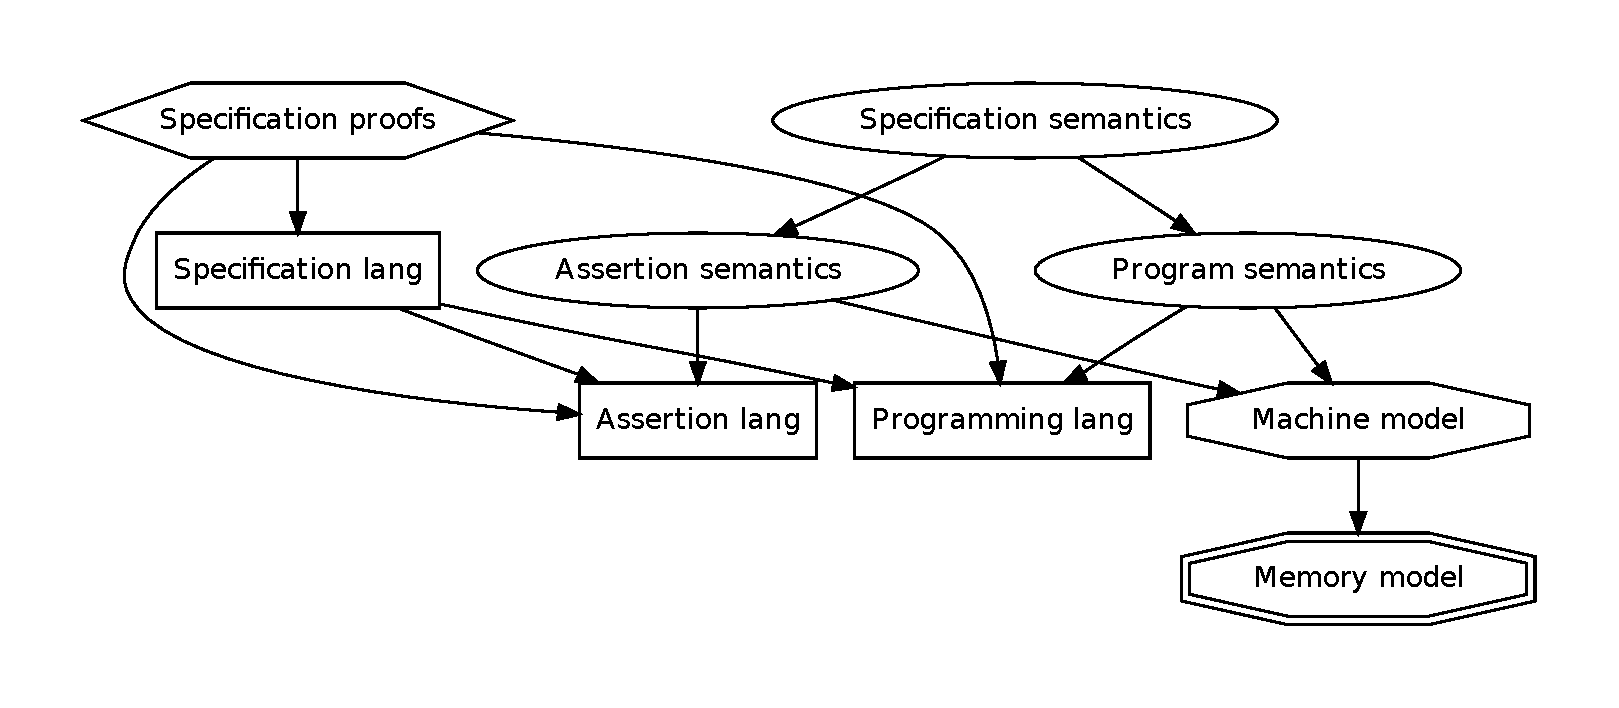
\includegraphics[scale=0.5]{dependency-graph/dg-reduced}
\caption{\label{fig:dependency-graph}Dependency graph for the project.}
%\end{center}
\end{figure}

The memory model is shown in a double-lined octagon, which reflects the assumption in this project that it is complete and correct, and is not further modified from its operational definition in \cite{DBLP:conf/tphol/OwensSS09}, which is summarized in Section~\ref{sec:memory-models}. 

The machine model---in particular, the notion of machine state---depends on, but is distinct from, the memory model. For example, the memory model dictates that each processor has a private set of named registers, whereas in the machine models that we shall define, a single share set of variable names is assumed. We will also take the liberty in the machine model to relax other restrictions on the notion of state from the memory model, such as the requirement that writes buffered by a single processor are totally ordered. 

The programming language is a structured C-like language with concurrent composition. It does not explicitly depend on any other components of the project. The programming language semantics relates the programming language to the machine model, and hence depends on them both. The uniprocessor machine model and sequential programming language are described in Section~\ref{sec:sequential-programs}; the multiprocessor machine model and concurrent programming language are described in Section~\ref{sec:programming-language}. 

The assertion language also does not explicitly depend on any other components of the project.\footnote{Implicitly, of course, it depends significantly on the memory and machine models.} The assertion language semantics associates the assertion language to sets of machine states (as defined by the machine model) with a particular structure. Assertions about uniprocessor machine states are described in Section~\ref{sec:uniprocessor-assertions}; assertions about multiprocessor machine states are described in Section~\ref{sec:assertions}. 

Ideally there would also be a proof theory of assertions and a corresponding soundness theorem. We have chosen not to focus on a proof theory of assertions in this project, but will indicate some semantic implications and equivalences that would be relevant to that end in Section~\ref{sec:sequential-algebra} for the uniprocessor case, and in Section~\ref{sec:algebra} in the multiprocessor case.

The specification language encompasses the programming and assertions languages, and its semantics is given in terms of the semantics of programs and assertions. The proof theory of specifications relies on the existence of a suitable proof theory of assertions for determining entailments. The soundness of the specification logic relies on the soundness of the proof theory of assertions as well as the semantics of programs and assertions. Specification of sequential programs are described in Section~\ref{sec:sequential-specifications}; specifications of concurrent programs are described in Section~\ref{sec:specifications}.

\subsection{Contributions and Status}

The significant contributions of this dissertation project are as follows:

\begin{enumerate}
  \item An x86-like operational semantics based on state transitions for a C-like programming language with pointers and pointer arithmetic, memory fences and concurrency constructs. The model is novel, and is expressive enough to describe both processor-parallel and interleaved thread executions. 

  \item An assertion language for describing, naturally and concisely, x86-like system configurations, and a formal semantics in terms of the aforementioned states. Both the language and the model are novel. 

  \item A program specification logic---i.e., a formal language of specifications and a proof system---for describing and deducing partial correctness of the aforementioned C-like programs in terms of the aforementioned assertions, as well as a formal semantics of specifications that relates the x86-like execution of C-like programs among states described by assertions. The specification logic additionally embodies an x86-specific principal of local reasoning, which allows proofs to be constructed by describing the interaction between the program and the small portion of system resources relevant to its behavior; and subsequently generalizing the proof to describe the interaction of the program with more complete system descriptions. This is the first known local reasoning principle for a weak memory model. 
\end{enumerate}

The languages, models and deduction system described above are completely and formally defined, having undergone hundreds of revisions. There are however two major components left unfinished: 
\begin{enumerate}
  \item There is no proof system for the assertion language. Omitting this component of the project was an early, intentional decision for two reasons. First, a proof system is necessary for practical application of the specification logic---and in particular automation of the specification logic---but is not critical for the study of the specification language. In practice, syntactic entailment is a practically important approximation of semantic entailment, but in principle simply having a well defined notion of semantic entailment is sufficient. Second, it is hypothesized that the traditional inference rules of first-order logic are sound for the assertion language defined here---as is the case for related theories of similar logics---and also that there is no complete set of rules---as this language encompasses, e.g., arithmetic. The task of finding a suitable proof system for the assertion can thus be seen as a purely practical issue.

  \item There is not a total soundness proof for the specification logic. Although the logic is hypothesized to be sound w.r.t.\ the model described later in the document, this is of course a serious drawback. Most of the relevant lemmas have been proved previously with various, preliminary versions of the model. There are no known problems with the model that are blocking a soundness proof beyond sheer size of the proof as derived from the complexity of the model. Indeed, the proofs are mostly straightforward inductions. Throughout the document, key intermediate properties that are expected to hold are noted along with proof sketches. 
\end{enumerate}

Finally, beyond these technical omissions, it must be admitted that this dissertation gives little indication of how proofs ought to proceed in the logic; only a handful of small examples will be given later on. This is because the logic has evolved with soundness to the x86 memory memory model foremost in mind, instead of as a logical system of interest independent of its potential models. Although the examples presented do indicate that the logic is capable of highly non-trivial program reasoning, the extent of its capability is not yet well understood, and remains as perhaps the most important aspect of future work. 

\chapter{Background}

This chapter describes background material necessary to understand the technical content of this dissertation, beginning with mathematical preliminaries and frequently used notation in Section~\ref{sec:preliminaries}, followed by an overviews of research on program logics in Section~\ref{sec:program-logics} and memory consistency models in Section~\ref{sec:memory-models}. 

\section{Mathematical Preliminaries}
\label{sec:preliminaries}

Terms are defined throughout this document with the following meta-notation: \[ \mathit{object} \eqdef \mathit{definition}.\] We additionally use the following meta-notation for defining predicates: \[ \mathit{predicate} \iffdef \mathit{definition}.\] For example, for a set $S$ and object $o \notin S$ we define \[S^o \eqdef S \uplus \set{o}\] as the extension of set $S$ by object $o$. Using this notation, a domain $S$ can be lifted to its \emph{optional domain} by writing $S^\bot$ as shorthand for $S \uplus \set{\bot}$, assuming $\bot \notin S$. 

\subsection{Relations}
\label{sec:relations}

For any set $A$, we write $\ident{A}$ for the identity relation on $A$. For a binary relation $R$ on $A$ and $n \in \setnaturals$, we write $\relexp{R}{n}$ for the $n$-fold iteration of $R$, defined by induction on $n$ as follows: \begin{align*} \relexp{R}{0} \eqdef &\ident{A} \\ 
\relexp{R}{n+1} \eqdef & \relexp{R}{n} \rcomp R.\end{align*} We write $\tcl{R}$ and $\rtcl{R}$ for the transitive and reflexive-transitive closures of $R$, respectively: \begin{align*}
    \tcl{R} \eqdef \bigcup_{n \in \setpositives} \relexp{R}{n} \andif
    \rtcl{R} \eqdef \bigcup_{n \in \setnaturals} \relexp{R}{n} 
\end{align*}

\subsection{Functions}
\label{sec:functions}

For a (possibly partial) function $f : A \pfun B$ and $a \in A$ and $b \in B$, we write $\funup{f}{\ptup{a}{b}}$ for the updated function: \[ \funup{f}{\ptup{a}{b}} \eqdef \fun{x} \begin{cases}
  b & \text{if $x = a$} \\
  f(x) & \text{otherwise.}
\end{cases}\] 

We write $f(a) = \bot$ if the partial function $f$ is not defined at point $a$, i.e. if $a \notin \dom{f}$, and $\defined{f(a)}$ otherwise. The everywhere-undefined function is indicated by $\nil$. The partial sum $f \uplus g$ of partial functions $f$ and $g$ is defined, when $\dom{f} \cap \dom{g} = \nil$, as follows: \[ f \uplus g \eqdef \fun{x}\begin{cases}
    f(x) & \text{if $x \in \dom{f}$} \\
    g(x) & \text{else if $x \in \dom{g}$} \\
    \bot & \text{otherwise.}
\end{cases}\]

 When convenient, we also write $f_a$ as shorthand for $f(a)$. $a \mapsto b$ is shorthand for the unique partial function $f$ such that $f(a) = b$ and is undefined otherwise. For $A' \subseteq A$, $\restrict{f}{A'}$ is the restriction of $f$ to domain $A'$. 

For (possibly partial) functions $f,g : A \pfun B$, we we write $f \override g$ for the result of \emph{overriding} $f$ with $g$: \[ f \override g \eqdef \fun{x} \begin{cases}
  g(x) & \text{if $x \in \dom{g}$} \\
  f(x) & \text{otherwise.}
\end{cases} \] An obvious property is that, if $g(a) = b$, for some $b \in B$, then also $(f \override g)(a) = b$. Some additional properties follow in Lemma~\ref{lem:override}. 

\begin{lemma}
    \label{lem:override}
    Let $f,g,h : A \pfun B$. 
    \begin{enumerate}
        \item $f \override \nil = \nil \override f = f$
        \item $f \override (g \override h) = (f \override g) \override h$. 
        \item $\dom{f \override g} = \dom{f} \cup \dom{g}$. 
        \item If $\dom{f} \cap \dom{g} = \nil$ then $f \override g = f \uplus g$, and hence $f \override g = g \override f$. 
    \end{enumerate}
\end{lemma}

\subsection{Lists}
\label{sec:lists}

The empty list is denoted by $\lnil$, the literal list by $\llit{o,\ldots, o'}$, list construction by $o \lcons l$, and list concatenation by $l \lapp l'$, for objects $o$ and lists $l$. We write $\listof{\mathcal{T}}$ to indicate lists of elements drawn from the set $\mathcal{T}$, and $\arnil$ for the function $(\fun{x} \lnil)$. 

For a list $l : \listof{(A \times B)}$, we write $\funof{l}$ for the corresponding partial lookup function: \[ \funof{l} \eqdef \fun{x} \begin{cases}
  b &\text{ if $l = l' \lapp \llit{(x,b)}$}\\
  \funof{l'}(x) &\text{ if $l = l' \lapp \llit{(y,b)}$ with $x \neq y$}\\
  \bot & \text{otherwise.}
\end{cases}\] For $A' \subseteq A$, $\restrict{l}{A'}$ is the sublist restriction of $l$ to domain $A'$.

For convenience, we lift these function definitions pointwise to sets of lists. For example, for a set $L$ of lists, $a \lcons L \eqdef \setof{a \lcons l}{l \in L}$. 

The set of \emph{interleavings} of lists $m,n$, written $m \merge n$, is defined by recursion on the structure of $m$ and $n$: \begin{align*}
  m \merge \lnil &\eqdef \set{m} \\
  \lnil \merge n &\eqdef \set{n} \\ 
  %a \lcons m' \merge b \lcons n' & \eqdef \bigcup_{l_b \in m' \merge (b\lcons n')} \, \bigcup_{l_a \in (a \lcons m') \merge n'} (a \lcons l_b) \merge (b \lcons l_a) \\ 
  a \lcons m' \merge b \lcons n' & \eqdef a \lcons (m' \merge (b\lcons n')) \cup b \lcons ((a \lcons m') \merge n').
\end{align*}

We now define a subset of the interleavings of lists of pairs from $A \times B$ that play an analogous role to function overriding. The result of overriding a list $m$ with another $n$, written $m \override n$, is defined as follows: \[ l \in m \override n \iffdef \funof{l} = \funof{m} \override \funof{n}.\] As with function overriding, list overriding has the property that, if $\funof{n}(a) = b$, for some $b \in B$, and $l \in m \override n$, then $\funof{l}(a) = b$. Because all elements of $m \override n$ have the same lookup function, we may safely extend the list lookup notation as follows: \[ \funof{m \override n} \eqdef \fun{x} \funof{l}(x),\] for arbitrary $l \in m \override n$. 

As for function overriding, list overriding has the basic property that, if $a \in \dom{\funof{n}}$, then $\funof{n}(a) = \funof{n \override m}(a)$. It also has the other following analogous properties, as noted by Lemma~\ref{lem:list-override}. 
\begin{lemma}
    \label{lem:list-override}
    Let $l,m,n : \listof{A \times B}$. 
    \begin{enumerate}
        \item $l \override \nil = \nil \override l = l$
        \item $l \override (m \override n) = (l \override m) \override n$. 
        \item $\dom{\funof{m \override n}} = \dom{\funof{m}} \cup \dom{\funof{n}}$. 
        \item If $\dom{\funof{m}} \cap \dom{\funof{n}} = \nil$ then $m \override n = m \merge n$, and hence $m \override n = n \override m$. 
        \item $(m \lapp n) \in (m \override n) \subseteq (m \merge n)$.
    \end{enumerate}
\end{lemma}


\subsection{Universes}
\label{sec:universes} 

The various universal sets are declared and in some cases defined in Figure~\ref{fig:universes}. Note that, in the case of memory locations (i.e., addresses into memory) and processor identifiers, 0 is excluded. Also note that we shall later use the single set of identifiers $\setidentifiers$ to represent both program variables and logical variables.

\begin{figure}[ht]
  \centering
  \begin{tabular}{rcl|l}
    \multicolumn{3}{c}{Set} & Description \\ \hline
    \multicolumn{3}{l|}{$\setidentifiers$} & Identifiers \\
    $\setvalues$ & $=$ &  $\setintegers$ & Values \\
    $\setlocations$ & $\subseteq$  &  $\setpositives$ & Memory locations \\
    $\setprocessors$ &$\subseteq$ &  $\setpositives$ & Processor identifiers
  \end{tabular}
  \caption{\label{fig:universes}Universal Sets}
\end{figure}


\section{Program Logics}
\label{sec:program-logics}

Given that the motivating problem is to reason about concurrent programs executing on a particular memory model, how might one approach the correctness of the program in Figure~\ref{fig:dekker} and others like it such as concurrent data structures? One solution---perhaps, for now, the best---is to reason directly about the program semantics in the following way:
\begin{enumerate}
\item formalize the semantics of the programming language using a general purpose logic (e.g., first-order logic, higher-order logic, type theory);

\item prove that the semantics agrees with the memory model;

\item characterize the intended program property using the general logic; 

\item prove using the general logic that the semantic object which represents the program at hand possesses this property.
\end{enumerate} 
This is a perfectly reasonable strategy and, by using a proof assistant for a selected general purpose logic (e.g., ACL2 \cite{DBLP:journals/tse/KaufmannM97}, Isabelle/HOL \cite{DBLP:books/sp/NipkowPW02}, or Coq \cite{CoqBook}), is within the realm of feasibility for some programs and some experts. But, due to the generality of the logic and complexity of the semantics of programs under study, one expects such proofs to be exceptionally complex. And although experts would certainly develop methodologies and abstractions to tame this complexity, the desire to reason at a higher and more intuitive level is manifest.

This is just the purpose of a \emph{program logic}, which allows high-level formal reasoning that codifies the programmer's intuition about the behavior and correctness of the program under study. Ideally, the program logic incorporates those methodologies and abstractions that have been most useful to expert users reasoning directly about semantic objects in more general logics.

The situation is analogous to the use of temporal logics for studying reactive systems. Though it is technically possible to reason about about such systems using a general-purpose logic, both human reasoning (e.g., Unity \cite{unity-book}) and automation (e.g., model checking \cite{model-checking}) were facilitated by specialized logics.

\subsection{Hoare Logic}
\label{sec:hoare-logic}

Hoare introduced the first program logic for an Algol-like language in his seminal 1969 paper \cite{DBLP:journals/cacm/Hoare69}. A program $c$ is specified with a pair of assertions $P$ and $Q$, written in first-order logic, that describe pre- and post-execution system states, respectively. Hoare described two related logics, which differ in the style of specification: in the \emph{total correctness} logic specifications are written $\left\langle P \right\rangle c \left\langle Q \right\rangle$ and require program termination as a necessary condition for satisfaction; in the \emph{partial correctness} logic specifications are written $\htriple{P}{c}{Q}$ and allow divergent executions of the program to satisfy \emph{any} specification. In the sequel, we focus on logics of partial correctness. 

The axioms and inference rules are either \emph{structural}, directed by the program syntax, or \emph{logical}, directed by the logical operations of the assertion language. The \textsc{choice} rule, for reasoning about nondeterministic choice command $\cchoice{c}{c'}$, is an example of a structural rule: \infrule[choice]{\htriple{P}{c}{Q} \andif \htriple{P}{c}{Q} }{\htriple{P}{\cchoice{c}{c'}}{Q}} According to this rule, in order to prove a specification $\htriple{P}{\cchoice{c}{c'}}{Q}$, it suffices to prove the same specification of each of the constituent commands: $\htriple{P}{c}{Q}$ and $\htriple{P}{c'}{Q}$. This is because the nondeterministic choice command may execute either $c$ or $c'$, but not both; and so if each constituent command satisfies the specification, then so must the composed command. 

The \textsc{disj} rule, for reasoning about specifications in which the primary connective of the precondition is a logical disjunction, is an example of a logical rule: \infrule[disj]{\htriple{P}{c}{Q} \andif \htriple{P'}{c}{Q}}{\htriple{P \disj P'}{c}{Q}} According to this rule, to prove a specification of an arbitrary comment in which the precondition is a disjunction, it suffice to prove a specifications in which the preconditions consist of each of the disjuncts. Intuitively, regardless of whether the command is executed in a state that satisfies $P$ or $P'$ it shall terminate in a state that satisfies $Q$, or diverge. 

The structural and logical rules of Hoare logic make proof construction partially mechanical. But determining whether a program meets its specifications remains generally undecidable due to the expressiveness of the assertion language. For example, the \emph{rule of consequence} allows for the relaxation of specifications by the arbitrary strengthening of preconditions and weakening of postconditions: \infrule[cons]{P' \Rightarrow P \,\,\,\,\,\, \left\lbrace P \right\rbrace c \left\lbrace Q\right\rbrace \,\,\,\,\,\, Q \Rightarrow Q' }{\left\lbrace P' \right\rbrace c \left\lbrace Q' \right\rbrace} For correct application of the rule, validity of the first-order logic implications must be proved. But first-order validity is, of course, undecidable in general, so while Hoare logic does ease some of the pain of proof construction, it is not a panacea.

%% Hoare logic has been thoroughly studied since its
%% introduction. Notably, it has been shown to be complete, in the sense
%% that true program specifications are provable if validity of
%% implications between assertions can be determined.

\subsection{Separation Logic}
\label{sec:separation-logic}

As successful as Hoare Logic has been, a significant drawback is its inability to soundly cope with pointer variables and dynamically allocated memory, thus severely complicating its application to low-level systems programs. To illustrate the problem, consider a simple program that updates the value at an address $x$ by writing to a dereferenced pointer: $\cstore{x}{2}$. To be clearly, this program does not update the value $x$, but instead the value in memory at the address whose value is $x.$. If we write $\mathit{heap}(x) = 2$ to mean that the value in memory address $x$ is equal to 2, then the following specification is clearly true: \[ \htriple{\mathit{heap}(x) = 1}{\cstore{x}{2}}{\mathit{heap}(x)=2}.\] We might then wish to prove a stronger specification, which describes the behavior of this program in a larger memory, with two allocated addresses $x$ and $y$: \[ \htriple{\mathit{heap}(x) = 1 \conj \mathit{heap}(y) = 1}{\cstore{x}{2}}{\mathit{heap}(x)=2 \conj \mathit{heap}(y) = 1}. \] This is easily derivable in Hoare logic using the \emph{rule of constancy}, which allows an arbitrary\footnote{Actually, there is a simple syntactic restriction on $F$: namely, that $\fv{F} \cap \mod{c} = \nil$; i.e., that the free variables of the frame are not modified by the command. This holds in the example because no variables are modified by dereferencing assignment.} assertion $F$---called a \emph{frame}---to be conjoined uniformly onto the pre- and post-conditions of a derived specification: \infrule[const]{\htriple{P}{c}{Q}}{\htriple{P \conj F}{c}{Q \conj F}.} The problem, of course, is that this strengthened specification is not true. In case the pointer variables $x$ and $y$ are \emph{aliased}---i.e., if $x = y$---after the pointer update it shall certainly not be the case that $\mathit{heap}(y) = y$, for the update to the memory at $x$ also implicitly updated the memory at $y$. 

In the presence of pointer variables, the rule of constancy---which is crucial to the scalability of Hoare logic---is only sound in case the memory locations referred to by the frame are disjoint or separate from those in the \emph{footprint} of the command; i.e., the part of the system state referenced by the program during its execution. To maintain soundness, therefore, proofs in Hoare logic about such programs require a variety of ad hoc extensions and onerous side conditions. (See, e.g., Richard Bornat's 2000 paper \cite{DBLP:conf/mpc/Bornat00}, which incorporates many sophisticated ideas into Hoare logic.) But after more than forty years of research, a major breakthrough finally came with the invention of \emph{separation logic} \cite{DBLP:conf/lics/Reynolds02}, generally credited to John Reynolds and Peter O'Hearn. A Hoare-style program logic (insofar as the axioms and inference rules are similar), the crucial difference between it and Hoare logic is the assertion language. Instead of the classical first-order logic assertions used by Hoare logic specifications, separation logic makes use of a different logic---a theory of the logic of \emph{bunched implications} pioneered by O'Hearn, Pym and others \cite{DBLP:journals/bsl/OHearnP99,DBLP:journals/tcs/PymOY04}---for describing system states with a notion of a \emph{heap}---a finite partial function, into which pointers point, that represents part of memory---and disjointness of said states. The salient formulas that capture these notions are the \emph{points-to assertion}, $\ell \mapsto v$, and the \emph{separating conjunction}, $P \fsep Q$. Models of the first formula are heaps with exactly one address allocated, given by $\ell$, and with value $v$ stored at that address: i.e., $h \sentails \ell \fpointsto v$ iff $h = \set{(\ell,v)}$. Models of the second formula are heaps that can be partitioned by address into two subheaps, one of which models the formula $P$ and the other $Q$: i.e., $h \sentails P \fsep Q$ iff $h = h_P \uplus h_Q$ such that $h_P \sentails P$ and $h_Q \sentails Q$. 

Besides soundness w.r.t.~a sequential C-like language with pointers and dynamic memory management, separation logic is important because it embodies the principle of \emph{local reasoning}. Unlike with Hoare logic, reasoning may be restricted to a program component's footprint, from which one may generalize to complete system states. O'Hearn, Reynolds and Yang informally describe local reasoning in the context of sequential pointer programs as follows \cite{DBLP:conf/csl/OHearnRY01}: \begin{quotation}\noindent To understand how a program works, it should be possible for reasoning and specification to be confined to the [memory addresses] that the program actually accesses. The value of any other [addresses] will automatically remain unchanged.\end{quotation}

Separation logic embodies the principle of local reasoning with its \emph{small axioms} and its \emph{frame rule}. The small axioms describe the programming language's primitive commands, specifying only their respective footprints. For example, the small axiom\footnote{Actually, an axiom schema parametrized by the expressions $e$ and $e'$.} for the pointer assignment command (i.e., store command) requires with its precondition only that the relevant location be allocated with some value,\footnote{$e \mapsto -$ is shorthand for $\exists v\,.\,e \mapsto v$.} and the resulting postcondition describes only the result of updating this location: \infax[store]{\left\lbrace e \mapsto -\right\rbrace \,\left[e\right] := e' \,\left\lbrace e \mapsto e'\right\rbrace} The local specification can then be generalized to a global specification using the \emph{frame rule}:\footnote{As in the rule of constancy, the frame rule also requires that $\fv{F} \cap \mod{c} = \nil$.}  \infrule[frame]{\htriple{P}{c}{Q}}{\htriple{P \fsep F}{c}{Q \fsep F}} The frame rule of separation logic replaces the rule of constancy of Hoare logic. It can be used to soundly derive the desired specification for the aforementioned program as follows: \[ \infer[\textsc{frame}]{\htriple{x \fpointsto 1 \fsep y \fpointsto 1}{\cstore{x}{2}}{x \fpointsto 2 \fsep y \fpointsto 1}}{\infer[\textsc{cons}]{\htriple{x \fpointsto 1}{\cstore{x}{2}}{x \fpointsto 2}}{\infer[\textsc{store}]{\htriple{x \fpointsto - }{\cstore{x}{2}}{x \fpointsto 2}}{}}}\]

Besides having been used to give human-readable proofs to a variety of algorithms that manipulate complex pointer-based data structures (e.g., the Schorr-Waite graph-marking algorithm \cite{Yang-thesis}), useful fragments of separation logic have been automated as part of program verifiers and static analyses, which have been successfully applied to programs with tens of thousands of lines of source code~\cite{DBLP:conf/fmco/BerdineCO05,DBLP:conf/cav/YangLBCCDO08,DBLP:conf/cav/BerdineCI11}.

\subsection{Concurrent Program Logics}

Research into logics for concurrent programs has progressed independently from research into logics for increasingly expressive sequential programs. Major efforts are summarized below. 

\paragraph{The Owicki-Gries Logic} Early attempts at handling concurrency within a program logic culminated in an extension of Hoare logic by Owicki and Gries \cite{DBLP:journals/cacm/OwickiG76}, which adds a rule for parallel composition of two program components with the cumbersome side condition that every assertion in one component's specification be invariant under the operation of each atomic command executed by the other component. While elegant in its simplicity, the side condition restricts the logic's usefulness. First, every application of the parallel composition rule requires a number of invariant proofs quadratic in the size of the components, making scalability difficult. Second, the side condition creates dependencies on the \emph{proofs} of the component specifications, not just on the specifications themselves. This effectively rules out independent proof construction for the individual components and yields a highly non-compositional logic.

\paragraph{Rely/Guarantee} Some relief from these problems was provided by Jones in his rely/guarantee logic \cite{JonesRelyGuar}, in which Hoare-style specifications are augmented with two additional assertions: the \emph{rely} condition, which bounds the interference from the environment that a component can tolerate while still meeting its pre- and post-specifications; and the \emph{guarantee} condition, which bounds the interference the program itself may inflict upon the environment. Application of the rely/guarantee parallel composition rule requires proofs that each process' rely condition subsumes the others' guarantee conditions.

While a considerable improvement over the Owicki-Gries logic---subsumption proofs linear in the number of components versus quadratic in their size, and dependence only among components'specifications instead of their proofs---rely/guarantee still has shortcomings. The logic cannot be considered truly compositional because each component may be specified with a variety of interference conditions, and it is not clear which are appropriate until attempting the parallel composition. Furthermore, it can be laborious to specify sufficiently strong guarantee conditions. For example, the guarantee condition for a component with three variables ($x,y,z$) that updates only one ($x := x+1$) must describe not just the relevant variable change ($x' = x + 1$), but also that all others remain the same ($\ldots \wedge y' = y \wedge z' = z$)---the latter condition being difficult because it suggests a sort of quantification over variable names not possible in first-order logic, instead requiring an explicit numeration of state variables.

\paragraph{RG-Sep} A partial solution to this problem of specification has recently appeared via separation logic. A new concurrent program logic from Vafeiadis and Parkinson, dubbed RG-Sep \cite{DBLP:conf/concur/VafeiadisP07} (``a marriage of rely/guarantee and separation logic''), mates a generalization of separation logic's assertion language and frame rules with the rely/guarantee logic. Besides inheriting the local reasoning features of separation logic, RG-Sep eases the pain of specifying environmental interference by semantically partitioning the system state into private and shared parts. A new class of boxed assertions $\boxed{P}$ is used to describe shared state, and the logical operations are adjusted so that, e.g., a separated conjunction of boxed assertions $\boxed{P} * \boxed{Q}$ allows their footprints to overlap.\footnote{An interesting consequence is that $\boxed{P} * \boxed{Q}$ is logically equivalent to $\boxed{P \wedge Q}$.} The proof rules are then modified so that, e.g., parallel composition requires only that each component be tolerant of environmental interference to shared state, not private state. This could be used in the previous example to obviate the explicit enumeration needed to describe invariance of the irrelevant state variables.

RG-Sep embodies some of the most advanced ideas about high-level reasoning techniques for fine-grained concurrent shared-memory programs, including local reasoning. Vafeiadis' 2008 dissertation \cite{VafeiadisDissertation} includes correctness proofs for a variety of complex, racy concurrent data structures using the logic. RG-Sep is by no means simple, but does yield relatively concise, readable proofs about difficult algorithms. Indeed, the only significant criticism I provide here is that, as with all the other concurrent logics discussed, RG-Sep is not sound w.r.t.~weak memory models for racy programs.

\paragraph{Concurrent Separation Logic} A simplified variant of the original Owicki-Gries logic does away with the complicated interference side condition, instead restricting its scope to well locked\footnote{The exact definition of ``well locked'' is technical and rather complicated, but purely syntactic, and hence preferable to the logical interference side conditions imposed by the full Owicki-Gries logic.} and race-free programs. For this smaller (but still large and useful) class of programs, it is possible to use the Owicki-Gries logic to perform \emph{invariant-based} reasoning, in which threads' interaction with shared state may rely only on a specified invariant, and must always preserve that same invariant.

As with Jones' original rely/guarantee logic, this simplified Owicki-Gries logic suffers from the difficulty of constantly having to specify, at each step of the proof, not just what has changed in the progrma state, but also what has not changed. Once again, the solution is to incorporate the concurrent reasoning of the simplified Owicki-Gries logic in a separation logic-style logic. This logic, called Concurrent Separation Logic (CSL), originally developed by Peter O'Hearn and Stephen Brookes \cite{DBLP:journals/tcs/OHearn07,DBLP:journals/tcs/Brookes07}, does just that. Hoare-style specifications are elaborated with an invariant $I$: \[ \spec{I}{P}{c}{Q},\] which indicates informally that, from a state which can be partitioned into a shared part, which satisfies $I$, and a private part, which satisfies $P$, that 1) the program $c$ does not ever encounter a memory error; 2) that throughout execution the some portion of the state always satisfies $I$; and 3) if the program terminates, then it does in a state which can be partitioned finally into a shared part that satisfies $I$ and a private part that satisfies $Q$. The \textsc{par} rule for reasoning about the parallel composition of program components $c$ and $c'$ is, by comparison with the other approaches, extremely simple: \infrule[par]{\spec{I}{P}{c}{Q} \andif \spec{I}{P'}{c'}{Q'}}{\spec{I}{P \fsep P'}{c \oppar c'}{Q \fsep Q'}} This rule asserts that if $c$ and $c'$ can be proved to maintain the same invariant along with their own private specifications, then the the parallel combination $c \oppar c'$ must also maintains that invariant and, assuming the private portions of state accessed by the two components are disjoint, maintains their private specifications as well. 

\section{Memory Consistency Models}
\label{sec:memory-models}

A \emph{memory consistency model} (or just \emph{memory model}) is a specification of a concrete implementation of a shared memory system. Memory consistency models bound the possible results of reading an address in shared memory according to the history of writes and reads that have already taken place or are in progress. For the sake of reasoning about the behavior of concurrent software programs interacting with a shared memory, memory concistency models are a crucial abstraction: not only are concrete implementations of shared memory in modern computer systems are incredibly complex, but their details may additionally be considered proprietary and secret.\footnote{As a consequence of this complexity and secrecy, it can be challenge to determine whether or not a memory implementation is soundly described by a particular memory consistency model. This interesting problem is beyond the scope of this project.}  

Many memory consistency models have been defined and studied \cite{SteinkeNutt,higham98weak,DBLP:journals/computer/AdveG96}. Below, we discuss (informally) two of particular interest: sequential consistency, the most commonly used abstraction of memory for well-behaved programs; and the x86-TSO memory model, which describes the interaction between memory and arbitrary software programs on x86-like multiprocessor computers. 

\subsection{Sequential Consistency} 
\label{sec:sc}

Sequential consistency was originally defined by Leslie Lamport in 1979 \cite{DBLP:journals/tc/Lamport79}. For a sequentially consistent program, he wrote: \begin{quotation}\noindent the result of any execution is the same as if the operations of all the processors were executed in some sequential order, and the operations of each individual processor appear in this sequence in the order specified by its program. \end{quotation} 

As an example, consider again the program in Figure~\ref{fig:dekker}, in which thread 0 writes to $f_0$ and then reads from $f_1$; and thread 1 writes to $f_1$ and reads from $f_0$. If we write $(p,o,\ell,v)$ to indicate that thread $p$ performs operation $o$ (where $o \in \set{r,w}$ is either a read or a write) on location $\ell$ with value $v$ (indicate the value written or value read), then: \[ (0,w,f_0,1), (1,w,f_1,1), (1,r,f_0,1), (0,r,f_1,1)\] is a sequentially consistent execution, because the operations of each thread occurs, within the execution, in the same order as the operations appear in their respective programs (with the writes preceding the reads), and the results of the loads clearly are consistent with the total order of operations given. 

On the other hand, the following two executions are not sequentially consistent: \begin{align*}
  (0,r,f_1,0), (1,w,f_1,1), (1,r,f_0,0), (0,w,f_0,1) \\ 
  (0,w,f_0,1), (0,r,f_1,0), (1,w,f_1,1), (1,r,f_0,0), 
\end{align*} In the first execution, it is not the case that the operations of thread 0 take place in the order specified by the program: the read precedes the write. In the second execution, the order of operations is consistent with the order specified by the program, but the result is not the same as if the operations were executed in that order: the final read of $f_0$ by thread 1 should not result in value 0, because it directly succeeds the write to $f_1$. 

Operationally, this constraint on the possible execution traces of a program can be realized by modeling memory as a simple location-value map, in which reads and writes to memory happen occur atomically. That is, memory is represented by a (possibly partial) function $\setlocations \pfun \setvalues$; and the semantics of the program is defined such that no more than one thread may read or update the memory at once. This, of course, is the most widespread model of memory used in the semantics of imperative, shared-memory programs, and consequently the vast majority of program reasoning and verification techniques tacitly assume that programs are sequentially consistent; i.e., that all its executions can be described by its interactions with this simple model of memory. 

\subsection{The x86-TSO Memory Model}
\label{sec:x86-TSO}

After a great deal of investigation, experimentation and discussion with manufacturers, Owens, Sarkar and Sewell published a specification \cite{DBLP:conf/tphol/OwensSS09} of the x86 memory model. This model has become widely accepted as accurate \footnote{An earlier paper \cite{DBLP:conf/popl/SarkarSNORBMA09}, suggested that the x86 memory model more closely resembled \emph{causal consistency}---a model in which there is a single agreed-upon order not just for the store events, but for all causally related memory events---but this was later contradicted by counterexamples that lead to the current proposed TSO model.} and forms the basis for a great deal of related research---e.g., the Comp-Cert project-in-progress \cite{Leroy-Compcert-CACM}, which attempts to construct a realistic (i.e., which performs realistic optimizations) and formally verified compiler for C and C++. 

The model identified by Owens et al.~is essentially a \emph{total-store order} (TSO) model which, as the name implies, indicates that there is a single total order, agreed upon by all processors, that organizes store events. Their x86-TSO model is described as a collection of legal traces of memory events, defined both axiomatically and operationally. The latter, informally, is described in terms of \emph{write buffers}: per-processor FIFO queues of ``writes'' (i.e., location-value pairs). The informal semantics of store events entails buffering a new write in the processor's write buffer; the semantics of load events entails returning the value of the most recent buffered write to the intended location in the processor's write buffer or, if no such buffered write exists, in the shared memory. 
 
Formally, the operational model is given with a labeled transition relation between machine states. These states are four-tuples $(R,m,B,l)$ in which: \begin{itemize}
	\item $R : \setprocessors \tfun \setidentifiers \pfun \setvalues$ represents a register file for each processor;
	\item $m : \setlocations \pfun \setvalues$ represents a shared memory; 
	\item $B : \setprocessors \tfun \listof{(\setlocations \times \setvalues)}$ represents a write buffer for each processor; 
	\item $l : \setprocessors^\bot$ represents a global lock. 
\end{itemize}

Transitions (labeled by memory events) between states indicate the possibility and effect of those memory events. For example, in any state $(R,m,B,l)$, processor $p$ may write a value $v$ into its register $i$; i.e., it may update the state such that $R_p(i) = v$. Similarly, if $R_p(i) = v$ then $p$ may read value $v$ from its register $i$. A summary of the other events processor $p$ may perform is as follows: \begin{itemize}
	\item it may load from its write buffer the most recent value of a location---or, if a write to that location is not found in its write buffer, from memory---if the lock is either available ($i.e.$, the lock value is $\bot$) or is held by $p$, but not if some other processor $q \neq p$ holds the lock;
	\item it may store a value to a memory location by adding a new write to the head of its write buffer regardless of the status of the lock; 
	\item it may flush (or, synonymously in this document, commit) the least recent write in its buffer to memory if it holds the lock or the lock is available;  
	\item it may fence if its buffer is empty;
	\item it may acquire the lock (i.e., change the lock value in the current state to $p$) if the lock is available; 
	\item it may release the lock (i.e., change the lock value in the current state to $\bot$) if it holds the lock.
\end{itemize}

The x86-TSO memory model includes all the sequentially consistent executions, as well as others. For example, the sequentially consistent execution from the previous section: \[ (0,w,f_0,1), (1,w,f_1,1), (1,r,f_0,1), (0,r,f_1,1), \] is shown valid (informally) under the x86-TSO model as follows. Assume that no processors hold the lock. The first thread may perform its store operation by enqueuing a write $(f_0,1)$ in its buffer, and then immediately flushing that write to memory; and then similarly for the second thread, which enqueues a write $(f_1,1)$ and then immediately flushes it to memory. If then the second thread then reads location $f_0$ it finds value 1 (because it has no other writes to $f_0$ in its buffer); and similarly if the first thread then reads location $f_1$ it finds value 1 for the same reason. 

Next, consider again the two non-sequentially consistent executions of Figure~\ref{fig:dekker} from the previous section: \begin{align*}
  (0,r,f_1,0), (1,w,f_1,1), (1,r,f_0,0), (0,w,f_0,1) \\ 
  (0,w,f_0,1), (0,r,f_1,0), (1,w,f_1,1), (1,r,f_0,0), 
\end{align*} The first non-sequentially consistent execution is invalid w.r.t.\ the x86-TSO model as well, because the operations of a single thread still take place in the order specified by the program. The second non-sequentially consistent execution, however, is valid under the x86-TSO model: the first process enqueues a write $(f_0,1)$ in its buffer, and then reads $0$ from location $f_1$ in memory (because its buffer contains no writes to $f_0$); then the second process enqueues a write $(f_1,1)$ in its buffer, and then reads $0$ from location $f_0$ in memory (because its buffer has no writes to $f_1$, only the other buffer). 

When combined with the earlier claim that the x86-TSO memory model also includes all sequentially consistent executions, this example shows that x86-TSO memory model is strictly weaker than sequential consistency. Consequently, x86-TSO is considered to be a \emph{weak memory model}.

Note that, despite the completely informal examples above, this specification of the x86-TSO memory model only \emph{bounds} the sort of memory events that can occur in program executions; it does not give meaning to the programs of any particular particular language, like x86 assembly or C programs. It can, however, be used to give semantics to programs in those languages. Owens et al.\ use their semantics to assign semantics to a significant subset of the x86 assembly language, for example. The semantics of the simple C-like programming language used in this dissertation project is also guided by the x86-TSO memory model. And although it should be possible to prove that it respects the bounds of the model, this is not the focus of the project. But even without such a correspondence proof, it is clear that the semantics of the programming language described later is manifestly weak. 

\subsection{Data-Race-Freedom Guarantees} 
\label{sec:drf}

Although the memory models of most modern computer architectures---including, as we have seen, x86-like computer architectures---are relatively weak, allowing additional executions compared to a sequentially consistent memory model, the tacit assumption that programs are sequentially consistent made by most verification techniques is actually, in many cases, perfectly reasonable. This is because modern computer architectures, including x86, guarantee sequentially consistent execution for a large class of programs: namely, the data-race free programs. Because of these so-called data-race-freedom (DRF) guarantees, verification techniques which assume sequential consistency are perfectly sound in case the program under consideration is race-free. And because races are generally considered to be errors, a reasonable verification workflow is to first check that a program is race-free before proceeding with the verification of more elaborate properties; or, alternatively, to leverage techniques which succeed only for race-free programs. But not all correct programs are race-free; for these programs, verification techniques may need to account for the full complexities of the underlying memory model. 

\chapter{A Sequential Program Logic}
\label{ch:uniprocessor}

In this chapter we describe a program logic for a sequential, single-processor, weak-memory programming model. The semantics of programs and assertions will be given in terms of system states with a single write buffer, and the logic is tailored to reason about the behavior of sequential programs w.r.t.\ these states. The logic developed in this chapter is not especially useful; the behavior of sequential program execution on this model is essentially the same as on the typical, strong-memory model (in which memory is modeled as a single array of addresses), and existing logics for reasoning about this behavior are certainly simpler than the one developed here. But the sequential program logic is a pedagogical stepping stone toward the concurrent program logic, for which the behavior of programs may well be significantly different from that of a strong-memory model. The development of the sequential logic is vastly simpler than the weak-memory, multi-processor logic, and many of the more difficult issues in that task can be introduced and explained more easily in a single-processor setting. 

A detailed description and soundness proof of a single-processor, weak-memory program logic was given previously \cite{wmsldetails}. 

\section{An Example Proof}

Consider the following simple sequential program $c$, which loads the value at an address $x$ into variable $t$, writes the value $t+1$ into address $y$, and then flushes that write back to memory with a fence instruction: \[ c \eqdef \cload{t}{x} \opseq \cstore{y}{t+1} \opseq \cfence.\] This sequential program will fail with a memory error unless the value of $x$, from which the program loads, is a properly allocated memory address, as well as the value $y$, to which the program writes. Any provable specification of this program must require this of $x$ and $y$ initially. If the value of $x$ and $y$ are indeed allocated addresses, and the value in memory at address $x$ is initially some value $z$, then upon termination the write buffer will be empty and the value in memory at location $y$ will be $z+1$. 

In the program logic we develop throughout this chapter, we express this informal specification of $c$ with the following formal specification: \begin{align}\label{eq:seq-ex-spec} \triple{(x \fpointsto z) \fsep (y \fpointsto -)}{c}{(x \fpointsto z) \fsep (y \fpointsto (z + 1))}.\end{align}
We write $e \fpointsto f$ to mean that the value in memory at the address given by the integer-valued expression $e$ is equal to the value given by expression $f$, or $e \fpointsto -$ if the value in memory at $e$ is irrelevant. We also write the \emph{separating conjunction} $e \fpointsto f \fsep e' \fpointsto f'$ to mean that $e$ and $e'$ are distinct, allocated memory addresses, with values in memory given by $f$ and $f'$ respectively. Hence, the precondition on the left asserts that $x$ and $y$ are allocated memory locations, the former with value $z$, and the postcondition on the right asserts that, upon executing the command $c$, the value at $x$ remains $z$ and the value at $y$ has been set to $z+1$. 

Note that the specification in Equation~\ref{eq:seq-ex-spec} above would not be true if the traditional \emph{additive conjunction} $\conj$ were used instead of the separating conjunction. That is, the following specification: \[ \triple{(x \fpointsto z) \conj (y \fpointsto -)}{c}{(x \fpointsto z) \conj (y \fpointsto (z + 1))}.\] is not true because it allows for $x$ and $y$ to be \emph{aliased}---i.e., to denote the same memory address. For in that case the store to $y$ would change the value in memory at $y$ as well as at $x$, leaving $x \fpointsto (z+1)$ instead of $x \fpointsto z$ as specified. Also note that the specification in Equation~\ref{eq:seq-ex-spec} would not be true without the trailing $\cfence$ command because the buffered write will not necessarily have committed to memory at the moment the commands have completed their execution. 

A \emph{proof sketch} of the program specification in Equation~\ref{eq:seq-ex-spec} is as follows, the details of which will be explained shortly:
\Sketch{
  
  \aconn{$(x \fpointsto z) \fsep (y \fpointsto -)$}

  \acomm{$\cload{t}{x}$}

  \aconn{$(x \fpointsto z) \fsep ((y \fpointsto -) \conj t = z)$}

  \acomm{$\cstore{y}{t+1}$}

  \aconn{$(x \fpointsto z) \fsep ((y \fpointsto -) \fseq (y \fwriteu (z+1))) $}

  \acomm{$\cfence$}

  \aconnl{$(x \fpointsto z) \fsep (y \fpointsto (z+1))$}

}
As the name indicates, a proof sketch provides a skeleton of a complete proof of a program specification. For a program $c_1 \opseq c_2$, a proof sketch may take the form: 
\Sketch{

  \aconn{$P$}

  \acomm{$c_1$}

  \aconn{$R$}

  \acomm{$c_2$}

  \aconnl{$Q$}

} which indicates that a complete proof will include proofs of the sub-specifications $\triple{P}{c_1}{R}$ and $\triple{R}{c_2}{Q}$ that will be combined, in a final step, using a rule of inference (\textsc{seq}) for composing specifications of sequentially combined commands: 
\[ \infer[{\textsc{seq}}]{\triple{P}{c_1 \opseq c_2}{Q}}{\infer{\triple{P}{c_1}{R}}{\vdots} & \infer{\triple{R}{c_2}{Q}}{\vdots}}\] where the vertical dots represent the remaining proofs to be supplied. 

Returning to the proof sketch of the program specification in Equation~\ref{eq:seq-ex-spec}, we see that to complete the proof we must derive three sub-specifications, one for each primitive command: \begin{enumerate}
  \item $\triple{(x \fpointsto z) \fsep (y \fpointsto -)}{\cload{t}{x}}{(x \fpointsto z) \fsep ((y \fpointsto -) \conj t = z)}$
  \item $\triple{(x \fpointsto z) \fsep ((y \fpointsto -) \conj t = z)}{\cstore{y}{t+1}}{(x \fpointsto z) \fsep ((y \fpointsto -) \fseq (y \fwriteu (z+1)))}$
  \item $\triple{(x \fpointsto z) \fsep ((y \fpointsto -) \fseq (y \fwriteu (z+1)))}{\cfence}{(x \fpointsto z) \fsep (y \fpointsto (z+1))}$
\end{enumerate}
The first specification asserts that the result of loading the value $z$ in memory at address $x$ into variable $t$ results in a state that is otherwise unchanged except that $t = z$. The second specification asserts that the result of storing the value $t+1$ to the address $y$ results in the addition of a new buffered write to the state, which may later be committed to memory, overwriting the current, unspecified value. The third specification asserts that the result of explicitly flushing this write to memory overwrites the existing value in memory at $y$ with the value $z+1$. 

We shall now derive these three specifications. For the first specification, we start by using an instance of the \textsc{load} axiom scheme to show that the result of evaluating the load command $\cload{t}{x}$ from precondition $x \fpointsto z$ yields the postcondition $x \fpointsto z \conj t = z$.
\[ 
  \infer[\textsc{load}]{\triple{x \fpointsto z}{\cload{t}{x}}{x \fpointsto z \conj t = z}}{}
\] We then use the \emph{spatial frame rule} \textsc{frame-sp} to extend the pre- and post-condition with a description of the value of an additional, distinct memory address $y$: \[ 
  \infer[\textsc{frame-sp}]{\triple{(y \fpointsto -) \fsep (x \fpointsto z)}{\cload{t}{x}}{(y \fpointsto -) \fsep (x \fpointsto z \conj t = z)}}{
    \infer[\textsc{load}]{\triple{x \fpointsto z}{\cload{t}{x}}{x \fpointsto z \conj t = z}}{}
  }
\] Finally, we observe that the derived pre and postconditions are not syntactically equal to those of the desired specification, but are logically equivalent: \begin{align*}
(y \fpointsto -) \fsep (x \fpointsto z) \sequiv & (x \fpointsto z) \fsep (y \fpointsto -) \\ 
(y \fpointsto -) \fsep (x \fpointsto z \conj t = z) \sequiv & (x \fpointsto z) \fsep ((y \fpointsto -) \conj t = z)
\end{align*} More generally, the derived precondition is logically implied by the desired precondition, and the derived postcondition logically implies the desired postcondition. Hence, we may strengthen the precondition and weaken the postcondition accordingly with the rule of consequence \textsc{cons}: \[ 
  \infer[\textsc{cons}]{\triple{(x \fpointsto z) \fsep (y \fpointsto -)}{\cload{t}{x}}{(x \fpointsto z) \fsep ((y \fpointsto -) \conj t = z)}}{
    \infer[\textsc{frame-sp}]{\triple{(y \fpointsto -) \fsep (x \fpointsto z)}{\cload{t}{x}}{(y \fpointsto -) \fsep (x \fpointsto z \conj t = z)}}{
      \infer[\textsc{load}]{\triple{x \fpointsto z}{\cload{t}{x}}{x \fpointsto z \conj t = z}}{}
    }
  }
\] This completes the derivation of the first specification. 

For the second specification, we begin with an instance of the axiom scheme for the store command in which the precondition describes just the value of $y$ in memory: \[ \infer[\textsc{store}]{\triple{y \fpointsto -}{\cstore{y}{t+1}}{(y \fpointsto -) \fseq (y \fwriteu (t+1))}}{}\] The postcondition describes, with the \emph{leads-to} assertion $y \fwriteu  t+1$, the addition of a new, buffered write to address $y$ with value $t+1$. The \emph{temporal separating conjunction} $(y \fpointsto -) \fseq (y \fwriteu t+1)$ indicates that the writes described on the left side precede those on the right side. 

Next, we again apply the spatial frame rule \textsc{frame-sp} to extend the specification with a description of the value of memory at $x$ and the value of variable $t$: 
\[ \infer[\textsc{frame-sp}]{\triple{(x \fpointsto z \conj t = z) \fsep (y \fpointsto -)}{\cstore{y}{t+1}}{(x \fpointsto z \conj t = z) \fsep ((y \fpointsto -) \fseq (y \fwriteu (t+1)))}}{
  \infer[\textsc{store}]{\triple{y \fpointsto -}{\cstore{y}{t+1}}{(y \fpointsto -) \fseq (y \fwriteu (t+1))}}{}
  } \]

The derived precondition is logically equivalent to the desired precondition, and the derived postcondition logically implies the desired postcondition \begin{align*}
(x \fpointsto z \conj t = z) \fsep (y \fpointsto -) \sequiv & (x \fpointsto z) \fsep ((y \fpointsto -) \conj t = z))\\ 
(x \fpointsto z \conj t = z) \fsep ((y \fpointsto -) \fseq (y \fwriteu (t+1))) \sentails & (x \fpointsto z) \fsep ((y \fpointsto -) \fseq (y \fwriteu (z+1)))
\end{align*} Hence, we finish the derivation of the second specification with an application of the rule of consequence \textsc{cons}: 
\[ \infer[\textsc{cons}]{\triple{(x \fpointsto z) \fsep ((y \fpointsto -) \conj t = z)}{\cstore{y}{t+1}}{(x \fpointsto z) \fsep ((y \fpointsto -) \fseq (y \fwriteu (z+1)))}}{\infer[\textsc{frame-sp}]{\triple{(x \fpointsto z \conj t = z) \fsep (y \fpointsto -)}{\cstore{y}{t+1}}{(x \fpointsto z \conj t = z) \fsep ((y \fpointsto -) \fseq (y \fwriteu (t+1)))}}{
  \infer[\textsc{store}]{\triple{y \fpointsto -}{\cstore{y}{t+1}}{(y \fpointsto -) \fseq (y \fwriteu (t+1))}}{}
  }}
 \]

For the third and final specification, we begin with the axiom for the $\cfence$ command: \[ \infer[\textsc{fence}]{\triple{\femp}{\cfence}{\fbaru}}{}\] This small axiom allows for the introduction, from an empty system description, of the $\fbaru$ assertion. Intuitively, this assertion describes the effect of a barrier on the system state, in the sense that any writes that precede $\fbaru$ must necessarily be committed to memory. For example, we have the following logical equivalence: \[ y \fpointsto t+1 \sequiv (y \fwriteu t+1) \fseq \fbaru \] This means that the description of $y$ having value $t+1$ in memory is equivalent to the description of a buffered write to address $y$ with value $t+1$ followed by a flush of that write to memory.\footnote{In fact, the points-to assertion shall later on in the description of the sequential logic be made definitionally equal to the temporal conjunction of the analogous leads-to assertion and $\fbaru$. This equivalence will not necessarily hold in the concurrent logic, however.} We wish to describe the effect of $\fbaru$ on the postcondition from the previous specification, so we extend the specification accordingly with the \emph{temporal frame rule} \textsc{frame-tm}: 
\[ \infer[\textsc{frame-tm}]{\triple{((x \fpointsto z) \fsep ((y \fpointsto -) \fseq (y \fwriteu (z+1)))) \fseq \femp}{\cfence}{((x \fpointsto z) \fsep ((y \fpointsto -) \fseq (y \fwriteu (z+1)))) \fseq \fbaru}}{
\infer[\textsc{fence}]{\triple{\femp}{\cfence}{\fbaru}}{}}
\] The empty assertion is a unit w.r.t.\ both the spatial and temporal separating conjunctions, so the precondition assertion is equivalent to one without the final temporal conjunct $\femp$. And the postcondition is equivalent to one in which the buffered write has been flushed to memory, replacing the previous value in memory: \[ (x \fpointsto z) \fsep ((y \fpointsto -) \fseq (y \fwriteu (z+1)))) \fseq \fbaru \sequiv (x \fpointsto z) \fsep (y \fpointsto z+1)\] So, once again, the derivation can be completed by an application of the rule of consequence: \[ \infer[\textsc{cons}]{\triple{(x \fpointsto z) \fsep ((y \fpointsto -) \fseq (y \fwriteu (z+1)))}{\cfence}{(x \fpointsto z) \fsep (y \fpointsto (z+1))}}{\infer[\textsc{frame-tm}]{\triple{((x \fpointsto z) \fsep ((y \fpointsto -) \fseq (y \fwriteu (z+1)))) \fseq \femp}{\cfence}{((x \fpointsto z) \fsep ((y \fpointsto -) \fseq (y \fwriteu (z+1)))) \fseq \fbaru}}{
\infer[\textsc{fence}]{\triple{\femp}{\cfence}{\fbaru}}{}}}\]

This completes the proof of the program specification of Equation~\ref{eq:seq-ex-spec}. In the following sections, the notions of program, system state, assertion, model, specification and proof are formally defined and discussed.

\section{Expressions and Stacks}
\label{sec:expressions}

Expressions are terms that denote values, which in this development are just integers. Hence, they are also used later on to denote memory locations and processor identifiers. 

The language of expressions, written $\exprs$, is given by the following grammar: \[ \exprs~e \bnfdef v \bnfbar x \bnfbar (e + e') \bnfbar (e - e') \bnfbar \ldots, \] where $v \in \setvalues$ and $x \in \setidentifiers$. The possibility of additional operations is left open, as knowledge of the complete set of expressions is not particularly important for the purpose of describing the program logic.

The semantics of expressions is given w.r.t.~\emph{stacks}, which are total functions from $\setidentifiers$ to $\setvalues$. The collection of functions $\setidentifiers \tfun \setvalues$ is abbreviated $\setstacks$. The interpretation of an expression w.r.t.~a stack $s$ is given by the \emph{extension} of a stack, written $\ext{s}$, which is a total function from $\exprs$ to $\setvalues$ defined as follows: \begin{align*}
    \ext{s}(v) \eqdef & v \\
    \ext{s}(x) \eqdef & s(x) \\
    \ext{s}(e + e') \eqdef & \ext{s}(e) + \ext{s}(e') \\
    \ext{s}(e - e') \eqdef & \ext{s}(e) - \ext{s}(e')
\end{align*}  

Boolean expressions are terms that denote truth values. Their language is given by the following grammar: \[ \bexprs~b \bnfdef \bexpf \bnfbar \bexpt \bnfbar (!b) \bnfbar (e = e') \bnfbar \ldots, \] where $e,e' \in \exprs$. For convenience, we represent truth values by the set $\set{0,1}$ so the extension of a stack can also be used to interpret boolean expressions: \begin{align*}
    \ext{s}(\bexpf) \eqdef & 0 \\
    \ext{s}(\bexpt) \eqdef & 1 \\
    \ext{s}(!b) \eqdef & 1 - \ext{s}(b) \\
    \ext{s}(e = e') \eqdef & \begin{cases}
        1 &\text{ if } \ext{s}(e) = \ext{s}(e')\\
        0 &\text{ otherwise.}
    \end{cases}
\end{align*}

The set of \emph{free variables} of a (boolean) expression $e$, written $\fv{e}$, is defined as usual: \begin{align*}
    \fv{v} \eqdef & \nil \\ 
    \fv{x} \eqdef & \set{x} \\ 
    \fv{e + e'} \eqdef & \fv{e} \cup \fv{e'} \\ 
    \fv{e - e'} \eqdef & \fv{e} \cup \fv{e'} \\ 
    \fv{\bexpf} \eqdef & \nil \\ 
    \fv{\bexpt} \eqdef & \nil \\ 
    \fv{!b} \eqdef & \fv{b} \\ 
    \fv{e = e'} \eqdef & \fv{e} \cup \fv{e'}
\end{align*}

For stacks $s,s'$ and $X \subseteq \setidentifiers$, we write $s \stcong{X} s'$ if, for all $x \in X$, $s(x) = s'(x)$. The following basic lemma uses this relation to connect the static and dynamic semantics of expressions. 
\begin{lemma}
\label{lem:exp-stcong}
    If $s \stcong{\fv{e}} s'$ then $\ext{s}(e) = \ext{s'}(e)$. 
\end{lemma}

\begin{proof}
By induction on the structure of the expression $e$. 
\end{proof}

\section{Programs}
\label{sec:sequential-programs}

In this chapter, programs are identified with \emph{sequential commands}, which consist of compositions of \emph{primitive commands} for testing, accessing and modifying state. 

The syntax of primitive commands is given by the following grammar: \begin{align*} \pcomms~p \bnfdef & \cskip \bnfbar \cassume{b} \bnfbar \cassert{b} \bnfbar \cassign{x}{e} \bnfbar \cload{x}{e} \bnfbar \\ 
    & \cstore{e}{e'} \bnfbar \cfence
\end{align*}

The informal meaning of the primitive commands is as follows. \begin{itemize}
    \item $\cskip$ takes no evaluations steps;
    \item $\cassume{b}$ evaluates to $\cskip$ if $b$ holds and becomes stuck otherwise; 
    \item $\cassert{b}$ evaluates to $\cskip$ if $b$ holds and aborts otherwise;
    \item $\cassign{x}{e}$ assigns $e$ to identifier $x$; 
    \item $\cload{x}{e}$ assigns the value at memory address $e$ to identifier $x$; 
    \item $\cstore{e}{e'}$ stores the value $e'$ to memory address $e$; and
    \item $\cfence$ commits any buffered writes to memory 
\end{itemize}

The formal semantics of the successful execution of a primitive command $p$ is given as a transition relation between machine states $\sigma,\sigma'$ \[ p : \sigma \step \sigma'. \] Informally, a triple $p,\sigma,\sigma'$ belongs to this relation if the successful execution of $p$ in state $\sigma$ may yield state $\sigma'$. (A formal interpretation will be given later in the context of a formal semantics of full commands.) A primitive command may alternatively execute unsuccessfully, indicated as follows \[ p : \sigma \step \abort. \] Executions may be unsuccessful as a result of failed assertions---e.g., $\cassert{\bexpf}$ is unsuccessful from any state---or attempts to access or modify a memory location outside a command's address space. We say that a primitive command $\emph{aborts}$ in such unsuccessful executions. 

To define these relations formally, we must first define the notion of a uniprocessor memory system and a machine state. 

\begin{definition}
A \emph{uniprocessor memory system} is a pair $(h,b)$, where: \begin{itemize}
    \item $h : \setlocations \pfun \setvalues$ is a \emph{heap}, i.e., a partial function that represents the allocated locations of shared memory and their values; and 
    \item $b : \listof{(\setlocations \times \setvalues)}$ is a write buffer;
\end{itemize}
\end{definition} 
The set of uniprocessor memory systems is abbreviated as $\setmemorysystems$.
The pair that consists of a stack $s$, as defined in Section~\ref{sec:expressions}, which assigns values to identifiers, and a memory system $\mu$ is called a \emph{state}, typically abbreviated by $\sigma$. The collection of states is written $\setstates$. We often abuse notation by interchanging memory systems and states in definitions for which the stack is irrelevant. 

Note that the notion of machine state given here differs from that used to define the memory model. First and most obviously, there is only a single write buffer, because in this section we are discussing only the exection of sequential programs on uniprocessor machines. Second, the global lock value from the memory model is omitted because there is only one write buffer, and hence commands have no need to claim sole ownership of the memory system. Third, the set of names (i.e., ``registers,'' ``variables,'' ``identifiers,'' etc.) are global instead of local to each processor. This is for convenience only, and is not a technical restriction. The specification logic will be restricted to programs for which the names are partitioned among processes, except for those that are never modified. Another reasonable choice would have been to use local names only, and to share read-only values among processes in the shared memory. This has the advantage of codifying the above healthiness condition on programs directly into the model of the language and logic; it has the disadvantage of perhaps making the description of access to shared values slightly more awkward. 

The definition of the semantic relation for primitive commands is given in Figure~\ref{fig:sequential-primitive-semantics}. By \textsc{p-assume}, the primitive $\cassume{b}$ takes an evaluation step only if the boolean expression $b$ evaluates to $1$ in the current state. Otherwise, it is effectively stuck. Later, when we describe the specification logic, we will see that such stuck executions are irrelevant to the truth of specifications. In fact, stuck executions are equivalent to diverging executions w.r.t.\ the specification logic. By \textsc{p-assert} and \textsc{p-assert-a}, $\cassert{b}$ either evaluates normally if the boolean expression $b$ evaluates to 1 in the current state, and aborts otherwise. An aborting command will later be shown to not satisfy any specification. By \textsc{p-assign}, the assignment primitive $\cassign{x}{e}$ always evaluates successfully by assigning to $x$ the value of the expression $e$ in the current state. By \textsc{p-load}, the load primitive $\cload{x}{e}$ assigns to $x$ the value of the most recent buffered write to the address that is the value of expression $e$, if such a write exists, and otherwise gives the value in the current heap at that address. If the address that is the value of expression $e$ has neither any buffered writes nor is defined in the heap (i.e., if $\ext{s}(e) \notin (h \override \funof{b})$) then by \textsc{p-load-a} the load primitive aborts. By \textsc{p-store}, the store primitive $\cstore{e}{e'}$ appends to the write buffer a new write with address the value of expression $e$ and value the value of $e'$, but only if the value of $e$ is an address that is already allocated (i.e., if $\ext{s}(e) \in \dom{h \override \funof{b}}$). Otherwise, by \textsc{p-store-a} the store primitive aborts. Finally, by \textsc{p-fence}, the $\cfence$ primitives evaluates without changing the state if the write buffer is empty. Later, when we describe the semantics of full commands, we will explain how the fence primitive can be thought to flush a non-empty buffer. 

\begin{figure}[p]
    \centering

    \begin{minipage}{\columnwidth}

        \infrule[p-assume]{\text{ if  $\ext{s}(b) = 1$}}{\cassume{b} : (s,h,b) \step (s,h,b)}

        \vspace{1em}

        \infrule[p-assert]{\text{ if  $\ext{s}(b) = 1$}}{\cassert{b} : (s,h,b) \step (s,h,b)}

        \vspace{1em}

        \infrule[p-assert-a]{\text{ if  $\ext{s}(b) = 0$}}{\cassert{b} :(s,h,b) \step \abort}

        \vspace{1em}

        \infrule[p-assign]{}{\cassign{x}{e} :(s,h,b) \step (\funup{s}{\ptup{x}{\ext{s}(e)}},h,b)}

        \vspace{1em}

        \infrule[p-load]{\text{if $(h \override \funof{b})(\ext{s}(e)) = v$}}{\cload{x}{e} :(s,h,b) \step (\funup{s}{\ptup{x}{v}},h,b)}

        \vspace{1em}


        \infrule[p-load-a]{\text{if $(h \override \funof{b})(\ext{s}(e)) = \bot$}}{\cload{x}{e} :(s,h,b) \step \abort}
        
        \vspace{1em}

        \infrule[p-store]{\text{if $\ext{s}(e) \in \dom{h \override \funof{b}}$}}{\cstore{e}{e'} :(s,h,b) \step (s,h,b \lapp \llit{\ext{s}(e),\ext{s}(e')})}
        
        \vspace{1em}

        \infrule[p-store-a]{\text{if $\ext{s}(e) \notin \dom{h \override \funof{b}}$}}{\cstore{e}{e'} :(s,h,b) \step \abort}
        
        \vspace{1em}

        \infrule[p-fence]{\text{if $b = \lnil$}}{\cfence :(s,h,b) \step (s,h,b)}

    \end{minipage}
    \caption{\label{fig:sequential-primitive-semantics} Semantics of sequential primitive commands}
\end{figure}


Structured commands consist of either a primitive command; a sequential composition of commands; a nondeterministic (internal) choice between commands; or an iteration of a command. The language of commands is defined by the following grammar: \[ \comms~c \bnfdef p_e \bnfbar (\cseq{c}{c'}) \bnfbar (\cchoice{c}{c'}) \bnfbar \cloop{c},\] where $p$ is a primitive command.  

The formal semantics of the successful execution of a command is given as a binary transition relation between command-state pairs: \[ c,\sigma \step c',\sigma'.\] But a command's execution may abort unsuccessfully as well, as with primitive commands. Unsuccessful executions are modeled as a transition relation between command-state pairs and an erroneous pseudo-state, as for primitive commands: \[ c,\sigma \step \abort. \] We refer collectively to command-state pairs and the erroneous state $\abort$ as \emph{configurations}, and use $\mathcal{C}$ to indicate a configuration. A configuration $\mathcal{C}$ is considered \emph{safe} if it does not abort: $\mathcal{C} \nostep \abort$.

The semantics of commands also encompasses ``silent'' transitions, which represent the flushing of buffered writes to the shared memory as allowed by the memory model. This flushing is described by a relation $\taustep$ between memory systems\footnote{As noted earlier, we abuse notation by interchanging the concept of state and memory system in definitions for which the stack is irrelevant. Hence, the definition of the relation between memory systems  also constitutes the definition of a relation between states such that $(s,\mu) \taustep (s,\mu')$ iff $\mu \taustep \mu'$.} defined as follows: \begin{align*} (h,b \lapp \llit{(\ell,v)}) \taustep (\funup{h}{\ptup{\ell}{v}},b) 
\end{align*} We write $\taurefines$ as shorthand for the converse of the reflexive-transitive closure $\taustep$: \[ \mu \taurefines \mu' \iffdef \mu' \rtcl{\taustep} \mu.\] 

The complete relation that defines the semantics of commands is given in Figure~\ref{fig:sequential-command-semantics} below. The semantics of primitive commands is lifted directly to the level of commands by \textsc{c-prim} and \textsc{c-prim-a}. The silent transitions as defined by the $\taustep$ relation are also lifted directly to the level of commands by \textsc{c-tau}. Sequential compositions $\cseq{c_1}{c_2}$ evaluate from left-to-right: by \textsc{c-seq} and \textsc{c-seq-a} if the left command $c_1$ evaluates or aborts, then so does the sequential composition; and by \textsc{c-seq-s}, once the left command $c_1$ has evaluated fully to $\cskip$ it is dropped so that evaluation of the right side $c_2$ may proceed. By \textsc{c-ch-1} and \textsc{c-ch-2}, the nondeterministic choice command $\cchoice{c_1}{c_2}$ may evaluate to either $c_1$ or $c_2$, afterward continuing evaluation of the chosen command. Finally, by \textsc{c-loop}, a looping command $\cloop{c}$ may always evaluate without modifying the state by expanding to a nondeterministic choice between doing nothing (i.e., exiting the loop) and sequential composition that consists of evaluating the loop body $c$ once and then continuing with the loop. 

The reflexive-transitive closure of the command evaluation relation, written $c,\sigma \rtstep \mathcal{C}$, is defined as usual. The \emph{range} of a configuration $\mathcal{C}$, written \range{\mathcal{C}}, is defined as the set of states $\sigma$ for which $\mathcal{C} \rtstep \cskip,\sigma$. 

\begin{figure}[ht]
    \centering

    \vspace{1em}

    \infrule[c-prim]{\text{ if $p : \sigma \step \sigma'$ and $\sigma' \in \setstates$}}{p,\sigma \step \cskip,\sigma'}

    \vspace{1em}

    \infrule[c-prim-a]{\text{ if $p : \sigma \step \abort$}}{p,\sigma \step \abort}

    \vspace{1em}

    \infrule[c-tau]{\text{if $\sigma \taustep \sigma'$}}{c,\sigma \step c,\sigma'}

    \vspace{1em}

    \infrule[c-seq]{c,\sigma \step c_0,\sigma'}{(\cseq{c}{c'}),\sigma \step (\cseq{c_0}{c'}),\sigma'}

    \vspace{1em}

    \infrule[c-seq-a]{c,\sigma \step \abort}{(\cseq{c}{c'}),\sigma \step \abort}

    \vspace{1em}

    \infrule[c-seq-s]{}{(\cseq{\cskip}{c'}),\sigma \step c',\sigma}

    \vspace{1em}

    \infrule[c-ch-1]{}{(\cchoice{c}{c'}),\sigma \step c,\sigma}

    \vspace{1em}

    \infrule[c-ch-2]{}{(\cchoice{c}{c'}),\sigma \step c',\sigma}

    \vspace{1em}

    \infrule[c-loop]{}{\cloop{c},\sigma \step (\cchoice{\cskip}{(\cseq{c}{\cloop{c}})}),\sigma}

    \caption{\label{fig:sequential-command-semantics} Semantics of sequential commands}
\end{figure} 
 
\paragraph{Sequential Command Abbreviations} A few standard command abbreviations are shown in Figure~\ref{fig:sequential-command-abbreviations}. Some would benefit greatly from local variable declarations, which I have not yet added to the language. 

\begin{figure}[ht]
    \centering
    \resizebox{\columnwidth}{!}{
    \begin{minipage}{\columnwidth}
    \begin{align*}
        \cifthenelse{b}{c}{c'} \eqdef & \cchoice{(\cseq{\cassume{b}}{c})}{(\cseq{\cassume{!b}}{c'})} \\
        \cifthen{b}{c} \eqdef & \cchoice{(\cseq{\cassume{b}}{c})}{(\cseq{\cassume{!b}}{\cskip})} \\
        \cwhile{b}{c} \eqdef & \cseq{\cloop{(\cseq{\cassume{b}}{c})}}{\cassume{!b}}
    \end{align*}
\end{minipage}}
    \caption{\label{fig:sequential-command-abbreviations} Command abbreviations}
\end{figure}

\paragraph{Static Semantics} The static semantics of expressions, primitive commands and commands, embodied here by functions $\fv{-}$ and $\mod{-}$ associating these objects to their sets of free and modified variables, respectively, are completely standard. (Especially so because there are no name-hiding operations in the language, like the aforementioned missing local variable declaration command.) For example, $\fv{\cload{x}{y+1}} = \set{x,y}$ and $\mod{\cload{x}{y+1}} = \set{x}$.  

\section{Locality and Separation}
\label{sec:locality}

This section gives an informal introduction to the notion of local reasoning, including a rough sketch of the idea of a local command. The latter will be codified formally later in the semantics of program specifications in Section~\ref{sec:sequential-specifications}. 

The idea of local reasoning is as follows. Perhaps we wish to show that the result of evaluating a command $c$ in a particular state $\sigma$ is always included in a set of states $S$---i.e., that the configuration $c,\sigma$ does not abort, and that if $c,\sigma \rtstep \cskip,\sigma'$ then $\sigma' \in S$. Suppose the elements of the set $S$ are all composed of elements constructed from some other sets $S_0$ and $S_1$---i.e., $\sigma \in S$ iff, for some $\sigma_0 \in S_0$ and $\sigma_1 \in S_1$, $\sigma = \sigma_0 \bullet \sigma_1$ (where $\bullet$ indicates some unspecified state-constructing function)---and the initial state $\sigma = \sigma_0 \bullet \sigma_1$ with $\sigma_0 \in S_0$. In that case, we may wish to reduce the original problem to the potentially simpler task of showing that the result of evaluating $c$ in state $\sigma_1$ is always included in $S_1$---i.e., showing that the configuration $c,\sigma_1$ does not abort and that if $c,\sigma_1 \rtstep \cskip,\sigma'_1$ then $\sigma'_1 \in S_1$. 

Under what circumstances is this reduction sound? First, it should be the case that if the command does not abort in the local state $\sigma_1$ then neither does it in the global state $\sigma = \sigma_0 \bullet \sigma_1$. Or, contrapositively, if $c,(\sigma_0 \bullet \sigma_1) \step \abort$ then $c,\sigma_1 \step \abort$. This is called the \emph{safety monotonicity} property. Second, it should be the case that if $c,(\sigma_0 \bullet \sigma_1) \rtstep \cskip,\sigma'$, then there exists $\sigma'_1$ such that $\sigma' = \sigma_0 \bullet \sigma'_1$ and $c,\sigma_1 \rtstep \cskip,\sigma'_1$. For then, by assumption $\sigma_0 \in S_0$, by the reduction $\sigma'_1 \in S_1$, and by the structure of $S$ $\sigma_0 \bullet \sigma'_1 = \sigma' \in S$. This is called the \emph{frame} property. A command that satisfies both the safety monotonicity and frame properties is called a \emph{local command} \cite{DBLP:conf/fossacs/YangO02}. 

For example, $c$ is perhaps a command that reads and writes a particular set of memory addresses, and the starting state $\sigma$ perhaps describes the value of some addresses that are superfluous to the execution of $c$. We may decompose $\sigma$ by partitioning the memory addresses it describes into states $\sigma_0$ and $\sigma_1$ such that $(\sigma_0 \bullet \sigma_1)$, with $\sigma_1$ describing just the memory locations accessed by $c$ and the remainder by $\sigma_0$. Because $(\sigma_0 \bullet \sigma_1)$ contains all the memory addresses of $\sigma_1$ and more, then if $c$ can execute successfully (i.e., without aborting) from state $\sigma_1$ then it can also execute successfully from $\sigma$. And because the addresses of $\sigma_0$ are irrelevant to the evaluation of $c,\sigma$, those addresses will remain unchanged in the resultant state $\sigma'$, and hence $c,\sigma_1$ also evaluates to $\sigma'_1$ with $\sigma' = \sigma_0 \bullet \sigma'_1$. 

This is the essence of local reasoning: leveraging some local property of a command in a local state to a related global property of the command in a global state. Of course, local reasoning is not possible for all properties---it relies crucially on the notion of decomposition $\bullet$---but when it is possible, it offers an especially direct path to showing the desired property. If the commands of a programming language are local, then the principle of local reasoning can be codified into a program logic by way of a \emph{frame rule}, which allows inference from local to global program specifications. This will be considered in more detail in Section~\ref{sec:specifications}. 

In the example above, the state was separated by memory address. But in the programming model described in Section~\ref{sec:sequential-programs}, memory systems consist of both committed and buffered writes. How should we decompose (or separate) a memory system with buffered writes? Or, alternatively, how and when can we compose two partial memory systems? The goal of the next few sections is to carefully define a handful of different, useful notions of separation for which the sequential commands of the programming language are local. Each notions of separation will eventually yield a different frame rule, and hence a different principle of local reasoning about program specifications. 

\subsection{Spatial Separation}
\label{sec:sequential-spatial-separation}

In this section we carefully define a notion of separation for uniprocessor states analogous to the one described in the previous section, in which states are decomposed according to memory address. This is accomplished by defining a notion of separation for memory systems, and then lifting that function to states that have identical stacks: i.e., given a definition of $\mu \bullet \mu'$, the lifted partial function on states $(s,\mu) \bullet (s',\mu')$ is defined as follows \[ (s,\mu) \bullet (s',\mu') \eqdef (s,\mu \bullet \mu') \text{~if $s = s'$ and $\mu \bullet \mu'$ is defined.}\] In the sequel, we shall ignore the distinction between the function on memory systems and the lifted function on states. 

States are typically separated by the resources they describe. In the traditional, strong-memory heap model of separation logic, the resource is a flat shared memory and the heaps are separated according to address: \[ h_0 \ssep h_1 \eqdef \begin{cases}
    h_0 \uplus h_1 & \text{if $\dom{h_0} \cap \dom{h_1} = \nil$} \\ 
    \bot & \text{otherwise.}
\end{cases}\] Note that the partial function is defined only when the heaps have disjoint domains. It is also, very obviously, commutative. 

We wish to define an analogous notion of separation for memory systems, which consist of a heap-write buffer pairs. As in the case of separation logic, we add heaps with disjoint domains. But how should we combine the write buffers? To ensure commutativity of the operation, a natural choice is to \emph{interleave} writes of the buffers: \[ (h_0,b_0) \ssep (h_1,b_1) \eqdef \bigcup_{b \in b_0 \merge b_1}
    \setof{(h_0 \uplus h_1, b)}{\dom{h_0,b_0} \cap \dom{h_1,b_1} = \nil}
\] Above, we write $\dom{h,b}$ as shorthand for $\dom{h} \cup \dom{b}$. The set $\mu_0 \ssep \mu_1$ is called the \emph{spatial separation} of $\mu_0$ and $\mu_1$ because it requires disjointness of the constituent domains, and does not constrain the order of of the buffered writes. (In a later section, we will weaken the disjointness requirement to yield a weaker notion of separation.)

Interleaving the write buffers results in a notion of separation in which the relative ordering between the writes in the constituent buffers, which necessarily have distinct memory locations, is irrelevant. For example, for $\mu_0 = (\nil,\llit{(\ell,v)})$ and $\mu_1 = (\nil,\llit{(m,u)})$, with $\ell \neq m$, we have both $(\nil,\llit{(\ell,v),(m,u)}) \in (\mu_0 \ssep \mu_1)$ and $(\nil,\llit{(m,u),(\ell,v)}) \in (\mu_0 \ssep \mu_1)$. 

Unlike for the heap separation function, the heap-buffer separation function maps into the power-domain\footnote{Such algebras are called \emph{non-deterministic monoids} \cite{DBLP:conf/fsttcs/GalmicheL06}.} of memory systems: for compatible pairs of memory systems, the separation yields a memory system for each possible interleaving of the individual write buffers. The resulting set is non-empty if and only if the domains of the constituent memory systems are disjoint.\footnote{This is more convenient than defining a partial function into the power-domain. In that case, both $\bot$ and $\nil$ would apparently both indicate incompatibility.} This necessitates a slight change to the definition of a local command, as explained in Section~\ref{sec:locality}. Given a notion of separation that yields a set of memory systems, the safety monotonicity and frame properties must hold for each possible result: i.e., for every $\mu \in \mu_0 \ssep \mu_1$, if $c,\mu$ is safe then so is $c,\mu_1$; and if $c,\mu \rtstep \cskip,\mu'$ then there exists $\mu'_1$ such that $c,\mu_1 \rtstep \cskip,\mu'_1$ with $\mu' \in \mu_0 \ssep \mu'_1$. 

We can informally observe locality as follows. For safety monotonicity, note that the domain of the memory systems $(\mu_0 \ssep \mu_1)$ are supersets of the domain of $\mu_1$, and so if, e.g., a load command does not abort with a memory error in $\mu_1$ then neither will it in $(\mu_0 \ssep \mu_1)$. For the frame property, a load in $\mu_0 \ssep \mu_1$ does not change the memory system, and since we have assumed that it does not abort in $\mu_1$ alone, then it will have the same result in $\mu_1$ as in $(\mu_0 \bullet \mu_1)$. For example, with $\mu_0 = (\nil,\llit{(\ell,v)})$, $\mu_1 = (\nil,\llit{(m,u)})$ and the load command $c = \cload{x}{\ell}$, it is clear that, for any $\mu \in \mu_0 \ssep \mu_1$, if $c,(s,\mu) \rtstep \cskip,(s',\mu')$ then also $c,(s,\mu_1) \rtstep \cskip,(s',\mu_1)$.

It is useful to to lift the definition of spatial separation from a partial function on states up to a total function on sets of states as follows: \[ S_0 \ssep S_1 \eqdef \bigcup_{\sigma_0 \in S_0} \bigcup_{\sigma_1 \in S_1} \set{\sigma_0 \ssep \sigma_1}.\] By overloading notation in this way, this allows us to write, e.g., $\sigma_0 \ssep (\sigma_1 \ssep \sigma_2)$ as shorthand for $\bigcup \setof{\sigma_0 \ssep \sigma_{12}}{\sigma_{12} \in \sigma_1 \ssep \sigma_2}$. It also allows us to assert associativity of the lifted function: \[ \sigma_0 \ssep (\sigma_1 \ssep \sigma_2) = (\sigma_0 \ssep \sigma_1) \ssep \sigma_2 \] Spatial separation as well as its lifting are also commutative, they have as units $(\nil,\lnil)$ and $\set{(\nil,\lnil)}$, respectively. 

\subsection{Temporal Separation}
\label{sec:sequential-temporal-separation}

Spatial separation results in a set of states that encompasses all possible interleavings of the composed write buffers. Consequently, it is unsuitable for composing states with a particular interleaving in mind. Temporal separation does just this. Given memory systems $\mu_0$ and $\mu_1$, the \emph{strong temporal separation}, $\mu_0 \ssseq \mu_1$ is the element of the set $\mu_0 \ssep \mu_1$ in which the writes of $\mu_0$ all precede the writes of $\mu_1$. 

For example, for $\mu_0 = (\nil,\llit{(\ell,v)})$ and $\mu_1 = (\nil,\llit{(m,u)})$, $\mu_0 \ssseq \mu_1 = (\nil,\llit{(\ell,v),(m,u)})$. Instead of interleaving the constituent write buffers as in spatial separation, they are \emph{concatenated} by temporal separation. For another example, let $\mu'_0 = (\ell \mapsto v, \lnil)$. Then $\mu'_0 \ssseq \mu_1 = (\ell \mapsto v, \llit{(m,u)})$. Again the writes of $\mu'_0$ (which are committed) precede the writes to $\mu_1$ in the composed state $\mu'_0 \ssseq \mu_1$. As a final example, consider $\mu'_1 = (m \mapsto u, \lnil)$ and the temporal separation $\mu_0 \ssseq \mu'_1$. The presumed result of this composition is $(m \mapsto u, \llit{(\ell,v)})$. But this violates the property of having the writes of the left-hand side precede the writes of the right-hand side because, in the composition, the committed write $m \mapsto u$ implicitly precedes the buffered write $(\ell,v)$. Consequently, in the definition of $\ssseq$ we explicitly rule out this case by requiring either that the left-side buffer or right-side heap be empty. 

The complete definition of $\mu_0 \ssseq \mu_1$ is as follows: \[ (h,b) \ssseq (h',b') \eqdef \begin{cases}
  (h \uplus h', b \lapp b') & \text{if $\dom{h,b} \cap \dom{h',b'} = \nil$} \\ & \text{and $h' = \nil \vee b = \lnil$} \\
  \bot & \text{otherwise.}
\end{cases}\] Clearly $\mu_0 \ssseq \mu_1$ is defined when $\mu_0 \ssep \mu_1$ is defined and, because $b \lapp b' \in (b \merge b')$, $\mu_0 \ssseq \mu_1 \in (\mu_0 \ssep \mu_1)$. The argument for locality w.r.t.\ temporal separation is consequently similar to that for spatial separation. 

The requirement that the constituent domains of the temporal separation $\mu_0 \ssseq \mu_1$ be disjoint is rather strong, however, and it is possible to eliminate this condition entirely. We refer, in the sequel, to  $\mu_0 \ssseq \mu_1$ as the \emph{strong temporal separation} of $\mu_0$ and $\mu_1$, and now define a more relaxed operation $\mu_0 \sseq \mu_1$, which we call a \emph{weak temporal separation}. As before, we illustrate this separation with a few examples before showing the complete definition. 

First, consider $\mu_0 = (\nil,\llit{(\ell,v)})$ and $\mu_1 = (\nil,\llit{(\ell,u)})$. Their weak temporal separation $\mu_0 \sseq \mu_1$ simply concatenates the constituent write buffers, giving $(\nil,\llit{(\ell,v),(\ell,u)})$. Note that the semantics of load ensures that the result of loading $\ell$ in the context of $\mu_1$ is the same as for the context of $\mu_0 \sseq \mu_1$ because only the value of the most recent write to a particular location is returned. 

Next consider also $\mu'_0 = (\ell \mapsto v,\lnil)$ and $\mu'_1 = (\ell \mapsto u, \nil)$. The weak temporal separation $\mu'_0 \sseq \mu_1$ is defined as for the strong variant: $(\ell \mapsto v, \llit{(\ell,u)})$. And the weak temporal separation $\mu_0 \sseq \mu'_1$ is undefined as for the strong variant because of the potential for the ostensibly more recent committed write from $\mu'_1$ preceding the buffered write of $\mu_0$. 

Finally consider the weak temporal separation $\mu'_0 \sseq \mu'_1$. For the strong variant as well as for spatial separation this is, of course, undefined because the constituent domains are not disjoint. This is necessary because the result of adding the maps that represent heaps is  undefined in this case; for what would be the result of applying the hypothetical map $(\ell \mapsto v) \uplus (\ell \mapsto u)$ to $\ell$? Neither $u$ nor $v$ seem like suitable answers in general, but in the case of \emph{temporal} separation, we can answer confidently: the result should be $u$, because the committed $u$ write is more recent than the committed $v$ write. Consequently we use the map overriding operation to combine heaps in the definition of weak temporal separation. 
\[ (h,b) \sseq (h',b') \eqdef \begin{cases}
(h \override h', b \lapp b') & \text{if $h' = \nil \disj b = \lnil$} \\
\bot & \text{otherwise.}
\end{cases}\]

One way to understand the choice of the overriding operation on heaps is w.r.t.\ an alternative, more concrete state model in which the heap is represented by a list of writes $l$ instead of a partial function. The list is intended to capture the complete history of committed writes in the same way that the buffer captures the history of uncommitted writes. The model of state given in Section~\ref{sec:sequential-programs} uses a partial function $h$ instead of a list of committed writes because only the most recent committed write to a particular location is relevant to the operational semantics. We can think of this model of state as an abstraction of the more concrete model in which committed writes are represented by lists. The abstraction function $\alpha$ that maps a concrete memory system $(l,b)$ into an abstract memory system $\alpha(l,b)$ is defined as follows:  \[ \alpha(l,b) \eqdef (\funof{l},b),\] where $\funof{l}$ is the lookup function for list $l$, as defined in Section~\ref{sec:lists}. 

Let us again consider the definition of weak temporal separation. In the context of concrete states, the definition is completely natural: \[ (l,b) \sseq_\gamma (l',b') \eqdef \begin{cases}
(l \lapp l', b \lapp b') & \text{if $l' = \lnil \disj b = \lnil$} \\
\bot & \text{otherwise.}
\end{cases} \] This definition and the abstraction function given above provide a correctness criterion for a candidate definition of weak temporal separation on abstract states, namely that: \[ \alpha((l,b) \sseq_\gamma (l',b')) = \alpha(l,b) \sseq \alpha(l',b').\] It is easy to see that the definition given above for weak temporal separation for abstract states satisfies this criterion: 
\Calc{
    
    $\alpha((l,b) \sseq_\gamma (l',b'))$

    \Conn{definition of $\sseq_\gamma$}

    $\alpha(l \lapp l', b \lapp b')$

    \Conn{definition of $\alpha(-)$}

    $(\funof{l \lapp l'}, b \lapp b')$

    \Conn{$l \lapp l' \in l \override l'$ and $m \in l \override l' \iffdef \funof{m} = \funof{l} \override \funof{l'}$}

    $(\funof{l} \override \funof{l'}, b \lapp b')$

    \Conn{definition of $\sseq$}

    $(\funof{l}, b) \sseq (\funof{l'}, b')$

    \Conn{definition of $\alpha(-)$}

    $\alpha(l, b) \sseq \alpha(l', b')$.
}

It is easy to see that both temporal separators are associative and, as for spatial separation, have $(\nil,\lnil)$ as a unit. Furthermore, the weak variant is defined whenever the strong variant is defined; and when both are defined, they are equal. We may also lift these functions up to the power domain, as we did with spatial separation: \begin{align*}
    S_0 \ssseq S_1 \eqdef \bigcup_{\sigma_0 \in S_0} \bigcup_{\sigma_1 \in S_1} \setof{\sigma_0 \ssseq \sigma_1}{\defined{\sigma_1 \ssseq \sigma_2}} \\ 
    S_0 \sseq S_1 \eqdef \bigcup_{\sigma_0 \in S_0} \bigcup_{\sigma_1 \in S_1} \setof{\sigma_0 \sseq \sigma_1}{\defined{\sigma_1 \sseq \sigma_2}}
\end{align*}

Finally, we note the fact that the strong temporal separation can be defined in terms of spatial separation and weak temporal separation: \[ \mu_0 \ssseq \mu_1 = \mu \,\,\iff\,\, \mu_0 \sseq \mu_1 = \mu \conj \mu \in \mu_0 \ssep \mu_1.\] We will leverage this fact in the sequel to simplify the rest of the development. 

\subsection{Spatiotemporal Separation}
\label{sec:sequential-spatiotemporal-separation}

Both spatial and temporal are restrictions of a more general, unifying notion of separation. We write $\mu_0 \shash \mu_1$ for the \emph{spatiotemporal separation} of memory systems $\mu_1$ and $\mu_2$, defined as follows: \[ (h_0,b_0) \shash (h_1,b_1) \eqdef \bigcup_{b \in b_0 \override b_1} \setof{(h_0 \override h_1, b)}{\dom{b_0} \cap \dom{h_1} = \nil}.\] 

Some examples of spatiotemporal separation are as follows. Let $\mu_0 = (\nil,\llit{(\ell,1),(m,2)})$ and $\mu_1 = (\nil,\llit{(\ell,3),(n,4)})$. Note that $\mu_0$ and $\mu_1$ are not strongly disjoint, and hence $\mu_0 \ssep \mu_1$ and $\mu_0 \ssseq \mu_1$ are undefined. The weak temporal separation $\mu_0 \sseq \mu_1$ is, on the other hand, defined and equal to $(\lnil,\llit{(\ell,1),(m,2),(\ell,3),(n,4)})$. The spatiotemporal separation $\mu_0 \shash \mu_1$ includes additionally the following states: \begin{itemize} \item $(\lnil,\llit{(\ell,1),(\ell,3),(m,2),(n,4)})$
  \item $(\lnil,\llit{(\ell,1),(\ell,3),(n,4),(m,2)})$
  \item $(\lnil,\llit{(\ell,1),(\ell,3),(m,2),(n,4)})$
\end{itemize} Note in particular that the latter write to $\ell$, with value ,$3$ does not precede the earlier write to $\ell$ with value 1, but otherwise all other interleavings are included. This is crucial to a locality argument because it ensures that a load in state $\mu_1$, if safe, will have the same result as a load in the separated state $(\mu_0 \shash \mu_1)$. 

It is easy to see that spatiotemporal separation generalizes both spatial and temporal separation. In the spatial case, the strongly disjoint definedness condition obviously implies the weakly disjoint definedness condition for spatiotemporal separation. And when the memory systems are strongly disjoint $h_0 \override h_1 = h_0 \uplus h_1$ by Lemma~\ref{lem:override} and $b_0 \override b_1 = b_0 \merge b_1$ by Lemma~\ref{lem:list-override}. For the strong temporal case, the definedness conditions are again obviously stronger, and $b_0 \lapp b_1 \in b_0 \override b_1$. In the weak case, $b_0 = \lnil \disj h_1 = \nil$ implies $\dom{b_0} \cap \dom{h_1} = \nil$, and again $b_0 \lapp b_1 \in b_0 \override b_1$. 

As with spatial separation, we lift spatiotemporal separation up to a function on the power domain of memory systems (and states), and abuse notation to refer to whichever function is appropriate in context: \[ S_0 \shash S_1 \eqdef \bigcup_{\sigma_0 \in S_0} \bigcup_{\sigma_1 \in S_1} \set{\sigma_0 \shash \sigma_1}.\] Spatiotemporal separation is associative and has $(\nil,\lnil)$ as a unit as for the other separators, but it is not commutative. 


\subsection{Flushing Closure}
\label{sec:uniprocessor-predicates}

In Section~\ref{sec:locality} we considered the task of showing, for some configuration $C$ and set of states $S$, that $C$ is safe and, if it evaluates to a configuration $\cskip,\sigma$ then $\sigma \in S$. The second part of this task is equivalently restated as requiring that $\range{C} \subseteq S$. The set $\range{C}$ has a special structure worth noting: namely, it is \emph{down-closed w.r.t.\ the flushing order}. That is, if $\sigma \in \range{C}$ and $\sigma \taustep \sigma'$ then $\sigma' \in \range{C}$ as well. This is a consequence of the fact that the nondeterministic flushing of buffered writes is incorporated in the evaluation semantics of programs; from \textsc{c-tau}, if $\sigma \taustep \sigma'$ then $c,\sigma \step c,\sigma'$. Hence, if $C \rtstep \cskip,\sigma$ (by assumption that $\sigma \in \range{C}$) and $\sigma \taustep \sigma'$, then \[ C \rtstep \cskip,\sigma \step \cskip,\sigma'.\] By transitivity, $C \rtstep \cskip,\sigma'$ and so by definition of the range of a configuration, $\sigma' \in \range{C}$. 
  
% We call sets of states that are down-closed w.r.t.\ the flushing order \emph{predicates}. 
For example, the set $S_0 \eqdef \setof{(s,\nil,\llit{(\ell,v)})}{s \in \setstacks}$, which consists of states that have a single buffered write, is not closed because that write, according to the definition of the flushing relation $\taustep$ in Section~\ref{sec:sequential-programs}, may nondeterministically commit to memory as follows: \[(\nil,\llit{(\ell,v)}) \taustep (\ell \mapsto v,\lnil),\] but there is no stack $s$ such that $(s, \ell \mapsto v, \lnil) \in S_0$. On the other hand, the set $S_1 \eqdef \setof{(s,\ell \mapsto v,\lnil)}{s \in \setstacks}$ is closed because each include state is completely flushed, and so none of the included states may take additional flushing steps beyond the bounds of $S_1$. The set $S_0 \cup S_1$ is also closed because the elements of $S_0$ may step to elements of $S_1$. Furthermore, it is easy to see that both the empty set and the set of all states are closed, and that closure is preserved by union and intersection. 

Because the sets $\range{C}$ are closed, we may focus our attention on showing the correctness of $C$ w.r.t.\ sets $S$ that are also closed. For if $S$ does not have this special structure, then either it will not be the case that $\range{C} \subseteq S$ (if, e.g., $C \rtstep \cskip,\sigma \step \cskip,\sigma'$ with $\sigma \in S$ but $\sigma' \notin S$), or it will be possible to demonstrate a stronger property of the configuration; namely that $\range{C} \subset S'$, for some closed set of states $S' \subseteq S$. 

In Section~\ref{sec:locality} we also described a particular strategy for showing that $\range{C} \subseteq S$, which we called local reasoning. That relied on the ability to consider the set $S$ as a composition of sets $S_0$ and $S_1$; i.e., for some notion of separation $\bullet$, it must be the case that $S = S_0 \bullet S_1$. Because we choose to restrict our attention to closed sets, it should be the case that the notion of separation preserves the property of being closed: if $S_0$ and $S_1$ are down-closed w.r.t.\ the flushing order, then $S$ ought to be as well. And, in fact, for the three notions of separation introduced in Sections~\ref{sec:sequential-spatial-separation},~\ref{sec:sequential-temporal-separation}~and~\ref{sec:sequential-spatiotemporal-separation}, this turns out to be the case. 
\begin{lemma}
    \label{lem:separation-preserves-closure}    
    If $S_0$ and $S_1$ are closed w.r.t.\ the flushing order, then so are: 
    \begin{enumerate}
        \item $S_0 \ssep S_1$; 
        \item $S_0 \sseq S_1$; and 
        \item $S_0 \shash S_1$.
    \end{enumerate}
\end{lemma}

In each case, the proof follows from the fact that if $\mu \in \mu_0 \bullet \mu_1$ and $\mu' \taurefines \mu$ then there exists $\mu'_0$ and $\mu'_1$ such that $\mu'_0 \taurefines \mu_0$, $\mu'_1 \taurefines \mu_1$ and $\mu' \in \mu'_0 \bullet \mu'_1$. 

\section{Assertions}
\label{sec:uniprocessor-assertions}

Uniprocessor assertions denote sets of uniprocessor machine states, and will later be used to express the pre- and post-conditions of commands in the specification logic. The language of uniprocessor assertions is given by the following grammar: \begin{align*}
    \setassertions~P \bnfdef & b \bnfbar (P \disj P') \bnfbar (P \conj P') \bnfbar (\exists x \st P) \bnfbar (\forall x \st P) \bnfbar \\ & \femp \bnfbar e \fwriteu e' \bnfbar \fbaru \bnfbar (P \fsep P') \bnfbar  (P \fseq P')
\end{align*} 
The informal meaning of the assertions above are as follows. The lifting of a boolean expression ($\bexpt$, $\bexpf$, $x = y$, etc.)\ to an atomic formula, disjunction, conjunction and quantifiers have the same basic meaning as in first-order logic: models for which the boolean expression $b$ evaluates to 1; the models that satisfy either $P$ or $P'$, etc. The assertion $\femp$ describes states with an empty memory system (i.e., both an empty heap and an empty write buffer). $e \fwriteu e'$ describes a single write to location $e$ with value $e'$, either buffered or flushed to memory. $\fbaru$ describes empty states in which preceding writes must have been committed to memory. The assertion $(P \fsep P')$ describes spatial separation of the states of $P$ and $P'$, as described in Section~\ref{sec:sequential-spatial-separation}. The assertion $(P \fseq P')$ describes temporal separation of the states of $P$ and $P'$, as described in Section~\ref{sec:sequential-temporal-separation}. 

\subsection{Satisfaction}
\label{sec:uniprocessor-satisfaction}

The meaning of uniprocessor assertions is given by a satisfaction relation $\amod \satisfies P$, relating \emph{uniprocessor models} $\amod$ to uniprocessor assertions $P$. A model is a triple $(s,\mu,\gamma)$, in which $(s,\mu)$ is a uniprocessor state, as defined in Section~\ref{sec:sequential-programs}, and $\gamma$ is a boolean value. Informally, $\gamma$ can be interpreted as indicating whether or not writes earlier than those explicitly described by the memory system $\mu$ must necessarily have been committed to memory. Note that the boolean $\gamma$ is used in models of assertions but not in the definition of states because it is irrelevant to the execution of programs, and is only used to give meaning to assertions. We furthermore require that if the heap component of the memory system is non-empty---i.e., describes some writes that have flushed to memory---then $\gamma = \bvt$. This is because any writes that precede those explicitly described by the state must be flushed to memory, because they precede writes that have been flushed to memory. Because it deals with the flushing status of writes that precede those of a given state, the boolean $\gamma$, which we refer to as the \emph{buffer-completeness flag}, is particularly important for modeling the $\fbaru$ assertion and the temporal separating conjunction. We call the pairs $(\mu,\gamma)$ that are part of a uniprocessor model $\amod$ \emph{generalized uniprocessor memory systems}, and refer to them by the symbol $\nu$.

\begin{definition}
  A \emph{generalized uniprocessor memory system} is a triple $(h, b, \gamma)$, where \begin{itemize}
    \item $(h,b)$ is a uniprocessor memory system; and
    \item $\gamma$ is a boolean buffer-completeness flag; 
  \end{itemize} such that if $\gamma = \bvf$ then also $h = \nil$. 
\end{definition} 

The set of all models is abbreviated $\setmodels$, and the satisfaction relation between models and assertions $P$ is defined by recursion on the structure of $P$, as shown in Figure~\ref{fig:uniprocessor-satisfaction-relation}. 

\begin{figure}[ht]
    \centering
    \resizebox{\columnwidth}{!}{
    \begin{minipage}{\columnwidth}
    \[
    \begin{array}{lllll}
        s,\nu & \sentails & b & \iffdef & \ext{s}(b) = 1 \\
        s,\nu & \sentails & P \disj Q & \iffdef & s,\nu \sentails P \disj s,\nu \sentails Q \\
        s,\nu & \sentails & P \conj Q & \iffdef & s,\nu \sentails P \conj s,\nu \sentails Q \\
        s,\nu & \sentails &  \exists x \st P & \iffdef & \exists v \in \setvalues \st (\funup{s}{\ptup{x}{v}},\nu) \sentails P \\
        s,\nu & \sentails &  \forall x \st P & \iffdef & \forall v \in \setvalues \st (\funup{s}{\ptup{x}{v}},\nu) \sentails P \\
        s,\nu & \sentails & \femp & \iffdef & \nu = (\nil,\lnil,\bvf) \disj \nu = (\nil,\lnil,\bvt) \\
        s,\nu & \sentails & \fbaru & \iffdef & \nu = (\nil,\lnil,\bvt) \\
        s,\nu & \sentails & e \fwriteu e' & \iffdef & \nu = (\nil,\llit{(\ext{s}(e),\ext{s}(e'))},\bvf) \disj \\ 
        & & & & \,\; \nu = (\nil,\llit{(\ext{s}(e),\ext{s}(e'))},\bvt) \disj \\ 
        & & & & \,\; \nu = (\ext{s}(e) \mapsto \ext{s}(e'),\lnil,\bvt) \\
        s,\nu & \sentails & P_1 \fsep P_2 & \iffdef & \exists \nu_1,\nu_2 \st \nu \in (\nu_1 \msep \nu_2) \conj \\ & & & & \;\;s,\nu_1 \sentails P_1 \conj s,\nu_2 \sentails P_1 \\
        s,\nu & \sentails & P_1 \fseq P_2 & \iffdef & \exists \nu_1,\nu_2 \st \nu = (\nu_1 \mseq \nu_2) \conj \\ & & & & \;\;s,\nu_1 \sentails P_1 \conj s,\nu_2 \sentails P_1
    \end{array}
    \]
\end{minipage}}
    \caption{\label{fig:uniprocessor-satisfaction-relation} The uniprocessor satisfaction relation}
\end{figure}

The meaning of the standard first-order logic formulas is as usual (i.e., classical). A model $\amod$ satisfies $\femp$ if its memory system $\mu$ is empty. A model satisfies $\fbaru$ if its memory system is empty and its buffer-completeness flag $\gamma$ is set. A model satisfies the leads-to assertion $e \fwriteu e'$ either if its memory system consists of an empty heap and a write buffer with a single write $(\ext{s}(e), \ext{s}(e'))$; or if its buffer-completeness flag is set and its memory system consists of the single-point heap $\ext{s}(e) \mapsto \ext{s}(e')$ and an empty buffer. The  two classes of model represent a write that is either buffered or committed. For the case in which the write has flushed, any previous writes must also have flushed, and so the buffer-completeness flag is set. A model satisfies the temporal (resp.\ spatial) separating conjunction if it admits a model-theoretic temporal (resp.\ spatial) separation, defined below, into models that satisfy the constituent conjunctions. 
\begin{align*}
  (h_1,b_1,\gamma_1) \msep (h_2,b_2,\gamma_2) \eqdef & \setof{(\mu,\gamma_1 \disj \gamma_2)}{\mu \in (h_1,b_1) \ssep (h_2,b_2)} \\ 
  (h_1,b_1,\gamma_1) \mseq (h_2,b_2,\gamma_2) \eqdef & \begin{cases}
  (\mu,\gamma_1 \disj \gamma_2) & \text{if $\mu = ((h_1,b_1) \sseq (h_2,b_2)) \conj$} \\ 
  &  \text{~~$(b_1 = \lnil \disj \gamma_2 = \bvf)$} \\ 
  \bot & \text{otherwise}
  \end{cases}
\end{align*}
Note that the above model-theoretic separation functions lift the memory-system-theoretic separation functions defined in Section~\ref{sec:locality}. In both cases, the buffer-completeness flag is set in the combined model iff it is set in either of the constituent models. Furthermore, the temporal function requires that the left-side buffer be empty whenever the right-side buffer-completeness flag is set, which corresponds to the informal requirement discussed above that writes which precede a buffer-complete state must be flushed. 


The set of free variables of an assertion $P$, written $\fv{P}$, is defined as usual: \begin{align*}
    \fv{P \disj P} \eqdef & \fv{P} \cup \fv{P'} & \fv{P \conj P} \eqdef & \fv{P} \cup \fv{P'} \\ 
    \fv{\exists x \st P} \eqdef &\fv{P} \setminus \set{x} & \fv{\forall x \st P} \eqdef &\fv{P} \setminus \set{x} \\
    \fv{\femp} \eqdef & \nil &  \fv{e \fwriteu e'} \eqdef & \fv{e} \cup \fv{e'} \\
    \fv{P \fsep P'} \eqdef & \fv{P} \cup \fv{P'} & 
    \fv{P \fseq P'} \eqdef & \fv{P} \cup \fv{P'} 
\end{align*}

The following lemma, analogous to Lemma~\ref{lem:exp-stcong}, relates the set of free variables of an assertion and the stack-component of the states that satisfy it:
\begin{lemma}
\label{lem:assertion-stcong}
    If $s \stcong{\fv{P}} s'$ then $s,\nu \satisfies P$ iff $s',\nu \satisfies P$. 
\end{lemma}
\begin{proof}
By induction on the structure of $P$, using Lemma~\ref{lem:exp-stcong} in the base cases. 
\end{proof}

We write $\pred{P}$ for the set of all models that satisfy an assertion $P$,\[ \pred{P} \eqdef \setof{\amod}{\amod \sentails P},\] and also $P \sentails P'$ and $P \sequiv P'$ for semantic entailment and equivalence, respectively: \begin{align*}
    P \sentails P' \iffdef \pred{P} \subseteq \pred{P'} \\
    P \sequiv P' \iffdef \pred{P} = \pred{P'}.
\end{align*} 

Assertions can thus be thought of as syntactic constructs that denote sets of uniprocessor models, and hence sets of uniprocessor machine states. We now extend the flushing order on memory systems described in Section~\ref{sec:uniprocessor-predicates} to generalized memory systems: 
\begin{definition}
  For generalized memory systems $\nu_1 = (\mu_1,\gamma_1)$ and $\nu_2 = (\mu_2,\gamma_2)$, \begin{align*}
  \nu_2 \pstep{\widehat{\tau}} \nu_1 \iffdef & \gamma_1 = \bvt \conj \mu_2 \taustep \mu_1 \\ 
  \nu_1 \modrefines \nu_2 \iffdef & \nu_2 \rtcl{\pstep{\widehat{\tau}}} \nu_1
  \end{align*} 
\end{definition} It is easy to see that this defines a partial order on generalized memory systems. Furthermore, the set of models denoted by assertions is closed with respect to this order. 

\begin{lemma}
    \label{lem:assertions-denote-predicates}
    % For any assertion $P$, $\pred{P}$ is a predicate. 
    If $s,\nu \sentails P$ and $\nu' \modrefines \nu$ then $s,\nu' \sentails P$. 
\end{lemma}

A corollary of this lemma is that the set of states denoted by an assertions is closed w.r.t.\ the flushing order.  

\begin{corollary}
  If $s,\mu,\gamma \sentails P$ and $\mu' \taurefines \mu$ then $s,\mu',\bvt \sentails P$. 
\end{corollary}

\begin{proof}
$(\mu',\bvt) \modrefines (\mu,\gamma)$ because $\mu' \taurefines \mu \conj \bvt = \bvt$; then Lemma~\ref{lem:assertions-denote-predicates}. 
\end{proof}

An effect of this is that \emph{assertions are oblivious to the nondeterministic flushing of buffered writes to memory} because they denote all possible memory systems that may result from such flushing. Intuitively, assertions may be thought to describe only the ``initial'' states, in which no nondeterministic flushing of writes has taken place, though the semantics encompasses all states reachable as a result these steps. We consider this property to be an important feature of the assertion language---and, hence, of the specification language. 

Consider, as a significant example, the set of states that satisfy the atomic formula $e \fwriteu e'$. These states may be classified as follows: \begin{enumerate}
    \item states that describe a single buffered write, and 
    \item states in which that write has been committed to memory. 
\end{enumerate} Consider, as a less trivial example, the states that satisfy the compound assertion $1 \fwriteu 3 \fseq 1 \fwriteu 4$. The intuitive ``initial'' state is one with two successive buffered writes to location $1$. The states of the earlier left-side write assertion include ones in which the buffered write has and has not committed, and similarly for the later right-side write assertion. When these two classes of states are combined with the sequential separation function, three classes of states result: those in which neither write has flushed, those in which only the earlier write has flushed, and those in which both have flushed. Crucially, the definition of weak sequential separation rules out the case in which the later write has flushed but not the earlier write. This is summarized in Figure~\ref{fig:leads-to-seq-example}. This results in a set of states that is closed w.r.t.~the flushing relation. 
 
% \begin{figure}[ht]
%     \centering
%     \begin{tabular}{c|c|c}
%         $1 \fwriteu 3$ &  $1 \fwriteu 4$ & $1 \fwriteu 3 \fseq 1 \fwriteu 4$\\ \hline
%         $(\nil,\llit{(1,3)},\bvf)$ & $(\nil,\llit{(1,4)},\bvf)$ & $(\nil,\llit{(1,3),(1,4)},\bvf)$\\ 
%         $(1 \mapsto 3,\lnil,\bvt)$ & $(\nil,\llit{(1,4)},\bvf)$ & $(1 \mapsto 3,\llit{(1,4)},\bvt)$\\ 
%         $(\nil,\llit{(1,3)},\bvf)$ & $(1 \mapsto 4,\lnil,\bvt)$ & $\bot$ \\
%         $(1 \mapsto 3,\lnil,\bvt)$ & $(1 \mapsto 4,\lnil,\bvt)$ & $(1 \mapsto 4,\lnil,\bvt)$\\ 
%     \end{tabular}
%     \caption{\label{fig:leads-to-seq-example}Assertion semantics example}
% \end{figure}

\begin{figure}[ht]
    \centering
    \begin{tabular}{c|c|c}
        $1 \fwriteu 3$ &  $1 \fwriteu 4$ & $1 \fwriteu 3 \fseq 1 \fwriteu 4$\\ \hline
        $(\nil,\llit{(1,3)},\bvf)$ & $(\nil,\llit{(1,4)},\bvf)$ & $(\nil,\llit{(1,3),(1,4)},\bvf)$\\ 
        $(\nil,\llit{(1,3)},\bvt)$ & $(\nil,\llit{(1,4)},\bvf)$ & $(\nil,\llit{(1,3),(1,4)},\bvt)$\\ 
        $(1 \mapsto 3,\lnil,\bvt)$ & $(\nil,\llit{(1,4)},\bvf)$ & $(1 \mapsto 3,\llit{(1,4)},\bvt)$\\ 
        $(\nil,\llit{(1,3)},\bvf)$ & $(\nil,\llit{(1,4)},\bvt)$ & $\bot$\\ 
        $(\nil,\llit{(1,3)},\bvt)$ & $(\nil,\llit{(1,4)},\bvt)$ & $\bot$\\ 
        $(1 \mapsto 3,\lnil,\bvt)$ & $(\nil,\llit{(1,4)},\bvt)$ & $(1 \mapsto 3,\llit{(1,4)},\bvt)$\\ 
        $(\nil,\llit{(1,3)},\bvf)$ & $(1 \mapsto 4,\lnil,\bvt)$ & $\bot$ \\
        $(\nil,\llit{(1,3)},\bvt)$ & $(1 \mapsto 4,\lnil,\bvt)$ & $\bot$ \\
        $(1 \mapsto 3,\lnil,\bvt)$ & $(1 \mapsto 4,\lnil,\bvt)$ & $(1 \mapsto 4,\lnil,\bvt)$\\ 
    \end{tabular}
    \caption{\label{fig:leads-to-seq-example}Assertion semantics example}
\end{figure}

The requirement that assertions denote sets of states that are closed w.r.t.~flushing also explains why we have chosen atomic formulas that describe an empty buffer, $\fbaru$, as well as an empty heap and empty buffer, $\femp$. A conceivable alternative might be to use one atomic formula to describe empty heaps, say with arbitrary buffers, say $\mathbf{heapemp}$, and another to describe empty buffers with arbitrary heaps. (Then the assertion $\femp$ could be defined as a simple conjunction.) But $\mathbf{heapemp}$ is unsuitable because it does not describe a set of states that is closed under flushing. For if any write is flushed from a buffer in a state with an empty heap, the resulting state would have a heap that is nonempty. 

The closure requirement also explains why we have omitted negation (and implication) from the assertion language. In a naive semantics, a state might be said to satisfy $\neg P$ if and only if it does not satisfy $P$; i.e., as a complement: \[ \pred{\neg P} \eqdef \setmodels \setminus \pred{P}. \] But the complement of a down-closed set is not generally closed itself, which would violate the predicate requirement. 

Let us call the complement of a closed set an \emph{open} set.\footnote{In fact, the open and closed sets described here appear to form a particular kind of topological space, called an \emph{Alexandrov space}, which is characterized by the property that the property of being open or closed is preserved by arbitrary intersection, and not just finite intersections.} Open sets are rather curious; for example, an open set of memory systems that contains $(1 \mapsto 2,\nil,\bvt)$ also contains every possible memory system that, when flushed, results in this memory system, e.g., $(\nil, \llit{(1,2)})$, $(\nil, \llit{(1,3),(1,2)})$, $(\nil, \llit{(1,4),(1,3),(1,2)})$, etc. Open sets are thus not appropriate for describing individual writes. Sets that are both closed and open might well yield an elegant algebra, allowing full negation and implication, but it is not clear how such an algebra could be used for general program reasoning. 

Also note that it is important to define the satisfaction relation so that closure of atomic formulas is immediate and closure is preserved by each connective, as opposed to closing the entire relation at once. For example, if $\pred{e \fwriteu e'}$ were not closed w.r.t.~flushing, then \[\pred{e \fwriteu e' \fseq \fbaru} = \pred{e \fwriteu e'} \mseq \pred{\fbaru} = \nil,\] and hence so too would be its flushing closure.  

\subsection{Assertion Abbreviations}
\label{sec:uniprocessor-abbreviations} 

In this section we extend the language of assertions with additional constructs whose meaning can be defined in terms of the assertions already described. 

The following abbreviation, analogous to the points-to formula of separation logic, describes the result of flushing a single write to memory: \[
    e \fpointsto e' \eqdef e \fwriteu e' \fseq \fbaru \] That is, we may describe the value of a location in memory by describing a buffered write to that location followed by a barrier assertion. 

As indicated at the end of Section~\ref{sec:sequential-temporal-separation}, we also introduce a strong temporal separating conjunction as the (additive) conjunction of spatial and weak-temporal conjunctions: \[ P \fsseq P' \eqdef (P \fseq P') \conj (P \fsep P').\]

Because the spatial separating conjunction $P \fsep Q$ is commutative, there is no need to define its converse operation. The temporal separating conjunction, however, is not. Hence, we define $P \fseqc Q$ as shorthand for $Q \fseqc P$, and similarly for $P \fsseqc Q$: \begin{align*}
  P \fseqc Q \eqdef & Q \fseq P \\ 
  P \fsseqc Q \eqdef & Q \fsseq P \\ 
\end{align*}

\subsection{Separating Implications}
\label{sec:separating-implications}

Although not required for the sequential logic, the concept of a \emph{separating implication} will be useful later. Thus, we shall introduce the concept first in the comparatively simple sequential setting to ease their discussion later.

Separating implications are related to separating conjunctions in the same way that the additive implication ($P \onlyif Q$) is related to the additive conjunction ($P \conj Q$), namely: \[ (P \onlyif Q) \conj P \sentails Q.\] For example, the separating implication for spatial separation, written $P \fsepi Q$, describes states that, when spatially conjoined with another state that satisfies $P$, satisfy $Q$. Or, less formally, $P \fsepi Q$ describes $Q$ states with $P$-shaped holes. For example, if $Q$ describes a particular kind of record and $P$ a field in that record, then $P \fsepi Q$ describes records that lack the $P$ field. Consequently, adding such a field using the spatial separating conjunction, $(P \fsepi Q) \fsep P$, yields a $Q$ record: \[ (P \fsepi Q) \fsep P \sentails Q.\] The meaning of the spatial implication $P \fsepi Q$ is given as follows: \begin{align*} (s,\mu) \sentails P \fsepi Q \iffdef & \forall \mu_0,\mu_1 \st s,\mu_0 \sentails P \conj \mu_1 = \mu_0 \fsep \mu \onlyif  s,\mu_1 \sentails Q \end{align*} 

Note that, if defined directly, the converse relation $P \fsep\!\!\!\relbar Q$ would be equivalent to $Q \fsepi P$ because spatial separation is commutative. Consequently, we simply define $P \fsepic Q$ to be shorthand for $Q \fsepi P$. On the other hand, temporal separation is not commutative, and so we may define \emph{two} notions of temporal implication: $P \fseqli Q$ and $P \fseqri Q$. The former describes states that, when temporally conjoined on the left side (i.e., the past) with a state that satisfies $P$, satisfies $Q$. The latter describes states that, when temporally conjoined on the right side (i.e., the future) with a state that satisfies $P$, satisfies $Q$. Formally: \begin{align*} (s,\mu) \sentails P \fseqli Q \iffdef & \forall \mu_0,\mu_1 \st s,\mu_0 \sentails P \conj \mu_1 = \mu_0 \fseq \mu \onlyif  s,\mu_1 \sentails Q \\
(s,\mu) \sentails Q \fseqri P \iffdef & \forall \mu_0,\mu_1 \st s,\mu_0 \sentails P \conj \mu_1 = \mu \fseq \mu_0 \onlyif  s,\mu_1 \sentails Q \end{align*} The entailments that characterize the relationship between these implications and temporal conjunction are as follows: \begin{align*}
  P \fseq (P \fseqli Q) \sentails & Q \\ 
  (Q \fseqri P) \fseq P \sentails & Q \\ 
\end{align*} As with spatial implication, we simply define the converse relations as shorthand: \begin{align*}
  P \fseqlic Q \eqdef & Q \fseqli P \\
  P \fseqric Q \eqdef & Q \fseqri P \\
\end{align*}

The right-side temporal implication, and its characterizing entailment,  is especially useful when used with the $\fbaru$ assertion. In particular, the formula $Q \fseqri \fbaru$ describes states which, if flushed, would satisfy $Q$. For example, $x \fpointsto 1 \fseqri \fbaru$ describes states with any number of buffered writes to address $x$, with the final one having value 1. One consequence is that: \[(x \fwriteu 2) \fseq (x \fwriteu 1) \sentails (x \fpointsto 1) \fseqri \fbaru.\] The ability to express such sets of states will be of crucial importance to the program logic for concurrent programs described in the following chapter. 


\subsection{Algebra}
\label{sec:sequential-algebra}

A few additional semantic equivalences and entailments are shown in Figures~\ref{fig:sequential-equivalences} and~\ref{fig:sequential-entailments}, respectively. If a formula contains instances of $\bullet$, then that is short-hand for the same formula in which the $\bullet$ has been consistently replaced by any of the four separating conjunctions. 

\begin{figure}[ht]
    \centering
    \resizebox{\columnwidth}{!}{
    \begin{minipage}{\columnwidth}
    \begin{align*}
        P  \bullet \femp \sequiv & P \\
        \femp \bullet P \sequiv & P \\
        (P \bullet P') \bullet P'' \sequiv & P \bullet (P' \bullet P'') \\
        P \fsep P' \sequiv & P' \fsep P \\ 
        \fbaru \bullet \fbaru \sequiv & \fbaru \\
        (P \bullet P') \fseq \fbaru \sequiv & (P \fseq \fbaru) \bullet (P' \fseq \fbaru) \\ 
        P \fsseq \fbaru \sequiv & P \fseq \fbaru 
    \end{align*}
    \end{minipage}}
    \caption{\label{fig:sequential-equivalences}Semantic equivalences}
\end{figure}

Each of the separating conjunctions is associative and has $\femp$ as a unit. Furthermore, the spatial separating conjunction is also commutative. The separating conjunctions are additive w.r.t.\ the barrier assertion $\fbaru$, and $\fbaru$ also distributes fully through the separating conjunctions. Finally we note that the strong and weak temporal separating conjunction of a barrier assertion are equivalent because the models of $\fbaru$ have no allocated locations, which are what distinguish the two temporal conjunctions. 

\begin{figure}[ht]
    \centering
    \resizebox{\columnwidth}{!}{
    \begin{minipage}{\columnwidth}
    \begin{align*}
        \fbaru \sentails & \femp \\ 
        P \bullet P' \sentails & P'' \bullet P' & \text{if $P \sentails P''$} \\
        P \bullet P' \sentails & P \bullet P'' & \text{if $P' \sentails P''$}
\\
        e \fpointsto e' \sentails & e \fwriteu e' \\
        P \fsseq P' \sentails & P \fsep P' \\ 
        P \fsseq P' \sentails & P \fseq P' \\ 
        P \bullet (P' \circ P'') \sentails & (P \bullet P') \circ P'' & \text{for $P \bullet P' \sentails P \circ P'$} \\
        (P \circ P') \bullet P'' \sentails & P \circ (P' \bullet P'') & \text{for $P \bullet P' \sentails P \circ P'$} \\
        (P \fsep P') \fsseq (P'' \fsep P''') \sentails & (P \fsseq P'') \fsep (P' \fsseq P''')
    \end{align*}
    \end{minipage}}
    \caption{\label{fig:sequential-entailments}Semantic entailments}
\end{figure}

The first three entailments---that $\fbaru$ strengthens $\femp$ and monotonicity of the separating conjunctions---follow directly from the definition of the satisfaction relation. The next three entailments follow from their respective abbreviation expansions and by monotonicity. The three separating conjunctions naturally form a sort of lattice, and they satisfy (the second- and third-to-last entailments) what are known as small exchange laws \cite{DBLP:conf/concur/HoareHMOPS11}; the full exchange law (the final entailment) only holds for the spatial and strong temporal conjunctions. The full exchange law does not hold for the other combinations of separating conjunctions because, e.g., it implies commutativity of the main connective in the consequent, and the other conjunctions are not commutative. 


\section{Specifications}
\label{sec:sequential-specifications}

A \emph{sequential program specification} is a three-tuple, written as follows: \[ \triple{P}{c}{Q}, \] where $c$ is a command and $P,Q$ are assertions, referred to as the \emph{precondition} and \emph{postcondition}, respectively. The specifications considered here assert \emph{partial correctness} of a command, which means that any specification of a nonterminating command is true. Their informal meaning is roughly analogous to that of separation logic: if $c$ is evaluated in a state that satisfies $P$ then: \emph{1)} it does not abort, and \emph{2)} if it evaluates fully, it terminates in a state that satisfies $Q$. 

\subsection{Proof Theory}
\label{sec:sequential-proof-theory}

We now present a proof theory for deriving true sequential program specifications. The axioms and inference rules are strongly inspired by Separation Logic; the axioms and inference rules of Hoare Logic are included verbatim. 

\begin{figure}[ht]
    \centering
    \resizebox{\columnwidth}{!}{
    \begin{minipage}{\columnwidth}
        \infax[skip]{\triple{P}{\cskip}{P}}
        \vspace{1em}
        
        \infax[assume]{\triple{!b \disj P}{\cassume{b}}{P}}
        \vspace{1em}
        
        \infax[assert]{\triple{b \conj P}{\cassert{b}}{P}}
        \vspace{1em}
        
        \infax[assign]{\triple{P\subst{e}{x}}{\cassign{x}{e}}{P}}
        \vspace{1em}
        
        \infax[load]{\triple{(e \fwriteu e') \fsseq P}{\cload{x}{e}}{((e \fwriteu e') \fsseq P)\conj x = e'}}
        \vspace{1em}
        
        \infax[store]{\triple{(e \fwriteu e'') \fsseq P}{\cstore{e}{e'}}{((e 
        \fwriteu e'') \fsseq P) \fseq (e \fwriteu e')}}
        \vspace{1em}
        
        \infax[fence]{\triple{\femp}{\cfence}{\fbaru}}
        \vspace{1em}

    \end{minipage}}
    \caption{\label{fig:sequential-axioms}Axioms}
\end{figure}

The axioms of the logic are given in Figure~\ref{fig:sequential-axioms}.\footnote{The axioms and inference rules of the proof theory are of course correctly referred to as axiom schemas and rule schemas, because they must be instantiated metalogically with particular formulas, commands and expressions.} The axiom for $\cskip$ indicates its evaluation preserves any precondition into a postcondition. The fact that assertions denote down-closed sets of states is crucial for the soundness of this rule, because a configuration $\cskip,\sigma$ may well have non-trivial transitions. That is, it may be the case that, for some $\sigma \satisfies P$, that $\cskip,\sigma \step \cskip,\sigma'$ with $\sigma' \neq \sigma$. In this case it is clear from the operational semantics of commands that $\sigma' \taurefines \sigma$, and so $\sigma' \satisfies P$ as well because assertions denote sets that are closed w.r.t.\ the flushing relation. 

The axioms for both the assume and assert commands ensure that the property $P$ holds if the commands either evaluate successfully or diverge. In the case of $\cassume{b}$, the command will execute successfully if the boolean expression $b$ evaluates to 1 in the current state and $P$ holds to begin with, and will diverge if $b$ evaluates to 0. Hence, the precondition of $\cassume{b}$ requires $(!b \disj P)$, which means that either the command will diverge or the property $P$ holds to begin with. In the case of $\cassert{b}$, if $b$ evaluates to false then the command will abort, which would invalidate the axiom. Hence, the precondition requires both that $b$ evaluate to true and that $P$ holds to begin with; i.e., that $(b \conj P)$ is true of the starting state. 

The assignment axiom, as in Hoare logic, effectively transforms a formula with occurrences of the expression to be assigned into one with that expression replaced by the variable to which the expression was assigned. For example, $\triple{y \leq x+1}{\cassign{x}{x+1}}{y \leq x}$ can be derived from the assignment axiom by instantiating $P$ by $y \leq x$, given that $(y \leq x)\subst{x+1}{x} = y \leq x+1$. 

The axiom for load requires, in the precondition, that the value of the most recent write $e \fwriteu e'$ be specified, along with any other writes $P$ that temporally succeed it. These additional writes must be to locations other than $e$, for otherwise the specified write $e \fwriteu e'$ would not be the most recent write. Consequently, we use the strong temporal separating conjunction to partition these additional writes in both space and time: $e \fwriteu e' \fsseq P$. Note that if $P$ \emph{does} assert the existence of succeeding writes to location $e$, then the precondition is inconsistent and the specification becomes vacuously true. Evaluating the load command does not explicitly change the heap or buffer of the current state, just the value of the variable into which the value is loaded. Consequently, the postcondition is just the additive conjunction of the precondition and an equality $x = e'$ relating the loaded variable and the value of the most recent write. 

The write described in the pre and postconditions of the load axiom is specified with the leads-to assertion. This assertion is used to describe writes that may or may not be buffered. If the write is buffered, it could flush to memory before or after the load has completed. But, again, because assertions denote sets of states that are closed w.r.t.\ flushing, the soundness of the rule is preserved. 

Like the load command, the store command similarly requires that the address to be updated is already allocated. In this model, this simply means that there is an existing write to that address, either buffered or flushed. The precondition for the store axiom requires, as a witness to the allocation status of the address to be updated, specification of the most recent write $e \fwriteu e'$. Of course, there may be other, more recent, buffered writes, which do not affect the behavior of the store command. These are described by the assertion $P$, and are combined using the strong temporal separating conjunction with the witness:\footnote{Use of the weak temporal separating conjunction here instead of the strong variant would also be sound, as the leads-to assertion in the precondition serves only as a witness to the allocation status of the location to which the command will store. The given axiom asks for the most recent write to that location, but in fact any previous write would be suitable as a witness.} $(e \fwriteu e') \fsseq P$. Because $e$ is asserted by the precondition to be an allocated address, the store command is safe, and as a result simply appends a new write after all others: $((e \fwriteu e') \fsseq P) \fseq (e \fwriteu e'')$. 

Finally, the axiom for $\cfence$ specifies an empty precondition, because the fence command may execute without any particular assumptions about the state. The result of the fence command, as specified by the postcondition, is simply to introduce the $\fbaru$ assertion. This specification is particularly useful when used in conjunction with a frame rule for a temporal separating conjunction, described below. 

\begin{figure}[p]
    \centering
    \resizebox{\columnwidth}{!}{
    \begin{minipage}{\columnwidth}

        \infrule[disj]{\triple{P}{c}{Q} \text{~~~} \triple{P'}{c}{Q}}{\triple{P \disj P'}{c}{Q}}
        \vspace{1em}

        \infrule[ex]{\triple{P}{c}{Q} \text{~~~} x \notin \fv{c,Q}}{\triple{\exists x \st P}{c}{Q}}
        \vspace{1em}

        \infrule[conj]{\triple{P}{c}{Q} \text{~~~} \triple{P}{c}{Q'}}{\triple{P}{c}{Q \conj Q'}}
        \vspace{1em}

        \infrule[all]{\triple{P}{c}{Q} \text{~~~} x \notin \fv{c,P}}{\triple{P}{c}{\forall x \st Q}}
        \vspace{1em}

        \infrule[frame-sp]{\triple{P}{c}{Q} \text{~~~} \mod{c} \cap \fv{R} = \nil}{\triple{R \fsep P}{c}{R \fsep Q}}
        \vspace{1em}

        \infrule[frame-tm]{\triple{P}{c}{Q} \text{~~~} \mod{c} \cap \fv{R} = \nil}{\triple{R \fseq P}{c}{R \fseq Q}}
        \vspace{1em}

        \infrule[frame-stm]{\triple{P}{c}{Q} \text{~~~} \mod{c} \cap \fv{R} = \nil}{\triple{R \fsseq P}{c}{R \fsseq Q}}
        \vspace{1em}

        \infrule[cons]{P \sentails P' \text{~~~}\triple{P'}{c}{Q'} \text{~~~} Q' \sentails Q}{\triple{P}{c}{Q}}
        \vspace{1em}

        \infrule[seq]{\triple{P}{c}{R} \text{~~~} \triple{R}{c'}{Q}}{\triple{P}{\cseq{c}{c'}}{Q}}
        \vspace{1em}

        \infrule[choice]{\triple{P}{c}{Q} \text{~~~} \triple{P}{c'}{Q}}{\triple{P}{\cchoice{c}{c'}}{Q}}
        \vspace{1em}

        \infrule[loop]{\triple{P}{c}{P}}{\triple{P}{\cloop{c}}{P}}
        \vspace{1em}

    \end{minipage}}
    \caption{\label{fig:sequential-inference-rules}Sequential inference rules}
\end{figure}

The inference rules of the sequential logic are given in Figure~\ref{fig:sequential-inference-rules}. The logical rules \textsc{disj} and \textsc{ex} allow the precondition to be weakened. Dually, the logical rules \textsc{conj} and \textsc{all} allow the postcondition to be strengthened. 

The next three inference rules are variants of the frame rule of separation logic; one for each of the three separating conjunctions: spatial, temporal and strong temporal. Note that, although the strong temporal conjunction is \emph{defined} as the additive conjunction of spatial and temporal conjunctions, its frame rule is not derivable from the other rules, which  justifies the rule's inclusion. The spatial separating conjunction is commutative, but the others---which have a temporal aspect---are not. We have left-side frame rules only for these conjunctions. 

The rule of consequence, as in Hoare Logic, allows arbitrary strengthening of the precondition and weakening of the postcondition. Typically the side conditions, which ensure that the precondition is strengthened and 
the postcondition is weakened, are described using syntactic entailment among assertions. But because in this project we have not developed a proof system for syntactic entailment---though some rules can be gleaned from Section~\ref{sec:sequential-algebra}---we describe these conditions using semantic entailment instead. 

The remaining structural rules are exactly as in Hoare Logic. The rule for the sequential composition $\cseq{c}{c'}$ requires identifying an intermediate assertion used as a postcondition for the former command and a precondition for the latter. A specification can be proved of the nondeterministic choice $\cchoice{c}{c'}$ if the same specification can be proved of both commands individually. Finally, an invariant specification holds for a loop if the body the loop maintains the invariant. 

\subsubsection{Derived and Alternative Axioms and Inference Rules}

Some other useful rules may be derived from the set given in Figure~\ref{fig:sequential-inference-rules}. For example, it is possible to derive modified load and store axioms that describe flushed writes, with the points-to assertion, in the pre and postcondition. Because the points-to assertion $e \fpointsto e'$ is defined as $e \fwriteu e' \fseq \fbaru$, we may instantiate the placeholder formula $P$ in either axiom schemas with a leading barrier assertion. Here is a derived \textsc{load-mem} axiom schema \[ \infer[\textsc{cons}]{\triple{e \fpointsto e' \fsseq P}{\cload{x}{e}}{(e \fpointsto e' \fsseq P) \conj x = e'}}{\infer[\textsc{load}]{\triple{e \fwriteu e' \fsseq (\fbaru \fsseq P)}{\cload{x}{e}}{(e \fwriteu e' \fsseq (\fbaru \fsseq P)) \conj x = e'}}{}}\] And a derived \textsc{store-mem} axiom schema: \[ \infer[\textsc{cons}]{\triple{e \fpointsto e' \fsseq P}{\cstore{e}{f}}{(e \fpointsto e' \fsseq P) \fseq e \fwriteu f}}{\infer[\textsc{store}]{\triple{e \fwriteu e' \fsseq (\fbaru \fsseq P)}{\cstore{e}{f}}{(e \fwriteu e' \fsseq (\fbaru \fsseq P)) \fseq e \fwriteu f}}{}}\]The rule of consequence is applied properly above because the strong temporal conjunction is associative, and because \[e \fwriteu e' \fsseq \fbaru \sequiv e \fwriteu e' \fseq \fbaru \eqdef e \fpointsto e',\] according to the equivalence from Figure~\ref{fig:sequential-equivalences} and the definition of the points-to assertions. 

Another example of a useful derived rule is a ``global'' $\cfence$ axiom, which describes the result of a fence operation on a potentially complete system state description: \[ \infer[\textsc{cons}]{ \triple{P}{\cfence}{P \fseq \fbaru} }{ \infer[\textsc{tm-frame}]{\triple{P \fseq \femp}{\cfence}{P \fseq \fbaru}}{ \infer[\textsc{fence}]{\triple{\femp}{\cfence}{\fbaru}}{} } }\] 

We can also use the sequential separating implication to give an alternative axiom for the fence command for backwards reasoning: \[ \infer[\textsc{backwards-fence}]{\triple{P \fseqri \fbaru}{\cfence}{P}}{} \] This axiom describes a sufficiently weak\footnote{It seems likely that $P \fseqri \fbaru$ is in fact the weakest precondition, but I have not proved this.} precondition for the operation of the $\cfence$ command in terms of an arbitrary postcondition $P$.

\subsection{Semantics of Specifications}

Following Vafeiadis \cite{V11}, the formal semantics of specifications is given by a family of predicates, $\safe{n}{c,s,\mu,Q}$, parametrized by $n \in \setnaturals$, that relate a command $c$, state $(s,\mu)$ and postcondition $Q$ according to the informal explanation above. Once these predicates are defined, we define truth of specifications as follows: \[ \truetriple{P}{c}{Q} \iffdef \forall (s,\mu) \in \setstates, n \in \setnaturals \st s,\mu,\bvt \sentails P \onlyif \safe{n}{c,s,\mu,Q}.\]
Note that we only consider models that satisfy the precondition with complete write buffers---i.e., with $\gamma = \bvt$. 


The formal definition of $\safe{n}{c,s,\mu,Q}$ is given by natural number induction on $n$. $\safe{0}{c,s,\mu,Q}$ holds always. And for $n \in \setnaturals$, $\safe{n+1}{c,s,\mu,Q}$ holds iff the following conditions are true: \begin{enumerate}
    \item If $c = \cskip$ then $(s,\mu,\bvt) \sentails Q$.

    \item For all $\mu_0,\mu_F$ such that $\mu_0 \in (\mu_F \shash \mu)$ it is the case that $c,(s,\mu_0) \nostep \abort$.

    \item For all $\mu_0,\mu_F,c',s',\mu_1$ such that \begin{enumerate}[(i)]
        \item $\mu_0 \in (\mu_F \shash \mu)$,
        \item $c,(s,\mu_0) \step c',(s',\mu_1)$,
    \end{enumerate} there exists $\mu'_F,\mu'$ such that \begin{enumerate}
        \item $\mu_1 \in (\mu'_F \shash \mu')$,
        \item $\mu'_F \taurefines \mu_F$, and
        \item $\safe{n}{c',s',\mu',Q}$.
    \end{enumerate}

\end{enumerate}

The first part ensures that if a command is fully evaluated (i.e., is $\cskip$) after $n+1$ steps of evaluation, then the state satisfies the postcondition. The second part ensures that the command, when evaluated in any more completely described state---as defined by the spatiotemporal notion of separation---does not abort after $n+1$ steps of evaluation. The third part ensures that the command, if safely evaluated for $n$ steps, preserves safety for one additional step. The definition of the predicate above differs significantly from Vafeiadis' in that the frame state $\mu_F$ is allowed to change from one step of evaluation to the next, but only by making silent transitions. This represents the fact that the flushing of buffered writes is nondeterministic and not controlled by the command. If the frame memory system $\mu_F$ contains buffered writes, they may well flush to memory during evaluation; and if those writes succeed buffered writes described by the local memory system $\mu$, then those writes too must have been flushed. 

Note that the two conditions for locality---the safety monotonicity and frame properties, as described in Section~\ref{sec:locality}---are implicit in this definition. Safety monotonicity requires that if the command does not abort in a memory system $\mu$ then it also does not abort in a more completely defined memory system $\mu_F \shash \mu$. The second part requires that the command not abort in $\mu_F \shash \mu$ for any memory system $\mu_F$. If the command did abort in memory system $\mu$, the specification would simply not be true. Otherwise, the second part ensures that it also does not abort in any more completely defined memory system. The third part is actually somewhat weaker than the frame property, requiring only that if the command can take a step in a more complete state then the command remains safe for the local state, instead of the stronger requirement that the command may take an analogous step from the local state. But this condition is sufficient to show the soundness of the spatiotemporal frame rule. It is also important to note that we use only the spatiotemporal notion of separation in the definition of the safety predicate. The soundness of the frame rules for the stronger (spatial and temporal) conjunctions will later be shown to follow from this more general definition.

\chapter{A Concurrent Program Logic}
\label{ch:multiprocessor}

This chapter describes a program logic for a parallel programming language modeled w.r.t.\ a weak-memory multiprocessor system model. This is a significant generalization of the program logic for a sequential language described in Chapter~\ref{ch:uniprocessor}. 

\section{An Example Proof}
\label{sec:concurrent-example}

Consider the following simple program, $c_s$, which updates a single memory location while holding a global memory lock: \[ c_s \eqdef \clock_0 \opseq \cstore{d}{1}_0 \opseq \cunlock_0. \] Each primitive command in this program is annotated with the processor identifier $0$, which indicates that, on a multiprocessor machine, it will be executed on the $0^{\mathrm{th}}$ processor. The program first acquires a global lock with the $\clock$
 primitive, then stores the value $1$ to the location given by $d$, and then finally releases the lock with the $\cunlock$ primitive. 

Next consider the program $c_r$, which reads the same memory location while holding the global memory lock: \[ c_r \eqdef \clock_1 \opseq \cload{x}{d}_1 \opseq \cunlock_1 \opseq \cifthen{x = 1}{(\cstore{d}{2}_1 \opseq \cfence_1)}.\] Here, the value in memory at address $d$ is loaded into $x$ after acquiring the lock and before releasing it; if the result of the load was 1 (i.e., if $x = 1$) the value 2 is written to address $d$ and flushed back to memory. The primitive commands are annotated with the processor identifier 1, which indicates that the command will be executed on the $1^{\mathrm{st}}$ processor on a multiprocessor machine. 

The parallel composition of these commands, $c_s \oppar c_r$, is a very simple message-passing program. The sending thread $c_s$ communicates to the receiving thread by setting a flag at address $d$. If the receiving thread loads the address $d$ and observes that the flag has been set, then it knows something about the progress of the sending thread: namely, that it completed execution up to and including the location of the flag setting in the program order. In this particular program, if the receiver observes that the flag has been set then the receiver may claim sole ownership of the address $d$ and may read and write to it without concern of future interference, and hence without first having acquired the global memory lock.

We might like to prove such a specification: i.e., assuming $d \fpointsto 0$ and $x = 0$ holds initially, that the composition is safe and that $d \fpointsto (x+1)$ holds upon termination: \begin{align}
\label{eq:conc-ex-spec} \spec{}{x = 0 \conj d \fpointsto 0}{c_s \oppar c_r}{d \fpointsto (x+1)}\end{align} In the concurrent program logic, however, specifications distinguish between private state, which is only accessible to the specified command, and shared state, which is accessible to the environment at large. Private state is still described with pre and postconditions, but the shared state is described using a single assertion, which must be maintained as an invariant throughout the specified command's execution. We write $\spec{J}{P}{c}{Q}$ for the specification of a (possibly) concurrent command $c$ with shared state described by invariant assertion $J$, local precondition $P$ and local postcondition $Q$. The specification in Equation~\ref{eq:conc-ex-spec} is completely private to the parallel command $c_s \oppar c_r$, and so the shared invariant is simply $\femp$, an assertion that describes no memory addresses. Thus, the revised specification is: \begin{align}\label{eq:conc-ex-spec-rev} \spec{\femp}{x = 0 \conj d \fpointsto 0}{c_s \oppar c_r}{d \fpointsto (x+1)}\end{align}

From the perspective of the constituent commands $c_s$ and $c_r$, however, the memory at address $d$ must be considered shared because neither command makes sole use of the memory at that address. Hence, to prove specifications of the constituent commands, we must describe the evolution of the memory at address $d$ using an invariant assertion and then show that both commands maintain that invariant. 

To aid this description, it can help to augment the commands with auxiliary program variables that track the progress of their evaluation. In this case, it helps to augment the sender thread with a variable assignment that indicates that the memory update has taken place: 
\begin{align*}
c'_s \eqdef & \clock_0 \opseq \cstore{d}{1}_0 \opseq \cassign{s}{1}_0 \opseq \cunlock_0
\end{align*}

We can now provide an invariant that is maintained by both the augmented sender $c'_s$ and the given receiver $c_r$. Informally, the evolution of the value and ownership of the memory at address $d$ can be described as follows: the memory at address $d$ is shared between the threads and has value $s$ until the value of $x$ becomes 1, when the receiver takes sole ownership of $d$. And, crucially, it is impossible for $x = 1$ and $s = 0$ simultaneously because the receiver will only take ownership if the sender has set the flag. So, more formally, either the receiver has not taken ownership and $d$ is shared with value $s$---i.e., $x = 0 \conj d \fpointsto s$---or the receiver takes sole ownership with $x = 1$ and $s = 1$ and the address is no longer shared---i.e., $x = 1 \conj \femp$. Hence, we define the invariant $I$ as follows: \[ I \eqdef (x = 0 \conj (s = 0 \disj s = 1) \conj d \fpointsto s) \disj (x = 1 \conj s = 1 \conj \femp).\]

We may then try to prove the following constituent specifications, which maintain the invariant $I$: \begin{align*}
  &\spec{I}{s = 0 \conj \femp}{c'_s}{s = 1 \conj \femp} \\
  &\spec{I}{x = 0 \conj \femp}{c_r}{(x = 0 \conj \femp) \disj (x = 1 \conj d \fpointsto 2)}
\end{align*} The first specification asserts that the invariant $I$ is maintained by $c'_s$ and that, if evaluated in a state with $s = 0$ with no thread-private memory, the command also finishes evaluation with no private memory addresses and $s = 1$. The second specification asserts that the invariant $I$ is maintained by $c_r$ and that, if evaluated in a state with $r = 0$ and with no thread-private memory, the command either finishes with no thread-private memory (when $x = 0$) or with private ownership of $d$ (when $x = 1$). 

If we are successful in proving these specifications, then we may use an inference rule (\textsc{par}) to derive a specification for the parallel composition of commands whose individual specifications agree to maintain the same invariant, as do the above specifications of $c'_s$ and $c_r$: \[ \infer[\textsc{par}]{\spec{I}{P_s \fsep P_r}{c'_s \oppar c_r}{Q_s \fsep Q_r}}{ \infer{\spec{I}{P_s}{c'_s}{Q_s}}{\vdots} & \infer{\spec{I}{P_r}{c_r}{Q_r}}{\vdots} }\] For space reasons, we abbreviate the preconditions of $c'_s$ and $c_r$ as $P_s$ and $P_r$ respectively, and the postconditions as $Q_s$ and $Q_r$ respectively, repeated below: \begin{align*}
  P_r \eqdef & s = 0 \conj \femp\\
  P_s \eqdef & x = 0 \conj \femp\\
  Q_r \eqdef & s = 1 \conj \femp\\
  Q_s \eqdef & (x = 0 \conj \femp) \disj (x = 1 \conj d \fpointsto 2).
\end{align*} Next, an inference rule (\textsc{share}) may be applied that allows shared state to be considered as local to the specified commands: \[ \infer[\textsc{share}]{ \spec{\femp}{I \fsep P_s \fsep P_r}{c'_s \oppar c'_r}{I \fsep Q_s \fsep Q_r} }{\infer[\textsc{par}]{\spec{I}{P_s \fsep P_r}{c'_s \oppar c'_r}{Q_s \fsep Q_r}}{ \infer{\spec{I}{P_s}{c'_s}{Q_s}}{\vdots} & \infer{\spec{I}{P_r}{c'_r}{Q_r}}{\vdots} }}\]

The precondition can then be strengthened and the postcondition weakened using the rule of consequence (\textsc{cons}) with the following semantic entailments: \begin{align*}
s = 0 \conj x = 0 \conj d \fpointsto 0 & \sentails I \fsep P_s \fsep P_r \\ 
I \fsep Q_s \fsep Q_r & \sentails d \fpointsto (x + 1)
\end{align*} With a final inference rule (\textsc{aux})\footnote{No attempt is made here to formalize the notion of auxiliary variable or the auxiliary variable elimination rule.} we remove any mention of auxiliary variables from the commands and assertions, giving the following derivation of the desired specification from Equation~\ref{eq:conc-ex-spec-rev}: 
\[ \infer[\textsc{aux}]{ \spec{\femp}{x = 0 \conj d \fpointsto 0}{c_s \oppar c_r}{d \fpointsto (x+1)} }{\infer[\textsc{cons}]{ \spec{\femp}{s = 0 \conj x = 0 \conj d \fpointsto 0}{c'_s \oppar c_r}{d \fpointsto (x+1)} }{\infer[\textsc{share}]{ \spec{\femp}{I \fsep P_s \fsep P_r}{c'_s \oppar c_r}{I \fsep Q_s \fsep Q_r} }{\infer[\textsc{par}]{\spec{I}{P_s \fsep P_r}{c'_s \oppar c_r}{Q_s \fsep Q_r}}{ \infer{\spec{I}{P_s}{c'_s}{Q_s}}{\vdots} & \infer{\spec{I}{P_r}{c_r}{Q_r}}{\vdots} }}}}\]

It remains to show that the sequential commands $c'_s$ and $c_r$ satisfy their individual specifications, each maintaining the invariant $I$ along the way. The specification of $c'_s$ follows from an application of the inference rule (\textsc{atomic}) for well-locked commands: \[ \infer[\textsc{atomic}]{\spec{I}{P_s}{\clock_0 \opseq c \opseq \cunlock_0}{Q_s} }{\spec{\femp}{(\flock{0} \fsep I \fsep P_s) \fseq \fbar{0}}{c}{(\flock{0} \fsep I \fsep Q_s) \fseqri \fbar{0}}}\] where we abbreviate $\cstore{d}{1}_0 \opseq \cassign{s}{1}_0$ as $c$ above. 

This rule, in essence, asserts that if a command $c$ can be shown to maintain an invariant as part of its local specification, then the corresponding locked command must also maintain the invariant as part of the shared state. In particular, because the introductory $\clock_0$ command acquires the global lock and the final $\cunlock_0$ command releases it, the pre and postconditions both assert ownership of the lock with the $\flock{0}$ assertion. While the lock is held the command may temporarily violate the invariant, so long as it is repaired by the time the command has finished executing and before releasing the lock with the $\cunlock$ primitive. 

Similarly, the pre and postcondition both assert private ownership of the invariant $I$, along with but distinct from the local precondition $P_s$ and postcondition $Q_s$. The $\clock_0$ command implicitly fences, flushing any pending writes described by the invariant or local state, and so the entire precondition in the antecedent is succeeded by $\fbar{0}$. The $\cunlock_0$ command also implicitly fences, so the postcondition of the antecedent is generalized to include states that \emph{would} satisfy the invariant and local postcondition if they were succeeded by $\fbar{0}$. This generalization is accomplished with the \emph{temporal separating implication}, $P \fseqri Q$, which describes states that satisfy $P$ if they are temporally combined on the right with states that satisfy $Q$. For example, assertion $d \fpointsto 0 \fseqri \fbar{0}$ describes states which, when processor 0 is flushed, satisfy $d \fpointsto 0$; that is, states which include any number of writes to $d$, followed by a write to $d$ with value 1. 
A proof sketch of the antecedent follows below: 
\Sketch{

  \aconnt{$(\flock{0} \fsep I \fsep P_s) \fseq \fbar{0}$}

  \aconnt{$(\flock{0} \fsep (x = 0 \conj d \fpointsto s) \fsep (s = 0 \conj \femp)) \fseq \fbar{0}$}

  \aconnt{$(\flock{0} \fsep (x = 0 \conj \femp) \fsep d \fpointsto -) \fseq \fbar{0}$}

  \aconn{$\flock{0} \fsep (x = 0 \conj \femp) \fsep d \fpointsto -$}
  
  \acomm{$\cstore{d}{1}_0$}

  \aconn{$\flock{0} \fsep (x = 0 \conj \femp) \fsep d \fpointsto - \fseq d \fwrite{0} 1$}

  \acomm{$\cassign{s}{1}$}

  \aconnt{$\flock{0} \fsep (x = 0 \conj s = 1 \conj \femp) \fsep d \fpointsto - \fseq d \fwrite{0} 1$}

  \aconnt{$(\flock{0} \fsep x = 0 \conj s = 1 \conj d \fpointsto 1) \fseqri \fbar{0}$}

  \aconnt{$(\flock{0} \fsep (x = 0 \conj \conj d \fpointsto s) \fsep (s = 1 \conj \femp)) \fseqri \fbar{0}$}

  \aconnl{$(\flock{0} \fsep I \fsep Q_s) \fseqri \fbar{0}$}
      
} In the proof sketch above, we separate successive assertions with $\therefore$ to indicate implication---weakening preconditions and strengthening postconditions of triples---allowed by the rule of consequence. In the first triple, the precondition describes the memory address $d$ is allocated but has an unknown value ($d \fpointsto -$), while the postcondition of the store command $\cstore{d}{1}_0$ describes the addition of a buffered write on processor 0 ($d \fpointsto - \fseq d \fwrite{0} 1$). The postcondition of the assignment command $s = 1$ simply asserts the equality. The final sequence of implications indicates that, once a barrier is performed, the buffered write will be flushed, yielding the correct value in memory.  


The specification for $c_r$ can be proved similarly to that of $c'_s$. The locked portion of the command is proved using the atomic rule; and the rest by basic sequential reasoning. A proof sketch of the specification of $c_r$ follows below: 
\Sketch{
  
  \aconn{$x = 0 \conj \femp$}

  \acomm{$\clock_1 \opseq \cload{x}{d}_1 \opseq \cunlock_1$}

  \aconn{$(x = 0 \conj \femp) \disj (x = 1 \conj d \fpointsto 1)$}

  \acomm{$\mathsf{if} (x)$}

  \> \{$x = 1 \conj d \fpointsto 1$\} \\ 

  \> $\;\;\;\;\cstore{d}{2}_1$ \\

  \> \{$(x = 1 \conj d \fpointsto 1) \fseq d \fwrite{1} 2$\} \\

  \> $\;\;\;\;\cfence_1$ \\

  \> \{$x = 1 \conj d \fpointsto 2$\} \\

  \aconnl{$(x = 0 \conj \femp) \disj (x = 1 \conj d \fpointsto 2)$}

}
This completes the proof of the concurrent program specification of Equation~\ref{eq:conc-ex-spec-rev}.

\section{Programs}
\label{sec:programming-language}

In this section we describe a simplified C-like structured programming language with concurrency. The primitive commands closely resemble the basic memory events described by the memory model, while the composite commands are typical for high-level languages. In particular, note that this is not an assembly language. This particular language of commands was chosen to be simple to reason about, but also at a suitable level of detail for describing concurrent data structures. Such algorithms are typically expressed using high level constructs like loops and if-then-else statements, along with basic atomic constructs like compare-and-swap, indication of where fencing is required, etc. 

The concurrent language differs from the sequential language described in Section~\ref{sec:sequential-programs} in two ways. First, commands may be composed in ``parallel'', which indicates that there are no program-order dependencies between the primitives of the constituent commands. Second, each primitive must be annotated with an expression that indicates the processor on which the primitive will be executed. As is discussed below, this will allow us to express both concurrent and interleaving parallelism uniformly.

In this setting, programs are identified with \emph{commands}, which consist of various compositions of \emph{primitive commands} for accessing and modifying state. In order to restrict the scope of the project, dynamic memory management commands (e.g., memory allocation and disposal) have been omitted.\footnote{I have no particular reason to think that they will add significant complication though, and were also considered in earlier iterations of this project \cite{wmsldetails,lola11}.}

The primitive commands for the concurrent language are, roughly, a superset of those for the sequential language, as described in Section~\ref{sec:sequential-programs}: \begin{align*} \pcomms~p \bnfdef & \cskip \bnfbar \cassume{b} \bnfbar \cassert{b} \bnfbar \cassign{x}{e} \bnfbar \cload{x}{e} \bnfbar \\ 
	& \cstore{e}{e'} \bnfbar \cfence \bnfbar \clock \bnfbar \cunlock 	
\end{align*} Compared to the primitives in the sequential language, the $\clock$ and $\cunlock$ commands are new to the concurrent language, and serve to manipulate a single, global lock, which can either be free (available) or busy (held by a particular processor). 

The formal semantics of a successful execution step by a primitive command $p$ is given as a transition relation, parametrized by a processor identifier $i$, between some machine states $\sigma$ and $\sigma'$: \[ p : \sigma \pstep{i} \sigma'. \] Such a quadruple may be informally interpreted to mean that when primitive $p$ is executed on processor $i$ in machine state $\sigma$, it may evaluate in a single, atomic step to yield state $\sigma'$. (A formal interpretation will be given later in the context of a formal semantics of full commands.) This differs from the relation used to describe the semantics of the primitives in the sequential language, described in Section~\ref{sec:sequential-programs}, by requiring that the processor on which the primitive is to execute be specified explicitly. 

A primitive command, in state $\sigma$ on processor $i$, may alternatively abort upon execution. This is indicated as follows \[ p : \sigma \pstep{i} \abort. \] For example, an assertion may fail or a process may attempt to access an unallocated (from the process's perspective) memory address. 

To define the combined primitive evaluation relation formally, we must first define the notions of \emph{memory system} and \emph{machine state}. 
\begin{definition}
A \emph{multiprocessor memory system} is a triple $(h,B,K)$, where: \begin{itemize}
	\item $h : \setlocations \pfun \setvalues$ is a \emph{heap}, i.e., a partial function that represents the allocated locations of shared memory and their values; 
	\item $B : \setprocessors \tfun \listof{(\setlocations \times \setvalues)}$ is an array of write buffers; and
	\item $K : \powerset{\setprocessors}$ is a set of blocked processors.
\end{itemize} 
\end{definition} 
The set of multiprocessor memory systems is abbreviated as $\setmemorysystems$.

A pair that consists of a stack $s$, as defined in Section~\ref{sec:expressions}, which assigns values to identifiers, and a memory system $\mu$ is called a \emph{multiprocessor machine state}, typically abbreviated by $\sigma$. The collection of states is written $\setstates$. We often abuse notation by interchanging memory systems and states in definitions for which the stack is irrelevant. 

The notion of machine state given here differs in a number of ways from the structure used to define the memory model, as described in Section~\ref{sec:x86-TSO}, in the following ways. First, names (i.e., ``registers,'' ``variables,'' ``identifiers,'' etc.) are global instead of local to a particular processor. This is for convenience only, and is not an important technical restriction. The specification logic we describe later will be restricted to those programs for which the names are partitioned among processes, except for those that are never modified. Another reasonable choice would have been to use local names only, and to share read-only values among processes in the shared memory. This has the advantage of codifying the above healthiness condition on programs directly into the model of the language and logic, but it has the disadvantage of perhaps making the description of access to shared values (stored, e.g., in the heap) and local names (which must be parametrized by a processor name) slightly more awkward.

Second, and more significant, the global lock from the memory model description is replaced in the machine model by a ``blocked'' set $K$ of processor identifiers. This set describes the processors that are not allowed, in the given state, to access main memory. In the memory model, an available lock corresponds to an empty blocked set $K = \nil$ in which no processors are blocked; a lock that is held by processor $i$ corresponds to a blocked set $K = \setprocessors \setminus \set{i}$ that includes all processor identifiers except for $i$, because all processors other than $i$ are blocked. 

% Third, the set of bottom-complete processors---a multiprocessor analog to the single bottom-complete flag introduced in the revised uniprocessor semantics of Chapter~\ref{ch:barrier-as-resource}---are new. As before, this set of flags does not affect the behavior of programs, because program execution will only be defined w.r.t.\ memory systems in which $\Gamma = \setprocessors$. The flags are used primarily to allow additional flexibility in the definition of the semantics of assertions, in the following section. The informal interpretation of the presence of flag $i \in \Gamma$ is as an indication of whether the $i$th buffer is ``bottom-complete'' in that if the state is extended with additional writes, they may only occur as flushed writes. 

The machine model described here is thus more general than the model used to describe the memory model in that it allows, via the blocked set $K$, an arbitrary subset of the available processors to be blocked from accessing memory. This is as opposed to the use of a traditional lock object, which can only indicate that either no processors are blocked (when the lock is available) or all but a single processor $i$ are blocked (when the lock is held by $i$). The blocked sets thus represent partial information about the status of the true machine state. In particular, if the blocked set is non-empty then, according to the memory model, the global lock must be held by some processor, although it may not be clear which processor specifically. We call a memory system \emph{lock-complete} when its set of blocked processors is a valid representation of a global lock---insofar as no processors are blocked when the lock is free, and all processors but $i$ are blocked when $i$ holds the lock: \[ \lockcomplete{h,B,k} \iffdef k = \nil \disj \exists i \in \setprocessors \st k = \setprocessors \setminus \set{i}.\] If a memory system is not necessarily complete, then it is called \emph{partial}.

The definition of the semantic relation for primitive commands, which is given w.r.t.\ machine states, is given in Figure~\ref{fig:primitive-semantics} below. The memory systems are in general partial, though some primitives require completeness. The semantics of the primitives that are shared with the sequential language is  similar to the description given in Section~\ref{sec:sequential-programs}. The assume, assert and assignment primitives are exactly the same; the load, store and fence primitives operate w.r.t.\ the \emph{specified} buffer within the buffer array $B$, as opposed to the single buffer $b$ present in the uniprocessor state used to describe the sequential semantics. The $\clock$ command, w.r.t.\ processor $i$, changes an empty blocked set to one in which every processor except for $i$ is blocked (i.e., $\setprocessors \setminus \set{i}$), which indicates that $i$ alone holds the global lock. Furthermore, the $\clock$ command is only enabled when the buffer of the processor on which it executes is empty, which is analogous to an implicit fence instruction. Conversely, the $\cunlock$ primitive changes a state in which every processor but $i$ is blocked to one in which no processor is blocked (i.e., $\nil$). And, like the $\clock$ command, the $\cunlock$ primitive includes an implicit fence. 

\begin{figure}[p]
	\centering

	\begin{minipage}{\columnwidth}

		\infrule[p-assume]{\text{ if  $\ext{s}(b) = 1$}}{\cassume{b} : (s,h,B,K) \pstep{i} (s,h,B,K)}

		\vspace{1em}

		\infrule[p-assert]{\text{ if  $\ext{s}(b) = 1$}}{\cassert{b} : (s,h,B,K) \pstep{i} (s,h,B,K)}

		\vspace{1em}

		\infrule[p-assert-a]{\text{ if  $\ext{s}(b) = 0$}}{\cassert{b} :(s,h,B,K) \pstep{i} \abort}

		\vspace{1em}

		\infrule[p-assign]{}{\cassign{x}{e} :(s,h,B,K) \pstep{i} (\funup{s}{\ptup{x}{\ext{s}(e)}},h,B,K)}

		\vspace{1em}

		\infrule[p-load]{\text{if $(h \override \funof{B_i})(\ext{s}(e)) = v$ and $i \notin K$}}{\cload{x}{e} :(s,h,B,K) \pstep{i} (\funup{s}{\ptup{x}{v}},h,B,K)}

		\vspace{1em}


		\infrule[p-load-a]{\text{if $(h \override \funof{B_i})(\ext{s}(e)) = \bot$ and $i \notin K$}}{\cload{x}{e} :(s,h,B,K) \pstep{i} \abort}
		
		\vspace{1em}

		\infrule[p-store]{\text{if $\ext{s}(e) \in \dom{h \override \funof{B_i}}$}}{\cstore{e}{e'} :(s,h,B,K) \pstep{i} (s,h,\funup{B}{\ptup{i}{B_i \lapp \llit{\ext{s}(e),\ext{s}(e')}}},K)}
		
		\vspace{1em}

		\infrule[p-store-a]{\text{if $\ext{s}(e) \notin \dom{h \override \funof{B_i}}$}}{\cstore{e}{e'} :(s,h,B,K) \pstep{i} \abort}
		
		\vspace{1em}

		\infrule[p-fence]{\text{if $B_i = \lnil$}}{\cfence :(s,h,B,K) \pstep{i} (s,h,B,K)}
		
		\vspace{1em}

		\infrule[p-lock]{\text{if $B_i = \lnil$}}{\clock :(s,h,B,\nil) \pstep{i} (s,h,B,\setprocessors \setminus \set{i})}
		
		\vspace{1em}

		\infrule[p-unlock]{\text{if $B_i = \lnil$}}{\cunlock :(s,h,B,\setprocessors \setminus \set{i}) \pstep{i} (s,h,B,\nil)}
	\end{minipage}
	\caption{\label{fig:primitive-semantics} Semantics of primitive commands}
\end{figure}

Structured commands consist of either a primitive command; a sequential or concurrent composition of commands; a nondeterministic choice between commands; or an iteration of a command. We assume that, as commands, primitive commands are annotated with the name of the processor on which they are to be executed. Presumably, the components of a sequential command will all be scheduled to execute on the same processor, but this is not required and the semantics handles all cases uniformly. This generality is not likely to be practically useful for sequential composition, but is important to the semantics of concurrent composition, as will be discussed shortly. 

The formal language of commands is defined by the following grammar: \[ \comms~c \bnfdef p_e \bnfbar (\cseq{c}{c'}) \bnfbar (\cchoice{c}{c'}) \bnfbar \cloop{c} \bnfbar (\cpar{c}{c'}),\] where $p$ is a primitive command and $e$ is an expression that indicates a processor identifier.  

The formal semantics of a single, atomic, successful step of execution by a command is given as a transition relation between command-state pairs: \[ c,\sigma \step c',\sigma'.\] Such an entry may interpreted to mean that a command $c$ in state $\sigma$ may take a step of evaluation, transforming to command $c'$ in an updated state $\sigma'$. But the evaluation of a command may abort unsuccessfully as well, as for primitive commands. Unsuccessful executions are modeled by transitions from command-state pairs to the erroneous pseudo-state $\abort$, again as for primitive commands: \[ c,\sigma \step \abort. \] We refer collectively to command-state pairs and the erroneous state $\abort$ as \emph{configurations}, and use $\mathcal{C}$ to indicate a configuration. 

The semantics of commands also encompasses ``silent'' transitions, which represent the flushing of buffered writes to the shared memory as allowed by the memory model. This flushing is described by a relation $\taustep$ between memory systems\footnote{As noted earlier, we abuse notation by interchanging the concept of state and memory system in definitions for which the stack is irrelevant. Hence, the definition of the relation between memory systems  also constitutes the definition of a relation between states such that $(s,\mu) \taustep (s,\mu')$ iff $\mu \taustep \mu'$.} defined as follows: \begin{align*} (h,B,K) \pstep{\tau,i} (\funup{h}{\ptup{\ell}{v}},\funup{B}{\ptup{i}{b}},K) \iffdef & B_i = \llit{(\ell,v)} \lapp b \conj i \notin K \\ 
\mu \taustep \mu' \iffdef & \exists i \in  \setprocessors \st \mu \pstep{\tau,i} \mu'
\end{align*} We write $\taurefines$ for the reflexive-transitive closure of the converse of $\taustep$: \[ \mu \taurefines \mu' \iffdef \mu' \rtcl{\taustep} \mu.\]

The complete relation that defines the semantics of commands is given in Figure~\ref{fig:command-semantics} below. 

\begin{figure}[ht]
	\centering

	\infrule[c-prim]{\text{ if $p : \sigma \pstep{\ext{s}(e)} \sigma'$ and $\sigma' \in \setstates$}}{p_e,\sigma \step \cskip,\sigma'}

	\vspace{1em}

	\begin{tabular}{ll}
	\begin{minipage}{.43\columnwidth}

		\infrule[c-prim-a]{\text{ if $p : \sigma \pstep{\ext{s}(e)} \abort$}}{p_e,\sigma \step \abort}

		\vspace{1em}

		\infrule[c-tau]{\text{if $\sigma \taustep \sigma'$}}{c,\sigma \step c,\sigma'}

		\vspace{1em}

		\infrule[c-seq]{c,\sigma \step c_0,\sigma'}{(\cseq{c}{c'}),\sigma \step (\cseq{c_0}{c'}),\sigma'}

		\vspace{1em}

		\infrule[c-seq-a]{c,\sigma \step \abort}{(\cseq{c}{c'}),\sigma \step \abort}

		\vspace{1em}

		\infrule[c-seq-s]{}{(\cseq{\cskip}{c'}),\sigma \step c',\sigma}

		\vspace{1em}

		\infrule[c-ch-1]{}{(\cchoice{c}{c'}),\sigma \step c,\sigma}

		\vspace{1em}

		\infrule[c-ch-2]{}{(\cchoice{c}{c'}),\sigma \step c',\sigma}

\end{minipage} & 
\begin{minipage}{.52\columnwidth}

		\infrule[c-par-1]{c,\sigma \step c_0,\sigma'}{(\cpar{c}{c'}),\sigma \step (\cpar{c_0}{c'}),\sigma'}

		\vspace{1em}

		\infrule[c-par-1a]{c,\sigma \step \abort}{(\cpar{c}{c'}),\sigma \step \abort}

		\vspace{1em}

		\infrule[c-par-1s]{}{(\cpar{\cskip}{c'}),\sigma \step c',\sigma}

		\vspace{1em}

		\infrule[c-par-2]{c',\sigma \step c_0,\sigma'}{(\cpar{c}{c'}),\sigma \step (\cpar{c}{c_0}),\sigma'}

		\vspace{1em}

		\infrule[c-par-2a]{c',\sigma \step \abort}{(\cpar{c}{c'}),\sigma \step \abort}

		\vspace{1em}

		\infrule[c-par-2s]{}{(\cpar{c}{\cskip}),\sigma \step c,\sigma}

		\vspace{1em}

		\infrule[c-loop]{}{\cloop{c},\sigma \step (\cchoice{\cskip}{(\cseq{c}{\cloop{c}})}),\sigma}

\end{minipage}
\end{tabular}
	\caption{\label{fig:command-semantics} Semantics of commands}
\end{figure} 

The reflexive-transitive closure of command evaluation semantics, written $c,\sigma \rtstep \mathcal{C}$, is defined as usual. 

\paragraph{Command Abbreviations} A few standard command abbreviations are shown in Figure~\ref{fig:command-abbreviations}. Some would benefit greatly from local variable declarations, which I have not yet added to the language. 
\begin{figure}[ht]
  \centering
  \resizebox{\columnwidth}{!}{
  \begin{minipage}{\columnwidth}
  \begin{align*}
    \cifthenelse{b}{c}{c'} \eqdef & \cchoice{(\cseq{\cassume{b}}{c})}{(\cseq{\cassume{!b}}{c'})} \\
    \cifthen{b}{c} \eqdef & \cchoice{(\cseq{\cassume{b}}{c})}{(\cseq{\cassume{!b}}{\cskip})} \\
    \cwhile{b}{c} \eqdef & \cseq{\cloop{(\cseq{\cassume{b}}{c})}}{\cassume{!b}} \\
    \cwith{e}{c} \eqdef & \cseq{\clock_{e}}{\cseq{c}{\cunlock_{e}}} \\ 
    \mathsf{inc}_e(e') \eqdef & \cwith{e}{(\cseq{\cload{x}{e'}}{\cstore{e'}{x+1}})} \\
    \ccas{e}{f,g,g'} \eqdef & \cwith{e}{(\cseq{\cload{x}{f}}{\cifthenelse{x = g}{\cstore{f}{g'}}{\cassign{r}{0}}})}
  \end{align*}
\end{minipage}}
  \caption{\label{fig:command-abbreviations} Command abbreviations}
\end{figure}

It is interesting to note that the execution of the ``locked'' command $\cwith{e}{c}$ is not atomic. Threads on other processors may concurrently read and write variables (i.e., registers) during the execution of $\cwith{e}{c}$, and also perform store operations, which add new writes to the write buffer. What threads on other processors may \emph{not} do is load from memory---whether from their respective buffers or from the shared memory---or update main memory by flushing their buffers. It is conceivable that a theorem could be proved that shows the operational semantics presented in this section is equivalent to one in which locked commands have a truly atomic semantics, but I have not attempted to do so. 

\paragraph{Stability} Consider a state $\sigma_0 = (s,h,B,\nil)$ in which $h = \ell \mapsto 0$, $B(j) = \llit{(\ell,1)}$ and $B(x) = \lnil$ for all $x \neq j$. From this state, a load on processor $i$ may evaluate as follows: \[ \cload{y}{\ell}_i,(s,h,B,\nil) \step \cskip,(\funup{s}{\ptup{y}{0}},h,B,\nil).\] Because $j$ is not blocked, it is also possible for a flushing operation to take place: \[ \cload{y}{\ell}_i,(s,h,B,\nil) \step \cload{y}{\ell}_i,(s,\funup{h}{\ptup{\ell}{1}},\funup{B}{\ptup{j}{\lnil}},\nil),\] and afterward for the load to evaluate as follows: \[ \cload{y}{\ell}_i,(s,\funup{h}{\ptup{\ell}{1}},\funup{B}{\ptup{j}{\lnil}},\nil) \step \cskip(\funup{s}{\ptup{y}{1}},\funup{h}{\ptup{\ell}{1}},\funup{B}{\ptup{j}{\lnil}},\nil).\] Note that in the first evaluation the load resolves $\ell$ to $0$, and in the second evaluation it resolves $\ell$ to $1$, with the distinguishing characteristic of the latter being the preceding nondeterministic flushing operation. 

By contrast, from the state $\sigma_1 = (s,h,B,\set{j})$, where $h$ and $B$ are defined as in $\sigma_0$, the \emph{only} reduction of $\cload{y}{\ell}_i$ is: \[ \cload{y}{\ell}_i,(s,h,B,\nil) \step \cskip,(\funup{s}{\ptup{y}{0}},h,B,\nil).\] This is because processor $j$ is blocked, and so its buffered write may not commit to memory. As a consequence, it is not possible for the load on processor $i$ to observe the write buffered on processor $j$. 

We say that location $\ell$ is \emph{unstable} in state $\sigma_0$ for processor $i$ because the result of loading $\ell$ is determined by the relative ordering of the flushing operations. On the other hand, $\ell$ is \emph{stable} in $\sigma_1$ for $i$ because the load of $\ell$ is oblivious to the flushing operations. 

A state is called \emph{coherent} if each location has writes buffered by at most one processor: \[ \forall i,j \in \setprocessors \setminus K \st i \neq j \onlyif \dom{B(i)} \cap \dom{B(j)} = \nil.\] The memory locations in a coherent state may be partitioned among the processors, such that the locations of a partition are all stable for their respective processor.

\paragraph{Interleaving versus Parallelism} A pleasant property of this semantics is the uniform description of both interleaving and parallel concurrency. Let $c_i$ be a sequential command $c$ in which each primitive has processor annotation $i$. Then, e.g., $(\cpar{c_1}{c'_1})$ describes the interleaving concurrent execution of commands $c$ and $c'$ on processor 1, while $(\cpar{c_1}{c'_2})$ describes the parallel concurrent execution of $c$ and $c'$ on processors 1 and 2, respectively. But one does not typically have control over the particular processor on which a command executes (e.g., $c_1$ instead of $c_2$). Thus, $(\cpar{c_x}{c'_x})$ describes the interleaving concurrent execution of commands $c$ and $c'$ on some individual processor, denoted by the free variable $x$. For $x \neq y$, $(\cpar{c_x}{c'_y})$ describes the parallel concurrent execution of $c$ and $c'$ on distinct processors given by $x$ and $y$ respectively. Furthermore, without any assumptions about the relationship between $x$ and $y$, $(\cpar{c_x}{c'_y})$ describes both interleaving and parallel executions of $c$ and $c'$. This presumably is the most common situation with concurrent composition: it is up to the operating system to assign processors to threads, and correctness of a program ought to encompass any such assignment.

\paragraph{Static Semantics} The static semantics of expressions, primitive commands and commands, embodied here by functions $\fv{-}$ and $\mod{-}$ associating these objects to their sets of free and modified variables, respectively, are completely standard. (Especially so because there is are no name-hiding operations in the language, like the aforementioned missing local variable declaration command.) For example, $\fv{\cload{x}{y+1}_z} = \set{x,y,z}$ and $\mod{\cload{x}{y+1}_z} = \set{x}$.  

\section{Separation}
\label{sec:separation}

In this section we define a series of notions of separation, analogous to those defined in Chapter~\ref{ch:uniprocessor}, but for multiprocessor states. As in the sequential, uniprocessor case, the goal for these notions of separation is to allow for local reasoning, by modeling separating conjunctions that have sound frame rules. 

Unlike in the previous chapter, however, in which we defined separation in terms of memory systems and then later lifted those definitions to generalized memory systems, here we wish to define the notions of separation directly in terms of \emph{generalized multiprocessor memory systems}, which are defined as follows. 

\begin{definition}
  A \emph{generalized multiprocessor memory system} is a four-tuple $(h,B,K,\Gamma)$, where: 
  \begin{itemize}
    \item $(h,B,K)$ is a multiprocessor memory system; and 
    \item $\Gamma : \powerset{\setprocessors}$ is a \emph{buffer-completeness} set. 
  \end{itemize} We furthermore require if $\Gamma = \nil$ then so is $h = \nil$. 
\end{definition}

Generalized multiprocessor memory systems are related to multiprocessor memory systems, which model parallel programs, in the same way that generalized sequential memory systems are related to uniprocessor memory systems, which model purely sequential programs. In particular, the buffer-completeness set $\Gamma$ in the generalized multiprocessor memory system plays a role analogous to the buffer-completeness flag $\gamma$ in the generalized uniprocessor memory system: inclusion of a processor identifier $i$ in the set $\Gamma$ means that the $i$th buffer is complete, and therefore there may exist no previous \emph{buffered} writes on the $i$th write buffer; they must instead have been flushed to memory. 

In the uniprocessor case, we required that if $\gamma = \bvf$ then $h = \nil$, because flushing can only occur when the buffer is complete. In the multiprocessor case, we require that $h = \nil$ only when \emph{none} of the buffers are complete. Alternately, the heap may be non-empty as long as at least some of the buffers are complete. 

We call a generalized multiprocessor memory system $(h,B,K,\Gamma)$ \emph{buffer-complete} when $\Gamma = \setprocessors$; i.e., when each buffer is complete. The semantics of assertions (given later in Section~\ref{sec:multiprocessor-assertions}) shall be described in terms of generalized multiprocessor memory systems which are not necessarily buffer-complete, but the specifications (given later in Section~\ref{sec:multiprocessor-specifications}) shall be described in terms of only buffer-complete generalized multiprocessor memory systems.

We now proceed with the definition of notions of separation in terms of generalized multiprocessor memory systems. 

\subsection{Spatial Separation}
\label{sec:spatial-separation}

As in the uniprocessor case, described in Section~\ref{sec:sequential-spatial-separation}, we begin with the simplest notion of separation, \emph{spatial separation}, which describes decompositions of memory systems with disjoint sets of allocated locations. We write $\mu \in \mu_0 \ssep \mu_1$ when memory system $\mu$ may be spatially separated in terms of memory systems $\mu_0$ and $\mu_1$. Similarly, we write $\nu \in \nu_0 \msep \nu_1$ when generalized memory system $\nu$ may be spatially separated in terms of generalized memory systems $\nu_0$ and $\nu_1$. The latter operation on generalized memory systems will be defined in terms of the former operation on memory systems; hence we proceed to first define $\mu_0 \ssep \mu_1$. 

Informally, the spatial separation $\mu_0 \ssep \mu_1$ denotes memory systems in which the write buffers of $\mu_0$ and $\mu_1$ are pointwise-interleaved: i.e., the $i$th buffer is some interleaving of the $i$th buffer of $\mu_0$ and the $i$th buffer of $\mu_1$. The formal definition $\mu_0 \ssep \mu_1$ is as follows, where $\mu_0 = (h_0,B_0,K_0)$ and $\mu_1 = (h_1,B_1,K_1)$: \[ \mu_0 \ssep \mu_1 \eqdef \setof{(h_0 \uplus h_1, B, K_0 \cup K_1)}{B \in B_0 \merge B_1 \conj \mu_0 \compat_\ast \mu_1},\] where the \emph{spatial compatibility relation} between multiprocessor memory systems $\mu_0 \compat_\ast \mu_1$ is defined as follows: \[ \mu_0 \compat_\ast \mu_1 \iffdef \left(\dom{h_0} \cup \dom{B_0} \right) \cap \left( \dom{h_1} \cup \dom{B_1} \right) = K_0 \cap K_1 = \nil.\] In both definitions, we lift operations on lists to the analogous operations on functions into lists. That is, the domain of a buffer array $B$ is the union of the domains of all the buffers in the array:  \[ \dom{B} \eqdef \bigcup_{i \in \setprocessors} \dom{B(i)},\] and the interleavings of buffer arrays $B_0$ and $B_1$ are buffers arrays for which all buffers are interleavings of their respective buffers in arrays $B_0$ and $B_1$: \[ B \in (B_0 \merge B_1) \iffdef \forall i \in \setprocessors \st B(i) \in B_0(i) \merge B_1(i).\] It is easy to check that $\mu_0 \ssep \mu_1$ yields a set of multiprocessor memory systems: because the compatibility relation requires disjointness of the domains, $h_0 \uplus h_1$ is well defined according to the definition of partial function summation in Section~\ref{sec:functions}. 

Next, we define the spatial separation of generalized memory system $\nu_0 \msep \nu_1$ by lifting the spatial separation of the included memory systems and unioning the buffer-completeness sets. That is, for $\nu_0 = (\mu_0,\Gamma_0)$ and $\nu_1 = (\mu_1,\Gamma_1)$, the set $\nu_0 \msep \nu_1$ is defined as follows \[ \nu_0 \msep \nu_1 \eqdef \setof{(\mu,\Gamma_0 \cup \Gamma_1)}{\mu \in \mu_0 \ssep \mu_1}.\] Again, it is easy to check that $\nu_0 \msep \nu_1$ yields a set of generalized multiprocessor memory systems: $h_0 \cup h_1 = \nil$ if $\Gamma_0 \cup \Gamma_1 = \nil$, as required by the definition. 

The blocking sets and buffer-completeness sets in the separation are defined by union because, intuitively, the properties they describe can only accumulate with increasingly complete descriptions of memory systems. If a processor is blocked in some memory system, then it ought also to be blocked in a more complete description of a memory system---along with, perhaps, the requirement that some additional processors be blocked. Similarly, if a processor is buffer-complete in some partial description of a memory system, then it ought also to be buffer-complete in a more thorough description of that memory system. The requirement that blocking sets be disjoint is later used to give especially ``small'' axioms for the for the lock manipulation primitives. 

Let us consider a small example. In the sequel, let $\arnil \eqdef \fun{x} \lnil$, the array of empty write buffers. Let $\nu_0 = (1 \mapsto 1, \funup{\arnil}{\ptup{0}{\llit{(1,2)}}},\nil,\set{0})$ and $\nu_1 = (2 \mapsto 1, \funup{1}{(2,2)},\nil,\set{1})$ be generalized multiprocessor memory systems. Here, $\nu_0$ consists of a single-point heap describing the memory address 1 with value 1; a write buffer array that is everywhere empty except for processor 0, which has a single write to address 1 with value 2; no blocked processors; and with processor 0 declared to be buffer-complete. Similarly, $\nu_1$ consists of a single-point heap describing the memory address 2 with value 1; a write buffer array that is everywhere empty except for processor 1, which has a single write to address 2 with value 2; no blocked processors; and with processor 1 declared to be buffer-complete. Note that $\nu_0 \compat_\ast \nu_1$ holds because the domains of the memory systems are disjoint, as well as the blocked sets. Consequently, the set $\nu_0 \msep \nu_1$ is non-empty; indeed, it is a singleton: \[ \nu_0 \msep \nu_1 = \set{1 \mapsto 1 \uplus 2 \mapsto 1, \funup{\arnil}{\ptup{0}{\llit{(1,2)}}, \ptup{1}{\llit{(2,2)}}},\nil,\set{0,1}},\] in which the only resulting memory system has a two-point heap with addresses 1 and 2 defined; a buffer array that is empty everywhere except for processors 0 and 1; an empty blocking set; and in which processors 0 and 1 are buffer-complete. The set $\nu_0 \msep \nu_1$ is a singleton because there is only a single possible interleaving of the memory systems' respective buffer arrays: \[\funup{\arnil}{\ptup{0}{\llit{(1,2)}}} \merge \funup{\arnil}{\ptup{1}{\llit{(2,2)}}} = \set{ \funup{\arnil}{\ptup{0}{\llit{(1,2)}}, \ptup{1}{\llit{(2,2)}}}}.\] Note that the result of a load in memory system $\nu_1$ is the same as in any of the more completely defined memory systems of $\nu_0 \msep \nu_1$. Note also that neither $\nu_0 \compat_\ast \nu_0$ nor $\nu_1 \compat_\ast \nu_1$ hold because in each case the domains overlap, and so $\nu_0 \msep \nu_0 = \nu_1 \msep \nu_1 = \nil$. 

We overload for convenience the symbol $\msep$ to indicate the pointwise lifting of this function to sets of memory systems: \[ S_1 \msep S_2 \eqdef \cup \setof{\nu_1 \msep \nu_2}{\nu_1 \in S_1 \conj \nu_2 \in S_2 \conj \nu_1 \compat_\sepsym \nu_2}.\] We use these functions interchangeably when the intended meaning is clear from context, e.g.: \[ \nu_1 \msep (\nu_2 \msep \nu_3) = \cup \setof{\nu_1 \msep \nu_{23}}{\nu_{23} \in \nu_2 \msep \nu_3}.\] 

In the following, let $\nu_u \eqdef (\nil, \arnil, \nil, \nil)$ be an empty generalized memory system. The following lemma asserts some algebraic properties of spatial separation. \begin{lemma}
  \label{lem:spatial-separation-algebra}
  For generalized multiprocessor memory systems $\nu_0, \nu_1, \nu_2$: 
  \begin{itemize}
    \item $\nu_u \msep \nu_0 = \set{\nu_0}$
    \item $\nu_0 \msep \nu_1 = \nu_1 \msep \nu_0$
    \item $\nu_0 \msep (\nu_1 \msep \nu_2) = (\nu_0 \msep \nu_1) \msep \nu_2$
  \end{itemize}
\end{lemma}

\subsection{Temporal Separation}
\label{sec:temporal-separation}

As in the sequential, uniprocessor case, we also define a temporal notion of memory system separation, which we write $\mu_0 \sseq \mu_1$, and a temporal notion of generalized memory system separation, which we write $\nu_0 \mseq \nu_1$. Informally, a temporal separation of memory systems partitions the writes of \emph{each} write buffer. Unlike spatial separation, temporal separation does not require disjointness of the domains of memory addresses described by the states; so it can be used to describe sequences of writes (on a single buffer) to a particular memory address. However, to ensure locality and a sound (left-side) frame rule, the definedness condition for temporal separation must rule out, in some cases, memory systems with pending writes to a particular location on multiple write buffers. 

Formally, the partial function $\mu_0 \sseq \mu_1$ is defined as follows, where $\mu_0 = (h_0,B_0,K_0)$ and $\nu_1 = (h_1,B_1,K_1)$:
\[ \mu_0 \sseq \mu_1 \eqdef \begin{cases}
  (h_0 \override h_1, B_0 \lapp B_1, K_0 \cup K_1) & \text{if $\mu_0 \compat_\seqsym \mu_1$} \\ 
  \bot & \text{otherwise}
\end{cases}\] where the \emph{temporal compatibility relation} $\compat_\seqsym$ is defined below. In $\mu_0 \mseq \mu_1$, the heap values defined in the later memory system override those in the earlier memory system, and the writes in each buffer of the earlier memory system are prepended to those in the later memory system. Above, we lift list concatenation to functions into lists as follows: \[ B_0 \lapp B_1 \eqdef \fun{x} B_0(x) \lapp B_1(x).\]
The temporal compatibility relation $\compat_\seqsym$ is defined as follows: 
\begin{align*}
\mu_0 \compat_\seqsym \mu_1 \iffdef & K_0 \cap K_1 = \nil \conj \\ 
  %& \forall i \in \Gamma_1 \st B_0(i) = \lnil \conj \\ 
  & \forall i \in \setprocessors \setminus (K_0 \cup K_1) \st \dom{B_0(i)} \cap \dom{h_1} = \nil \conj \\  
  & \forall i,j \in \setprocessors \setminus (K_0 \cup K_1) \st i \neq j \onlyif \dom{B_0(i)} \cap \dom{B_1(j)} = \nil. 
\end{align*} The first conjunct above requires, as in the case of spatial separation, disjointness of the blocking sets. The second and third conjuncts describe the weak disjointness requirements required for soundness of the temporal frame rule. Specifically, the second requires that there be no preceding buffered writes to locations defined in the given memory, unless the buffers on which those writes exist are blocked. Similarly, the third conjunct requires that there be no preceding buffered writes to locations for which there currently pending writes, unless either those earlier pending writes are on the same buffer, or those earlier pending writes are on blocked buffers. Examples presented shortly will illustrate the necessity of these definedness conditions. 

The temporal separation of generalized memory systems, $\nu_0 \mseq \nu_1$ is defined as follows, where $\nu_0 = (\mu_0,\Gamma_0)$, $\mu_0 = (h_0,B_0,K_0)$ and $\nu_1 = (\mu_1,\Gamma_1)$: \[ \nu_0 \mseq \nu_1 \eqdef \begin{cases}
  (\mu_0 \sseq \mu_1,\Gamma_0 \cup \Gamma_1) & \text{if $\mu_0 \compat_\seqsym \mu_1$ and $\forall i \in \Gamma_1 \st B_0(i) = \lnil$} \\ 
  \bot & \text{otherwise.}
\end{cases}\] The additional definedness condition in the temporal separation of generalized memory systems requires that, for the buffer-complete processors $i$ of $\nu_1$, any preceding writes (in $\nu_0$) described on buffer $i$ be flushed to memory.

The importance of the second and third conjuncts in the temporal compatibility relation above can be demonstrated with a few small examples. First, consider $\nu_1 = (1 \mapsto 2, \arnil, \nil, \set{1})$. A load by processor 1 of address 1 in this memory system clearly results in the value 2. Next consider $\nu_0 = (\nil,\funup{\arnil}{\ptup{0}{\llit{(1,3)}}},\nil,\set{0})$, which includes a buffered write on processor 0 to the same memory address 1. The memory system $\nu_0$ is not compatible with $\nu_1$ due to the second conjunct in the temporal compatibility relation because processor 0 is not blocked in $\nu_0$, but contains a buffered write to a location defined in the heap of $\nu_1$. If this condition were omitted, then the value of $\nu_0 \mseq \nu_1$ would be as follows: \[ \nu_0 \mseq \nu_1 = (1 \mapsto 2, \funup{\arnil}{\ptup{0}{\llit{(1,3)}}}, \nil, \set{0,1}).\] Although in the memory system $\nu_0 \mseq \nu_1$ defined above it remains the case that a load by processor 1 of address 1 again results in the value 2, this is not a \emph{stable} load: the write buffered on processor 0 may flush to memory before the load completes, resulting in the state $(1 \mapsto 3, \arnil, \nil, \set{0,1})$, from which a load by processor 1 certainly would not result in the value 2. This is a situation we wish to avoid, and so we rule out temporal conjunctions of memory systems like $\nu_0$. 

On the other hand, the temporal conjunction $\nu'_0 \mseq \nu_1$, with memory system $\nu'_0 = (\nil,\funup{\arnil}{\ptup{0}{\llit{(1,3)}}},\set{0},\set{0})$, is perfectly safe because processor 2, on which the offending write is buffered, is blocked, and so there is no concern that it will flush to memory, becoming visible to other processors, and causing instability. Hence, the second conjunct above only rules out writes to conflicting locations on non-blocked write buffers. 

The role of the third conjunct in the temporal compatibility relation is similar: to rule out temporal conjunctions that lead to instability. Consider now $\nu'_1 = (\nil,\funup{\arnil}{\ptup{1}{\llit{(1,2)}}}, \nil, \set{1})$, which differs from $\nu_1$ above in that the write that was flushed there is here still pending in the first buffer. Again, $\nu_0$ is incompatible, by the third conjunct, with $\nu'_1$ because the buffered write on processor 0 in $\nu_0$ conflicts with the buffered write on processor 1 in $\nu'_1$. If, however, these memory systems were temporally compatible---i.e., if the third conjunct above were omitted in the temporal compatibility relation---then the value of $\nu_0 \mseq \nu'_1$ would be as follows: \[ \nu_0 \mseq \nu'_1 = (\nil, \funup{\arnil}{\ptup{0}{\llit{(1,3)}}, \ptup{1}{\llit{(1,2)}}}, \nil, \set{0,1}).\] The address 1 in this memory system is, again, unstable w.r.t.\ processor 1: if the write on buffer 1 flushes to memory, followed by the write on buffer 0 flushing to memory, a load on processor 1 might result in value 3 instead of 2. However, $\nu'_0 \mseq \nu'_1$ is well defined because the buffered write on processor 0 in memory system $\nu'_0$ is blocked, and so it is impossible for processor 1 to observe that write. 

Note that writes committed to the memory are combined by the temporal separator using heap overriding (first defined in Section~\ref{sec:functions}). This reflects the fact that previous committed writes are subsumed by more recent flushed writes. For example, consider $\nu_0 = (1 \mapsto 2,\arnil,\nil,\set{0})$ and $\nu_1 = (1 \mapsto 3, \arnil, \nil, \set{0})$. In the temporal separation $\nu_0 \mseq \nu_1$, the later write overrides the earlier write because $(1 \mapsto 2) \override (1\mapsto 3) = 1 \mapsto 3$: \[ \nu_0 \mseq \nu_1 = (1 \mapsto 3, \arnil, \nil, \set{0}).\] Also note that, because there can be no ordering among writes on distinct buffers, none is created by temporal separation of such memory systems. For example, because $\nu'_0 = (\nil,\funup{\arnil}{\ptup{0}{\llit{(1,3)}}},\nil,\nil)$ and $\nu'_1 = (\nil,\funup{\arnil}{\ptup{1}{\llit{(2,4)}}},\nil,\nil)$ have writes only on distinct buffers, their temporal separation is symmetric: \[ \nu'_0 \mseq \nu'_1 = (\nil,\funup{\arnil}{\ptup{0}{\llit{(1,3)}},\ptup{1}{\llit{(2,4)}}},\nil,\nil) = \nu'_1 \mseq \nu'_0.\]

In the following, let $\nu_u \eqdef (\nil, \arnil, \nil, \nil)$ be an empty generalized memory system as before. The following lemma asserts some algebraic properties of temporal separation. \begin{lemma}
  \label{lem:temporal-separation-algebra}
  For generalized multiprocessor memory systems $\nu_0, \nu_1, \nu_2$: 
  \begin{itemize}
    \item $\nu_u \mseq \nu_0 = \nu_0 \mseq \nu_u = \nu_0$
    \item $\nu_0 \mseq (\nu_1 \mseq \nu_2) = (\nu_0 \mseq \nu_1) \mseq \nu_2$
  \end{itemize}
\end{lemma}

\subsubsection{Strong Temporal Separation}

As in the sequential case, we may define a strong variant of temporal separation---that requires both spatial and temporal separation---as the intersection of spatial and temporal separators. For $\nu_0 = (\mu_0,\Gamma_0)$ and $\nu_1 = (\mu_1,\Gamma_1)$, the strong temporal separation $\nu_0 \msseq \nu_1$ is defined as follows: \[ \nu_0 \msseq \nu_1 \eqdef \begin{cases}
  \nu_0 \mseq \nu_1 & \text{if $\mu_0 \compat_\seqsym \mu_1$ and $\mu_0 \compat_\sepsym \mu_1$} \\ 
  \bot & \text{otherwise.}
\end{cases}\] Observe that if $\nu_0 \msseq \nu_1$ is defined then $\nu_0 \mseq \nu_1$ is defined and is identical, and $\nu_0 \msep \nu_1$ is defined with $\nu_0 \msseq \nu_1 \in \nu_0 \msep \nu_1$.

\subsection{Spatiotemporal Separation}
\label{sec:spatiotemporal-separation}

Finally, we again define a \emph{spatiotemporal} separation function on memory systems $\mu_0 \shash \mu_1$, and a spatiotemporal separation function of generalized memory systems $\nu_0 \mhash \nu_1$---so-called because it subsumes both spatial and temporal separation. Spatiotemporal separation subsumes spatial and temporal separation in the sense that, if $\nu_0 \mseq \nu_1$ is defined, then $\nu_0 \mseq \nu_1 \in \nu_0 \mhash \nu_1$ and, similarly, $\nu_0 \msep \nu_1 \subseteq \nu_0 \mhash \nu_1$. This separation function is intended to be as weak as possible, describing a wide variety of memory systems while still maintaining locality w.r.t.\ the concurrent programming language. This weakness reduces the expressive power of the function, which limits its usefulness for describing particular sets of states like pre and postconditions (i.e., for modeling assertions). The weakness of spatiotemporal separation shall later (in Section~\ref{sec:specification-semantics}) be extremely useful, though, for giving a semantics to specifications by outlining liberal conditions for sound frame rules. That is, specifications will later be considered true when they soundly admit spatiotemporal frames; and because spatiotemporal separation subsumes both spatial and temporal separation, specifications will also be shown to soundly admit spatial frames and temporal frames. 

For memory systems $\mu_0 = (h_0,B_0,K_0)$ and $\mu_1 = (h_1,B_1,K_1)$, the spatiotemporal separation $\mu_0 \shash \mu_1$ is defined as follows: \[ \mu_0 \shash \mu_1 \eqdef \setof{(h_0 \override h_1, B, K_0 \cup K_1)}{B \in B_0 \override B_1 \conj \mu_0 \compat_\seqsym \mu_1},\] in which the overriding operation on lists $b_0 \override b_1$ is lifted pointwise to functions into lists $B_0 \override B_1$: \[ B \in B_0 \override B_1 \iffdef \forall i \in \setprocessors \st B(i) \in B_0(i) \override B_1(i).\] Note that the \emph{temporal} compatibility relation is reused in the definition above. 

The spatiotemporal separation $\nu_0 \mhash \nu_1$ of generalized memory systems $\nu_0 = (\mu_0,\Gamma_0)$ and $\nu_1 = (\mu_1,\Gamma_1)$ is defined by lifting the spatiotemporal separation of memory systems and unioning the buffer-completeness sets as follows: \[ \nu_0 \mhash \nu_1 \eqdef \setof{(\mu,\Gamma_0 \cup \Gamma_1)}{\mu \in \mu_0 \shash \mu_1}.\]

It is easy to see that, when $\mu_0 \compat_\seqsym \mu_1$ holds, $\mu_0 \sseq \mu_1 \in \mu_0 \shash \mu_1$ because $B_0 \lapp B_1$ is a member of the overriding $B_0 \override B_1$ (by Lemma~\ref{lem:list-override}); and hence also $\nu_0 \mseq \nu_1 \in \nu_0 \mhash \nu_1$. Similarly, if $\mu_0 \compat_\sepsym \mu_1$ then also $\mu_0 \compat_\seqsym \mu_1$, because the strong disjointness requirements of the former imply the definedness conditions of the latter. And generally $\nu_0 \msep \nu_1 \subseteq \nu_0 \mhash \nu_1$ because, when $\mu_0 \compat_\sepsym \mu_1$, $h_0 \uplus h_1 = h_0 \override h_1$ (by Lemma~\ref{lem:override}) and $B_0 \override B_1 = B_0 \merge B_1$ (by Lemma~\ref{lem:list-override}). Consequently, all the equations and inclusions in the examples of the previous two sections, for temporal and spatial separation, hold for spatiotemporal separation as well. 

As an example of the weakness of spatiotemporal separation, consider $\nu_0 = (\nil,\funup{\arnil}{\ptup{0}{\llit{(1,2)}}},\nil,\nil)$ and $\nu_1 = (3 \mapsto 4,\funup{\arnil}{\ptup{0}{\llit{(1,3)}}},\nil,\set{0})$. Observe that $\nu_0 \mseq \nu_1$ is undefined because the buffer 0 is complete in $\nu_1$ (i.e., $0 \in \Gamma_1$), but nonempty in $\nu_0$. And $\nu_0 \msep \nu_1$ is empty as well because of failed disjointness conditions (e.g., $1 \in \dom{B_0(0)} \cap \dom{B_1(0)}$. But, in contrast, $\nu_0 \mhash \nu_1$ is nonempty, with: \[ (3 \mapsto 4,\funup{\arnil}{\ptup{0}{\llit{(1,2),(1,3)}}},\nil,\set{0}) \in \nu_0 \mhash \nu_1.\] Note that the result of a load of either location $1$ or $3$ on processor 0 in memory system $\nu_1$ above is preserved in the expanded memory systems of $\nu_0 \mhash \nu_1$. This is important because, as mentioned above, we wish for commands to be local w.r.t.\ spatiotemporal separation so that conjunctions derived from it may have sound corresponding frame rule. 

As further explanation of the definition of spatiotemporal separation, consider a load of location $\ell$ on processor $i$ in an arbitrary memory system $\nu_1$ for which $\ell$ is defined. Let us consider the manners in which $\nu_1$ can be extended while preserving the resultant value of the load. \begin{enumerate}

  \item We \emph{may} augment $\nu_1$ with additional buffered writes to locations distinct from $\ell$ regardless of their ordering with respect to writes to $\ell$ already present. The resultant value of the load command is not affected by buffered writes to locations not being loaded. 

  \item We \emph{may} augment $\nu_1$ with additional buffered writes to address $\ell$ on buffer $i$ if those writes occur before the most recent writes to $\ell$ on $i$. The load command only returns the most recent buffered write, so additional earlier buffered writes will not affect the result. But we \emph{may not} augment $\nu_1$ with additional buffered writes to address $\ell$ on $i$ that are more recent than those already present, for these additional writes cat affect the outcome of the load.\footnote{Of course, if additional later buffered writes have the same value of as the most recent buffered write to $\ell$ then they may not affect the value of the load, but neither is that obvious nor does it seem worthwhile to consider seriously such a daring corner case in the definition of logical connective.} 
  
  \item We \emph{may} augment $\nu_1$ with additional committed writes to locations distinct from $\ell$ regardless of their ordering with respect to writes to $\ell$ already present. The resultant value of the load command is not affected by committed writes to locations not being loaded.  
  \item We \emph{may} augment $\nu_1$ with additional committed writes to address $\ell$ if those writes again precede previously committed writes to $\ell$ in $\nu_1$. (Because committed writes implicitly precede all buffered writes, this is consistent with the previous scenario in which the $i$th buffer is safely augmented with earlier writes.) But we \emph{may not} add additional committed writes that succeed previously committed writes, for those could be observed by the load.\footnote{In case there are buffered writes on $i$, it would also be safe to add committed writes to $\ell$ which succeed existing committed writes. But factoring in this behavior would make a compositional, associative definition of the logical connectives difficult.} 
    
  \item We \emph{may} augment $\nu_1$ with additional writes to locations distinct from $\ell$ on other buffers $j$, with $j \neq i$, as well, regardless of their ordering with respect to existing $\ell$ writes on buffer $j$. Although those writes may commit before or after the $\ell$-writes being loaded by $i$, they do not affect the result. 
  
  \item Finally, consider writes to address $\ell$ on buffer $j$ with $j \neq i$. In general, this may adversely affect the load on $i$ because we are necessarily unable to predict the manner in which these writes buffered by $j$ will commit to memory. For example, it is possible that they will commit after buffered writes on $i$ have committed but before the load has completed, thus affecting the result of the load. So it would seem that such writes must be disallowed. 
  
  But there is an important situation in which it is safe to augment $\nu_1$ in this way: namely, when buffer $j$ is blocked. Then, writes buffered by $j$ will not be committed to memory, and so there is no risk that they will be made visible to the load on $i$. Hence, we \emph{may} augment other buffers with writes to $\ell$ when $j$ is blocked. 

  % Furthermore, it is safe to augment the state with $\ell$-writes to other buffers when the lock is held by \emph{any} processor, and not just by $i$. For if $j$, with $j \neq i$, holds the lock, then a load on processor $i$ cannot proceed! And so, from a partial correctness standpoint, the writes on other processors are quite irrelevant.
\end{enumerate}

We can now check the proposed definition of $\nu_0 \mhash \nu_1$ for consistency with the scenarios above: \begin{enumerate}
  \item Buffered writes to locations other than $\ell$ on buffer $i$ are ordered arbitrarily w.r.t.\ existing writes to $\ell$ by definition of buffer overriding, $B_0(i) \override B_1(i)$, consistent with the corresponding scenario above.

  \item Buffered $\ell$-writes on buffer $i$ necessarily precede any $\ell$-writes already present on buffer $i$ by definition of buffer overriding, $B_0(i) \override B_1(i)$, consistent with the corresponding scenario above.

  \item Committed writes to locations other than $\ell$ are ordered arbitrarily w.r.t.\ $\ell$~writes already present in the heap by definition of heap overriding $h_0 \override h_1$, consistent with the corresponding scenario above. 
  
  \item Committed $\ell$-writes necessarily precede any $\ell$-writes already present in the heap by definition of heap overriding, $h_0 \override h_1$, consistent with the corresponding scenario above. 

  \item Buffered writes to locations other than $\ell$ on another buffer $j$, with $j \neq i$, are ordered arbitrarily w.r.t.\ existing writes to $\ell$ by definition of buffer overriding, $B_0(j) \override B_1(j)$, consistent with the corresponding scenario above. There are no ordering constraints among buffered writes on different write buffers by definition of overriding write buffer arrays, $B_0 \override B_1$. 
  
  \item Finally, in the case of buffered $\ell$ writes on another buffer $j$, with $j \neq i$, the definition is consistent with the corresponding scenario above by way of the definedness conditions, which ensure that buffer $j$ is blocked when $\ell$ writes are already present in buffer $i$ or in the heap. 
\end{enumerate}


As with spatial separation, we overload for convenience the symbol $\mhash$ to indicate the pointwise lifting of this function to sets of memory systems: \[ S_1 \mhash S_2 \eqdef \cup \setof{\nu_1 \mhash \nu_2}{\nu_1 \in S_1 \conj \nu_2 \in S_2 \conj \nu_1 \compat_\hashsym \nu_2}.\] We use these functions interchangeably when the intended meaning is clear from context, e.g.: \[ \nu_1 \mhash (\nu_2 \mhash \nu_3) = \cup \setof{\nu_1 \mhash \nu_{23}}{\nu_{23} \in \nu_2 \mhash \nu_3}.\] 

In the following, let $\nu_u \eqdef (\nil, \arnil, \nil, \nil)$ be an empty generalized memory system as before. The following lemma asserts some algebraic properties of spatiotemporal separation. \begin{lemma}
  \label{lem:spatiotemporal-separation-algebra}
  For generalized multiprocessor memory systems $\nu_0, \nu_1, \nu_2$: 
  \begin{itemize}
    \item $\nu_u \mhash \nu_0 = \nu_0 \mhash \nu_u = \set{\nu_0}$
    \item $\nu_0 \mhash (\nu_1 \mhash \nu_2) = (\nu_0 \mhash \nu_1) \mhash \nu_2$
  \end{itemize}
\end{lemma}

\section{Assertions}
\label{sec:assertions}
\label{sec:multiprocessor-assertions}

Assertions are used to describe certain sets of multiprocessor models---and hence multiprocessor states and memory systems---and are used to write the pre- and post-conditions of commands in the specification logic. The core language is defined by the following grammar: \begin{align*}
	\asserts~P \bnfdef & b \bnfbar (P \disj P') \bnfbar (P \conj P') \bnfbar (\exists x \st P) \bnfbar (\forall x \st P) \bnfbar \\
	& \femp \bnfbar \fbar{e} \bnfbar \flock{e} \bnfbar e \fwrite{e'} e'' \bnfbar (P \fsep P') \bnfbar (P \fsepi P')  \bnfbar \\ 
	&  (P \fseq P') \bnfbar (P \fseqli P') \bnfbar (P \fseqri P')
\end{align*} 

The informal meaning of these assertions are as follows. The lifting of a boolean expression to an atomic formula, disjunction, conjunction and quantification have the usual meaning. $\femp$ describes states with an empty heap and all write buffers empty. $\fbar{e}$ describes states in which just the $e$th buffer is empty. $\flock{e}$ asserts that processor $e$ holds the lock. $e \fwrite{e'} e''$ describes a single write to location $e$ with value $e''$, either buffered on processor $e$ or flushed to memory. The temporal separating conjunction $(P \fseq P')$ describes per-write buffer concatenation of writes. The spatial separating conjunction $(P \fsep P')$ requires disjointness of the locations described by $P$ and $P'$, and interleaves the described writes on each write buffer instead of concatenating them. The spatial separating implication $(P \fsepi P')$ and the left and right temporal separating implications $(P \fseqli P')$ and $(P \fseqri P')$ are analogous to the separating implications defined earlier in Section~\ref{sec:separating-implications}. 

The set of free variables of an assertion, written $\fv{P}$, is defined as usual. For example, $\fv{\exists z \st x \fwrite{z} y \fseq \fbar{z}} = (\fv{x \fwrite{z} y} \cup \fv{\fbar{z}}) \setminus \set{z} = (\set{x,y,z} \cup \set{z}) \setminus \set{z} = \set{x,y}$. 

\subsection{Satisfaction}

The meaning of assertions is given by a satisfaction relation $\amod \sentails P$, relating \emph{models} $\amod$ to assertions $P$. A model is a pair $(s,\nu)$ consisting of a stack $s$ and a generalized multiprocessor memory system $\nu$. 
The satisfaction relation is defined by recursion on the structure of $P$ below in Figure~\ref{fig:satisfaction-relation}. For concision, the text of the definition makes use of the following auxiliary set definitions: \begin{align*}
  \mathit{emp} \eqdef & \setof{(h,B,K,\Gamma)}{h = \nil \conj B = \arnil \conj K = \nil} \\ 
  \mathit{bar}(i) \eqdef & \setof{(h,B,K,\Gamma) \in \mathit{emp}}{i \notin \setprocessors \disj i \in \Gamma} \\ 
  \mathit{lock}(i) \eqdef & \setof{(h,B,K,\Gamma)}{h = \nil \conj B = \arnil \conj i \in \setprocessors \conj K = \setprocessors \setminus \set{i}} \\ 
  \mathit{pending}(i,\ell,v) \eqdef & \setof{(h,B,K,\Gamma)}{h = \nil \conj B = \funup{\arnil}{\ptup{i}{\llit{(\ell,v)}}} \conj K \subseteq \set{i}} \\
  \mathit{flushed}(i,\ell,v) \eqdef & \setof{(h,B,K,\Gamma)}{h = \ell \mapsto v \conj B = \arnil \conj K = \nil \conj i \in \Gamma} \\
  \mathit{leadsto}(i,l,v) \eqdef & \setof{(h,B,K,\Gamma) \in \mathit{pending}(i,l,v) \cup \mathit{flushed}(i,l,v)}{i \in \setprocessors}
\end{align*}

\begin{figure}[ht]
	\centering
	\resizebox{\columnwidth}{!}{
	\begin{minipage}{\columnwidth}
	\[
	\begin{array}{lllll}
		s,\nu & \sentails & b & \iffdef & \ext{s}(b) = 1 \\
		s,\nu & \sentails & P \disj Q & \iffdef & s,\nu \sentails P \disj s,\nu \sentails Q \\
		s,\nu & \sentails & P \conj Q & \iffdef & s,\nu \sentails P \conj s,\nu  \sentails Q \\
		s,\nu & \sentails & \exists x \st P & \iffdef & \exists v \in \setvalues \st \funup{s}{\ptup{x}{v}},\nu \sentails P \\
		s,\nu & \sentails & \forall x \st P & \iffdef & \forall v \in \setvalues \st \funup{s}{\ptup{x}{v}},\nu \sentails P \\
		s,\nu & \sentails & \femp & \iffdef & \nu \in \mathit{emp} \\ 
		s,\nu & \sentails & \fbar{e} & \iffdef & \nu \in \mathit{bar}(\ext{s}(e)) \\ 
		s,\nu & \sentails & \flock{e} & \iffdef & \nu \in \mathit{lock}(\ext{s}(e))\\ 
		s,\nu & \sentails & e \fwrite{e'} e'' & \iffdef & \nu \in \mathit{leadsto}(\ext{s}(e'), \ext{s}(e), \ext{s}(e''))\\
    s,\nu & \sentails & P \fsep P' & \iffdef & \exists \nu_0,\nu_1 \st \nu \in \nu_0 \msep \nu_1 \conj \\ & & & & \;\;s,\nu_0 \sentails P  \conj s,\nu_1 \sentails P' \\
    s,\nu & \sentails & P \fseq P' & \iffdef & \exists \nu_0,\nu_1 \st \nu = \nu_0 \mseq \nu_1 \conj \\ & & & & \;\;s,\nu_0 \sentails P  \conj s,\nu_1 \sentails P' \\
    s,\nu & \sentails & P \fsepi P' & \iffdef & \forall \nu_0,\nu_1 \st s,\nu_0 \sentails P \conj \nu_1 \in \nu_0 \msep \nu \onlyif \\ & & & & \;\; s,\nu_1 \sentails P' \\
    s,\nu & \sentails & P \fseqli P' & \iffdef & \forall \nu_0,\nu_1 \st s,\nu_0 \sentails P \conj \nu_1 = \nu_0 \mseq \nu \onlyif \\ & & & & \;\; s,\nu_1 \sentails P' \\
    s,\nu & \sentails & P \fseqri P' & \iffdef & \forall \nu_0,\nu_1 \st s,\nu_1 \sentails P' \conj \nu_0 = \nu \mseq \nu_1 \onlyif \\ & & & & \;\; s,\nu_0 \sentails P
	\end{array}
	\]
\end{minipage}}
	\caption{\label{fig:satisfaction-relation} The satisfaction relation}
\end{figure}

The classical atomic formulas and logical operations are defined as usual. The $\femp$ assertion describes generalized memory systems with empty heaps, empty write buffers, and with no processors blocked. The $\fbar{i}$ assertion additionally requires that $i$ be buffer-complete. The $\flock{i}$ assertion is like $\femp$, but requires that all processors except for $i$ be blocked. The leads-to assertion $e \fwrite{i} f$ is modeled by two classes of generalized memory systems: those that are \emph{pending}, with an empty heap, a single buffered write, and in which at most $i$ is blocked; and those that are \emph{flushed}, with a single-point heap, all buffers empty, and in which no processors are blocked. The separating conjunctions and implications are defined with the semantic functions described in Section~\ref{sec:separation}.  

\begin{remark}
The choice of blocked sets in the leads-to equation deserves additional explanation. In the case of models with a pending write on processor $i$, the blocked set may or may not contain $i$---the pending write may not have flushed to memory because the buffer on which it is enqueued is blocked; or, if the buffer is not blocked, it may simply have not yet flushed. In the case of models in which the write has flushed, $i$ must not be blocked because, indeed, the write has flushed, which can only happen if the buffer is unblocked.

It is also instructive to consider the models of the leads-to assertion in separating-conjunction with the lock assertions: $e \fwrite{i} e' \fsep \flock{j}$. The only blocked set of the models of $\flock{j}$ is $\setprocessors \setminus \set{j}$, which is maximal w.r.t.\ set inclusion. (Operationally, no lock state corresponds to every processor being blocked.) Consequently, because the separating conjunction requires that the blocked sets of the constituent models be disjoint, the only models of $e \fwrite{i} e'$ that are compatible with a model of $\flock{j}$ are those with an empty blocked set; i.e., those in which $i$ is not blocked. An informal interpretation of an empty blocked set is thus that of a model in which the lock status is wholly unconstrained. 

Incompatibility of models of the leads-to assertion in which $i$ is blocked is intuitive in case $i = j$: a blocked set that consists solely of $i$ ought not to be compatible with one that consists of all processors except $i$. But in case $i \neq j$, the incompatibility is less obvious. Why must a model of a leads-to assertion which asserts that $i$ is blocked be incompatible with a model of a lock assertion which asserts that many processors including $i$ are blocked? The reason is that the lock status may be dynamically changed by the lock-manipulation primitives, which if compatibility were relaxed could lead to inconsistency. That is, even if a model of $e \fwrite{i} e'$ in which $i$ is necessarily blocked were allowed to be compatible with models of $\flock{i}$, it surely ought not be compatible with models of $\flock{j}$, with $j \neq i$; but the lock-manipulations primitives can effect just this change. The separating conjunctions are designed to isolate parts of the state from such changes, and such a relaxed notion of compatibility would lead to unsoundness of the frame rules in the context of lock manipulation primitives. 

Similarly, even if the semantics were relaxed so that $\flock{i} \fsep \flock{i} \sequiv \flock{i}$, we must still ensure that $\flock{i} \fsep \flock{j}$ is inconsistent when $i \neq j$. But then we could derive an invalid specification as follows: \[ \infer[\textsc{cons}]{\spec{J}{\flock{0}}{\cunlock_0 \oppar \clock_1}{\bexpf}}{\infer[\textsc{frame-sp}]{\spec{J}{\flock{0} \fsep \flock{0}}{\cunlock_0 \oppar \clock_1}{\flock{0} \fsep \flock{1}}}{\infer[\textsc{...}]{\spec{J}{\flock{0}}{\cunlock_0 \oppar \clock_1}{\flock{1}}}{\vdots}}}\] \qedsymbol \\ 
\end{remark}

We write $\pred{P}$ for the set of models that satisfy $P$,\[ \pred{P} \eqdef \setof{\amod}{\amod \sentails P},\] and also $P \sentails P'$ and $P \sequiv P'$ for semantic entailment and equivalence, respectively: \begin{align*}
	P \sentails P' \iffdef \pred{P} \subseteq \pred{P'} \\
	P \sequiv P' \iffdef \pred{P} = \pred{P'}.
\end{align*} 


\subsection{Additional Assertions} 

As before, we shall define the strong temporal separating conjunction as the additive conjunction of spatial and temporal separating conjunctions: \[ P \fsseq P' \eqdef (P \fsep P') \conj (P \fseq P').\]

Again, the spatial separating conjunction $P \fsep Q$ is commutative, so there is no need to define its converse operation, but the temporal separating conjunction is not. Hence, we define $P \fseqc Q$ as shorthand for $Q \fseq P$, and similarly for $P \fsseqc Q$: \begin{align*}
  P \fseqc Q \eqdef & Q \fseq P \\ 
  P \fsseqc Q \eqdef & Q \fsseq P. \\ 
\end{align*}

In the sequential assertion logic we defined the points-to assertion $e \fpointsto e'$ as an abbreviation of a leads-to assertion followed temporally by a barrier assertion. In the concurrent assertion logic, however, the situation is not as simple. The leads-to assertions are here annotated with expressions indicating the identifier of the processor on which they are buffered, and similarly for barrier assertions. We might try to define a points-to assertion as a leads-to assertion on a certain processor temporally conjoined with a barrier assertion on the same processor: \[
  e \fpointsto e' \eqdef \exists x \st e \fwrite{x} e' \fseq \fbar{x}
\] The intuition behind this abbreviation is that the result of flushing on one processor should be indistinguishable from the result of flushing the same write on a different processor, and hence the choice of a particular process from which the write originated is unimportant. But, in the model described in this document, this is only true of models for which all buffers are complete; and in general models of assertions need not have all buffers complete. As a consequence of the abbreviation above, among the models of $1 \fwrite{0} 1 \fseq 2 \fpointsto 2$ are included some in which the write to location $1$ is buffered on processor 0, whereas there should arguably be none. 

The correct definition instead temporally conjoins a leads-to formula with another that describes the flushing of \emph{all} buffers: \[ e \fpointsto e \eqdef (\exists x \st e \fwrite{x} e') \fseq (\forall x \st \fbar{x}).\] The left-hand conjunct describes a possibly buffered write on some processor, while the right-hand conjunction describes the result of flushing every processor. Hence, the models of $e \fpointsto e'$ describe only a flushed write with all processors buffer-complete. Note that if $x$ does not denote a processor identifier, then $e \fwrite{x} e'$ is not satisfied by any model, whereas in the same circumstance $\fbar{x}$ is instead satisfied by the same models as $\femp$. 

% We might instead try a universal quantification instead of an existential one: \[e \fpointsto e' \eqdef \forall x \st e \fwrite{x} e' \fseq \fbar{x} \] But this too is unsuitable, for such formulas are necessarily inconsistent: the quantifier ranges over all integer values, but not all integer values denote processor identifiers; and the matrix of the formula can only be satisfied by models in which the variable denotes a processor identifier. To get around this, we would also have to change the models of the leads-to and barrier assertions to denote empty models (instead of no models) when parametrized with something other than a processor identifier. 

% Most likely, this simply indicates a flaw in the model and logic presented thus far. Immediately, the best solution is to simply add the points-to formula to the assertion language as an atomic formula, and define the intended semantics (in which every buffer is complete) directly: \[ s,(h,B,K,\Gamma) \satisfies e \fpointsto e' \iffdef h = \ext{s}(e) \mapsto \ext{s}(e') \conj B = \arnil \conj K = \nil \conj \Gamma = \setprocessors.\] This could potentially make reasoning about syntactic entailments between assertions more difficult; in the meantime, it still provides the semantic entailments that are more relevant to the current goals of the project. 

\subsection{Algebra}
\label{sec:algebra}

A few additional semantic equivalences and entailments are shown in Figures~\ref{fig:equivalences} and~\ref{fig:entailments}, respectively. If a formula contains instances of $\bullet$ or $\circ$, then that is short-hand for the same formula in which the $\bullet$ has been consistently replaced by any of the separating conjunctions. 

\begin{figure}[ht]
	\centering
	\resizebox{\columnwidth}{!}{
	\begin{minipage}{\columnwidth}
	\begin{align*}
		P  \bullet \femp \sequiv & P \\
		\femp \bullet P \sequiv & P \\
		(P \bullet P') \bullet P'' \sequiv & P \bullet (P' \bullet P'') \\
		P \fsep P' \sequiv & P' \fsep P \\
    P \bullet \flock{e} \sequiv & \flock{e} \bullet P \\
    \flock{e} \gensym \flock{f} \sequiv & \bexpf \\ 
    \fbar{e} \gensym \fbar{e} \sequiv & \fbar{e} \\ 
		(P \gensym P') \fseq \fbar{e} \sequiv & (P \fseq \fbar{e}) \gensym (P' \fseq \fbar{e}) \\ 
    P \fsseq \fbar{e} \sequiv & P \fseq \fbar{e} \\ 
    \flock{e} \fseq \fbar{e} \sequiv & \flock{e} \fsep \fbar{e}\\ 
    e \fwrite{e'} e'' \fsep e \fwrite{f'} f'' \sequiv & \bexpf \\ 
    e \fwrite{e'} e'' \fseq e \fwrite{e'} f \fseq \fbar{e'} \sequiv & e \fwrite{e'} f \fseq \fbar{e'}
 	\end{align*}
	\end{minipage}}
	\caption{\label{fig:equivalences}Semantic equivalences}
\end{figure}

As in the sequential assertion logic, each of the separating conjunctions is associative and has $\femp$ as a unit. And the spatial separating conjunction is again commutative. The separating conjunctions are additive w.r.t.\ the barrier assertion $\fbar{e}$, and $\fbar{e}$ also distributes fully through the separating conjunctions. Again, the strong and weak temporal separating conjunctions of barrier assertions are equivalent. The separating conjunctions are multiplicative w.r.t.\ the lock assertion $\flock{e}$ and also symmetric. $\fbar{e}$ also commutes with $\flock{e}$, even for the sequential conjunctions. Note that the result of flushing successive writes to the same location is equivalent to flushing just the most recent write. 

\begin{figure}[ht]
	\centering
	\resizebox{\columnwidth}{!}{
	\begin{minipage}{\columnwidth}
	\begin{align*}
        \fbar{e} \sentails & \femp \\ 
        P \bullet P' \sentails & P'' \bullet P' & \text{if $P \sentails P''$} \\
        P \bullet P' \sentails & P \bullet P'' & \text{if $P' \sentails P''$}
\\
        e \fpointsto f \sentails & e \fwrite{e'} f \\
        P \fsseq P' \sentails & P \fsep P' \\ 
        P \fsseq P' \sentails & P \fseq P' \\ 
        P \bullet (P' \circ P'') \sentails & (P \bullet P') \circ P'' & \text{for $P \bullet P' \sentails P \circ P'$} \\
        (P \circ P') \bullet P'' \sentails & P \circ (P' \bullet P'') & \text{for $P \bullet P' \sentails P \circ P'$} \\
        (P \fsep P') \fsseq (P'' \fsep P''') \sentails & (P \fsseq P'') \fsep (P' \fsseq P''')
 	\end{align*}
 	\end{minipage}}
	\caption{\label{fig:entailments}Semantic entailments}
\end{figure}

The first three entailments in Figure~\ref{fig:entailments}---that $\fbar{e}$ strengthens $\femp$ and monotonicity of the separating conjunctions---follow directly from the definition of the satisfaction relation. Points-to strengthens leads-to by its abbreviation expansion and monotonicity of the weak temporal separating conjunction, along with the fact that $(\forall x \st \fbar{x}) \sentails \femp$. The next two entailments follow from their respective abbreviation expansions and by monotonicity of $\conj$. The three separating conjunctions naturally form a sort of lattice, and they satisfy the small exchange laws. The full exchange law only holds for the spatial and strong temporal conjunctions. The law does not hold for the other separating conjunctions because, e.g., it implies commutativity of the principal connective in the consequent, and the other conjunctions are not commutative. 

\subsection{Flushing Closure}
\label{sec:predicates}

Assertions can thus be thought of as syntactic constructs that denote sets of multiprocessor models, and hence sets of generalized multiprocessor machine states. These sets of models have a special structure: namely, they are down-closed w.r.t.\ a partial order, which encompasses the flushing partial order on multiprocessor memory systems. This section formalizes this property. 

The flushing order on multiprocesor memory systems, described in Section~\ref{sec:uniprocessor-predicates}, is extended to a generalized order on generalized multiprocessor memory systems as follows: 
\begin{definition}
  For generalized multiprocessor memory systems $\nu_1 = (\mu_1,\Gamma_1)$ and $\nu_2 = (\mu_2,\Gamma_2)$, \begin{align*}
    \nu_2 \pstep{\widehat{\tau},i} \nu_1 \iffdef & \Gamma_2 \subseteq \Gamma_1 \conj i \in \Gamma_1 \conj \mu_2 \pstep{\tau,i} \mu_1 \\ 
    \nu_2 \pstep{\widehat{\tau}} \nu_1 \iffdef & \exists i \in \setprocessors \st \nu_2 \pstep{\widehat{\tau},i} \nu_1 \\ 
    \nu_1 \modrefines \nu_2 \iffdef & \nu_2 \rtcl{\pstep{\widehat{\tau}}} \nu_1
  \end{align*} 
\end{definition} Informally, $\nu_1 \modrefines \nu_2$ if $\nu_2$ can flush its buffer-complete processors to arrive at $\nu_1$. 

The fact that this order on generalized multiprocessor memory systems encompasses the flushing order on multiprocessor memory systems is formalized by the following lemma. 

\begin{lemma}
  \label{lem:generalized-order-encompasses-flushing-order}
  If $\mu_0 \taurefines \mu_1$ then for all $\Gamma_1$ there exists $\Gamma_0$ such that $(\mu_0,\Gamma_0) \modrefines (\mu_1,\Gamma_1)$. 
\end{lemma}

\begin{proof}
  If $\mu_0 \taurefines \mu_1$, then there exists some sequence of memory systems such that $\mu'_0 \taustep \cdots \taustep \mu'_n$, with $\mu'_0 = \mu_1$ and $\mu'_n = \mu_0$. For each step in the above sequence, there exists a processor identifier $i$ such that $\mu'_m \pstep{\tau,i} \mu'_{m+1}$. Let $\Gamma_0$ be the set of these identifiers. 
\end{proof}

As in the uniprocessor semantics, a central claim is that the denotation $\pred{P}$ of each assertion $P$ is closed w.r.t.\ the generalized flushing order. 

\begin{lemma}[Flushing Closure]
  \label{lem:generalized-flushing-closure}
  If $s,\nu \sentails P$ and $\nu' \modrefines \nu$ then $s,\nu' \sentails P$. 
\end{lemma}

An effect of this is that \emph{assertions are oblivious to the nondeterministic flushing of buffered writes to memory}. 

\begin{corollary}
    \label{lem:flushing-closure}
    % For any assertion $P$, $\pred{P}$ is a predicate. 
    If $s,(\mu,\Gamma) \sentails P$ and $\mu' \taurefines \mu$ then there exists $\Gamma'$ such that $s,(\mu',\Gamma') \sentails P$. 
\end{corollary}

Intuitively, assertions may be thought to describe only the ``initial'' states without concern for the nondeterministic flushing of writes that may have taken place, though the semantics also encompasses all states reachable as a result these steps. We consider this property to be an important feature of the assertion language and hence also of the program logic. 

\section{Specifications}
\label{sec:specifications}
\label{sec:multiprocessor-specifications}

The language of specifications is given by the following schema: \[ \spec{J}{P}{c}{Q}, \] where $c$ is a command and $J,P,Q$ are assertions, referred to as the \emph{invariant}, \emph{precondition} and \emph{postcondition}, respectively. 

\subsection{Proof Theory}
\label{sec:proof-theory}

The axioms of the logic are given in Figure~\ref{fig:axioms}.

\begin{figure}[ht]
	\centering
	\resizebox{\columnwidth}{!}{
	\begin{minipage}{\columnwidth}
		\infax[skip]{\spec{J}{P}{\cskip_i}{P}} 
		\vspace{1em}
		
		\infax[assume]{\spec{J}{!b \disj P}{\cassume{b}_i}{P}}
		\vspace{1em}
		
		\infax[assert]{\spec{J}{b \conj P}{\cassert{b}_i}{P}}
		\vspace{1em}
		
		\infax[assign]{\spec{J}{P\subst{e}{x}}{\cassign{x}{e}_i}{P}}
		\vspace{1em}
		
		\infax[load]{\spec{J}{(e \fwrite{i} e') \fsseq P}{\cload{x}{e}_i}{((e \fwrite{i} e') \fsseq P)\conj x = e'}}
		\vspace{1em}

		\infax[store]{\spec{J}{(e \fwrite{i} e'') \fsseq P}{\cstore{e}{e'}_i}{((e 
		\fwrite{i} e'') \fsseq P) \fseq (e \fwrite{i} e')}}
		\vspace{1em}
		
		\infax[fence]{\spec{J}{\femp}{\cfence_i}{\fbar{i}}}
		\vspace{1em}
		
		\infax[lock]{\spec{J}{\femp}{\clock_i}{\flock{i}}}
		\vspace{1em}
		
		\infax[unlock]{\spec{J}{\flock{i}}{\cunlock_i}{\femp}}
	\end{minipage}}
	\caption{\label{fig:axioms}Axioms}
\end{figure}

The axioms for $\cskip$, $\cassume{b}$, $\cassert{b}$ and $\cassign{x}{e}$ are as in Hoare logic, identical to the corresponding axioms of the sequential program logic except for the presence of the (arbitrary) invariant $J$. The load and store axioms are also similar to those of the sequential program logic, but the writes described by the pre- and post-condition are annotated with the processor identifier that annotates the command, which indicates the processor on which the writes are buffered. And similarly for the fence command, which introduces a barrier assertion annotated with the appropriate processor identifier. Finally, the lock and unlock commands produce and consume, respectively, a lock assertion annotated by the appropriate processor identifier. 
The logical and structural inference rules of the logic are given in Figure~\ref{fig:inference-rules}. The logical rules require little explanation: besides the addition of the invariant assertion, they are unchanged from the previous chapter. Note again that, although the strong temporal conjunction is \emph{defined} as the additive conjunction of spatial and temporal conjunctions, its frame rule is not derivable from the other rules, which justifies the rule's inclusion. The spatial separating conjunction is commutative, but the others---which have a temporal aspect---are not. As in the sequential program logic, we have left-side frame rules only for these conjunctions. 

Unlike the sequential logic, there is no conjunction rule in the concurrent logic. This is because there is a known connection~\cite{DBLP:journals/entcs/GotsmanBC11} between the soundness of the conjunction rule and a semantic property called \emph{precision}, which we have not yet identified in this model. 
\begin{figure}[p]
	\centering
	\resizebox{\columnwidth}{!}{
	\begin{minipage}{\columnwidth}

		\infrule[disj]{\spec{J}{P}{c}{Q} \text{~~~} \spec{J}{P'}{c}{Q}}{\spec{J}{P \disj P'}{c}{Q}}
		\vspace{0.8em}

		\infrule[ex]{\spec{J}{P}{c}{Q} \text{~~~} x \notin \fv{c,Q}}{\spec{J}{\exists x \st P}{c}{Q}}
		\vspace{0.8em}

		\infrule[frame-sp]{\spec{J}{P}{c}{Q} \text{~~~} \mod{c} \cap \fv{R} = \nil}{\spec{J}{R \fsep P}{c}{R \fsep Q}}
		\vspace{0.8em}

		\infrule[frame-tm]{\spec{J}{P}{c}{Q} \text{~~~} \mod{c} \cap \fv{R} = \nil}{\spec{J}{R \fseq P}{c}{R \fseq Q}}
		\vspace{0.8em}

		\infrule[frame-stm]{\spec{J}{P}{c}{Q} \text{~~~} \mod{c} \cap \fv{R} = \nil}{\spec{J}{R \fsseq P}{c}{R \fsseq Q}}
		\vspace{0.8em}

		\infrule[cons]{P \sentails P' \text{~~~}\spec{J}{P'}{c}{Q'} \text{~~~} Q' \sentails Q}{\spec{J}{P}{c}{Q}}
    \vspace{0.8em}

		\infrule[seq]{\spec{J}{P}{c}{R} \text{~~~} \spec{J}{R}{c'}{Q}}{\spec{J}{P}{\cseq{c}{c'}}{Q}}
		\vspace{0.8em}

		\infrule[choice]{\spec{J}{P}{c}{Q} \text{~~~} \spec{J}{P}{c'}{Q}}{\spec{J}{P}{\cchoice{c}{c'}}{Q}}
		\vspace{0.8em}

		\infrule[loop]{\spec{J}{P}{c}{P}}{\spec{J}{P}{\cloop{c}}{P}}
		\vspace{0.8em}

	 	\infrule[conc]{ \spec{J}{P_i}{c_i}{Q_i} \text{~~~} \fv{P_i,c_i,Q_i} \cap \mod{c_{1-i}} = \nil \text{for~} i \in \set{0,1}}{\spec{J}{P_0 \fsep P_1}{\cpar{c_0}{c_1}}{Q_0 \fsep Q_1}}
    \vspace{0.8em}

    \infrule[share]{\spec{J}{P}{c}{Q}}{\spec{\femp}{J \fsep P}{c}{J \fsep Q}}
    \vspace{0.8em}

    \infrule[inv]{\spec{\femp}{J \fsep P \fsep \flock{i}}{c}{J \fsep Q \fsep \flock{i}}}{\spec{J}{P \fsep \flock{i}}{c}{Q \fsep \flock{i}}}

	\end{minipage}}
	\caption{\label{fig:inference-rules}Inference rules}
\end{figure}

The structural rules for sequential composition, nondeterministic choice, loops and concurrency are similar in spirit to those in Concurrent Separation Logic. In particular, the concurrency rule requires syntactic agreement between the two processes on the shared invariant, and the strong interleaving separating conjunction is used to partition the local states. Note that both this conjunction and the concurrent composition command are commutative. The sharing rule allows us to infer that, if a portion of the state is invariant w.r.t.\ the assertion $J$, then $J$ may also be assumed to hold initially and upon termination. 

Only the invariant rule differs significantly from Concurrent Separation Logic. Here, we require that the lock be held before accessing the shared state; and that, under the assumption that the shared state satisfied the invariant initially, upon completion of the command the shared state must again be shown to satisfy the invariant. In the subsection below, we discuss a number of variations on this important rule. 

\subsubsection{Derived and Alternative Axioms and Inference Rules}

\paragraph{Loading flushed writes} Observe that the write in the precondition of both the load and store axioms need not be buffered: the placeholder assertion $P$ can be instantiated with an appropriate barrier assertion to indicate that the write has been flushed: \[\spec{J}{(e \fwrite{i} e') \fsseq (\fbar{i} \fseq P')}{\cload{x}{e}_i}{(e \fwrite{i} e') \fsseq (\fbar{i} \fseq P')\conj x = e'}\] It is interesting to note though that this only describes the result of loading a write in memory that originated from the processor performing the load. 
% It does not, for example, allow processor $i$ to load a write that originated on buffer $j$ (with $j \neq i$).
We can, however, derive variants of the load and store axioms which allow us to reason about writes flushed by an arbitrary processor in case all buffers are complete---i.e., variants of the load and store axioms that make use of points-to assertions instead of leads-to assertions, as follows: 
\infax[load-p]{\spec{J}{e \fpointsto e' \fsseq P}{\cload{x}{e}_i}{e \fpointsto e' \fsseq P \conj x = e'}}
\infax[store-p]{\spec{J}{e \fpointsto e' \fsseq P}{\cload{x}{e}_i}{(e \fpointsto e' \fsseq P) \fsseq e \fwrite{i} e'}} 
These axioms can be derived by instantiating $P$ by $(\forall x \st \fbar{x}) \fsseq P$ and with the rule of consequence, using the following equivalence: \[ e \fwrite{i} e' \fsseq ((\forall x \st \fbar{x}) \fsseq P) \sequiv ((\exists x \st e \fwrite{x} e') \fseq (\forall x \st \fbar{x})) \fsseq P\]

% Another unfortunately wrinkle of the current model is that we are apparently unable to derive axioms for loading and storing in the context of points-to formulas. For that, we must add additional axioms: 
%     \infax[load-p]{\spec{J}{(e \fpointsto e') \fsseq P}{\cload{x}{e}_i}{((e \fpointsto e') \fsseq P)\conj x = e'}}

%     \infax[store-p]{\spec{J}{(e \fpointsto e'') \fsseq P}{\cstore{e}{e'}_i}{((e 
%     \fpointsto e'') \fsseq P) \fseq (e \fwrite{i} e')}}
% We must adopt these as additional axioms in the current model because, as discussed in the previous section, there does not seem to be any assertion $P$ for which $e \fwrite{i} e' \fsseq P \sequiv e \fpointsto e'$. This is especially curious because, as we shall describe shortly, the semantics of specifications is restricted to buffer-complete models, and for buffer-complete models it \emph{is} the case that $e \fwrite{i} e' \fsseq \fbar{i} \sequiv e \fpointsto e'$. But it is not yet clear how this observation can be leveraged by the program logic to eliminate these additional axioms. \todo{Maybe there is a suitable assertion: $\forall x \st \fbar{x}$. Must relax semantics so that if $s(x) \notin \setprocessors$ then $\fbar{x} \sequiv \femp$, by changing the comprehension in the def of $\mathit{bar}(i)$ to $i \notin \setprocessors \disj i \in \Gamma$.}

\paragraph{Stronger lock-manipulation axioms} The given axioms for the $\clock$ and $\cunlock$ commands are sound but rather weak insofar as they do not reflect the implicit fencing that is coincident with these commands. The axioms, however, can be strengthened to take this into account as follows: 
  \infax[lock]{\spec{J}{\femp}{\clock_i}{\flock{i} \fsep \fbar{i}}}

  \infax[unlock]{\spec{J}{\flock{i}}{\cunlock_i}{\fbar{i}}}
Using the frame rules, we can also derive ``global'' axioms for $\clock$ and $\cunlock$, as well as $\cfence$: 
  \infax[fence-g]{\spec{J}{P}{\cfence_i}{P \fseq \fbar{i}}}
  
  \infax[lock-g]{\spec{J}{P}{\clock_i}{\flock{i} \fsep P \fseq \fbar{i}}}

  \infax[unlock-g]{\spec{J}{P \fsep \flock{i}}{\cunlock_i}{P \fseq \fbar{i}}}
We can also derive ``backward'' variations of the global rules, using the temporal and spatial separating implications: 
  \infax[fence-b]{\spec{J}{P \fseqri \fbar{i}}{\clock_i}{P}}

  \infax[lock-b]{\spec{J}{(P \fseqri \fbar{i}) \fsepic \flock{i}}{\clock_i}{P}}

  \infax[unlock-b]{\spec{J}{(P \fseqri \fbar{i}) \fsep \flock{i}}{\cunlock_i}{P}}

\paragraph{Locked and atomic commands} Using the invariant rule and the axioms for $\clock$ and $\cunlock$, we can derive the following rule for reasoning about ``locked'' commands, such as those implemented on x86 like atomic increment or compare-and-swap: \infrule[locked]{\spec{\femp}{(J \fsep P \fsep \flock{i}) \fseq \fbar{i}}{c}{J \fsep Q \fsep \flock{i}}}{\spec{J}{P}{\cseq{\clock_i}{\cseq{c}{\cunlock_i}}}{Q \fseq \fbar{i}}} \todo{It seems that I can give a stronger \textsc{inv} rule that allows \emph{derivation} of a much stronger rule than the \textsc{locked} rule, similar to the \textsc{atomic} command, thus obviating the declaration of a special-purpose rule for locked commands.}

A shortcoming of this derived rule specifically, and the existing locking axioms and invariant inference rules generally, is the shared invariant must be general enough to describe buffered writes that may never be observed because of the fencing implicit with the lock commands. For example, the following specification is true but not provable with the current rules:     \[ \spec{x \fpointsto 1}{\femp}{\clock_0 \opseq \cstore{x}{1}_0 \opseq \cunlock_0}{\femp} \] To prove this with the derived \textsc{locked} rule above, we would have to prove the following specification: \[ \spec{\femp}{x \fpointsto 1 \fsep \flock{0}}{\cstore{x}{1}_0}{x \fpointsto 1 \fsep \flock{0}},\] but this is false because the postcondition of the store command yields a buffered write that has not necessarily flushed, yet the postcondition requires that the buffer be empty. 

We remedy this by providing an alternative, stronger invariant axiom that uses the expansion of the invariant, and relies upon commands being well-locked: \infrule[atomic]{\spec{\femp}{(J \fsep P \fsep \flock{i}) \fseq \fbar{i}}{c}{(J \fsep Q \fsep \flock{i}) \fseqri \fbar{i}}}{\spec{J}{P}{\clock_i \opseq c \cunlock_i}{Q}} (We call this the \textsc{atomic} rule to distinguish it from the \textsc{locked} derived rule, though they apply to the same commands.) This inference rule allows for a stronger invariant, such as in the previous example.

\paragraph{Daring rules for accessing shared state} We may also consider additional ``daring'' inference rules, the soundness of which may well be quite difficult to demonstrate. 
    \infrule[daring-load]{\spec{\femp}{J \fsep P}{\cload{x}{e}_i}{J \fsep Q}}{\spec{J}{P}{\cload{x}{e}_i}{Q}} 
    \infrule[daring-store]{\spec{\femp}{J \fsep P}{\cstore{e}{e'}_i}{J \fsep Q}}{\spec{J}{P}{\cstore{e}{e'}_i}{Q}}
These rules differ from the invariant rule because they allow reasoning about the behavior of individual load and store instructions in which the value of the lock is unspecified. Intuitively, the shared load rule might be shown to be true because a load may only proceed on a live processor, and so will never access shared state while it is being modified by another process, which holds the lock. On the other hand, the shared store axiom might be shown to be true because although a store may take place while another process is modifying the shared state---and hence while the shared state does not satisfy the stated invariant $J$---the buffered write will not commit until the other process has released the lock and repaired the shared state, restoring the invariant.

A problem with the daring store rule is that it requires the invariant $J$ to encompass the newly added buffered write; but heap-only invariants are easier to describe and more general. A possible relaxation of the daring store rule is thus as follows: 
\infrule[daring-store-2]{\spec{\femp}{J \fsep P}{\cstore{e}{e'}_i}{(J \fseqri \fbar{i}) \fsep Q}}{\spec{J}{P}{\cstore{e}{e'}_i}{Q}}
This relaxation would allow a daring store if the new write \emph{when flushed} would maintain the invariant. Unfortunately, this rule is almost certainly not sound w.r.t.\ the semantics of specification described in the next section, because it is simply not the case that the state necessarily satisfies the invariant after the store; only that it is somehow observationally equivalent, in that a load of the shared region shall be  compatible with the result of a load that exactly satisfies the stated invariant. Explorations of the soundness of these rules is thus considered future work. 

The daring rules may be needed to reason about, e.g., x86 spinlock implementations. The spinlock is typically acquired using a compare-and-swap instruction, which in this language is simply a locked if-the-else command. The invariant rule and lock axioms thus should be sufficient for demonstrating correctness of spinlock acquisition. But the spinlock is released by writing to a shared memory address without first acquiring the global lock or fencing. This obviates the invariant rule, but not the shared write rule, and so there is yet hope. 

\subsection{Semantics}
\label{sec:specification-semantics}

A specification asserts the partial correctness of a command. Its informal meaning is roughly analogous to that of Concurrent Separation Logic: if $c$ is evaluated in a state that satisfies $J \fsep P$, then: \emph{1)} it does not abort, \emph{2)} it maintains the invariant $J$ during execution, and \emph{3)} if it evaluates fully, it terminates in a state that satisfies $J \fsep Q$. 

Following Vafeiadis \cite{V11}, the formal semantics of specifications is given by a family of predicates, $\safe{n}{c,s,\mu,J,Q}$, parametrized by $n \in \setnaturals$, that relate a command $c$, state $(s,\mu)$, invariant assertion $J$ and postcondition $Q$ according to the informal explanation above. Once these predicates are defined, we define truth of specifications as follows: \[ \truespec{J}{P}{c}{Q} \iffdef \forall s \st \forall \mu \st (s,\mu,\setprocessors)\sentails P \onlyif \forall n \in \setnaturals \st \safe{n}{c,s,\mu,J,Q}.\] Observe that only states $(s,\mu)$ for which \emph{buffer-complete models} $(s,\mu,\setprocessors)$ of the precondition are relevant to the meaning of specifications. 

In the sequel, let $\locked{\mu}$ indicate that some processor holds the lock in memory system $\mu$: \[ \locked{h,B,K} \iffdef \exists i \in \setprocessors \st k = \setprocessors \setminus \set{i}. \]

We now give a formal definition of $\safe{n}{c,s,\mu,J,Q}$ by natural number induction on $n$. $\safe{0}{c,s,\mu,J,Q}$ holds always. And for $n \in \setnaturals$, $\safe{n+1}{c,s,\mu,J,Q}$ holds iff the following conditions are true: \begin{enumerate}
  \item If $c = \cskip$ then $(s,\mu,\setprocessors) \sentails Q$.

  \item For all $\mu_0,\mu_J,\mu_F$ such that \begin{enumerate}[(i)]
    \item $\mu_0 \in (\mu_J \ssep (\mu_F \shash \mu))$,
    \item $\lockcomplete{\mu_0}$, and
    \item either $(s,\mu_J,\setprocessors) \sentails J$ or $\locked{\mu_0}$,
  \end{enumerate} $c,(s,\mu_0) \nrightarrow \abort$.

  \item For all $\mu_0,\mu_1,\mu_J,\mu_F,c',s'$ such that \begin{enumerate}[(i)]
    \item $\mu_0 \in (\mu_J \ssep (\mu_F \shash \mu))$,
    \item $\lockcomplete{\mu_0}$,
    \item either $(s,\mu_J,\setprocessors) \sentails J$ or $\locked{\mu_0}$, and 
    \item $c,(s,\mu_0) \step c',(s',\mu_1)$,
  \end{enumerate} there exists $\mu'_J,\mu'_F,\mu'$ such that \begin{enumerate}
    \item $\mu_1 \in (\mu'_J \fsep (\mu'_F \shash \mu'))$,
    \item $\mu'_F \taurefines \mu_F$,
    \item either $(s',\mu'_J,\setprocessors) \sentails J$ or $\locked{\mu_1}$, and
    \item $\safe{n}{c',s',\mu',J,Q}$.
  \end{enumerate}

\end{enumerate}

The definition of the predicate above differs from Vafeiadis' in three ways. First, the separating conjunctions are obviously different and, in particular, there are two different separating conjunctions used: spatiotemporal separation for framing and spatial separation for partitioning the local from the shared state. The spatiotemporal separator is used for framing because it subsumes spatial and temporal frames, as well as any combination of spatial and temporal frames. It may be possible to make use of $\shash$ uniformly in the definition, which would yield a stronger notion of specification, but recent theoretical results \cite{DBLP:conf/concur/HoareHMOPS11}, which describes the importance of a commutative notion of separation for the concurrency rule, makes this seem unlikely. (Recall that spatial separation is commutative, but not spatiotemporal separation is not.)

Second, the frame state is allowed to change from one step to another, but only by making silent transitions. This reflects the fact that specifications are oblivious to the nondeterministc flushing transitions required by the memory model and described by the program semantics---the program logic allows for reasoning about specifications at a level that is generally higher than the level of nondeterministic buffer flushing. 

Third, because there is no inherent notion of atomicity in this language and memory model, we cannot require that the system state \emph{always} be partitionable so that one cell satisfies the invariant assertion. For even while one processor holds the lock, others may well continue to execute by, e.g., storing to their write buffers, assigning to identifiers, etc. Hence, the invariant condition from Vafeiadis' safety predicate is weakened to require only that the invariant holds while the lock is available. This allows a process to  temporarily violate the invariant after aquiring the lock. In these states, other processes of course cannot rely on the shared state satisfying the invariant, but this is generally not a concern because, while the other processes can continue to execute while the invariant is violated, they cannot read the shared state; instead, they are blocked until the lock is released. 


\subsection{Soundness}

For the sake of a soundness theorem about the proof system described above, we say that a \emph{proof} is a tree of specifications, in which the leaves are instances of axiom schemas, and the internal specification nodes are instances of the conclusion of some inference rule, with the children of that node as instances of the hypotheses of the inference rule. We write $\overline{\spec{J}{P}{c}{Q}}$ to indicate that there exists some proof for which the root of the tree is labeled with $\spec{J}{P}{c}{Q}$. The soundness theorem asserts that provable specifications are true: 

\begin{theorem}[Soundness]
  \label{thm:soundness}
	$\proofof{\spec{J}{P}{c}{Q}}$ only if $\truespec{J}{P}{c}{Q}$. 
\end{theorem}

\begin{proof}
	By induction on the structure of an arbitrary proof tree, using the soundness lemmas in Section~\ref{sec:soundness-proofs}. 
\end{proof}

\chapter{Loose Ends}

This chapter describes open questions about the current program logic, and also some notable features that were explored but not been adopted either because they were considered narrowly unsuitable, or not sufficiently well understood, or simply due to lack of time. 

\section{Top Assertions}
\label{sec:top-assertion}

Previous iterations of the logic included an additional right-side frame rule for the strong temporal separating conjunction: \infrule[frame-stm-r]{\spec{J}{P}{c}{Q}\text{~~~}\fv{R}\cap\mod{c'}=\nil}{\spec{J}{P \fsseq R}{c}{Q \fsseq R}} The intuition behind this rule is that additional, more recent writes to distinct locations are irrelevant to the load command. In fact, this frame rule allows for the following very small load axiom, which does require parametrization by any additional formulas: \infax[load-sm]{\spec{J}{e \fwrite{e'} e''}{\cload{x}{e}_{e'}}{e \fwrite{e'} e'' \conj x = e''}} The load axiom defined in Chapter~\ref{ch:multiprocessor} is then derivable from the smaller load axiom and the right-side strong temporal frame rule: \[ \infer[\textsc{cons}]{\spec{J}{e \fwrite{e'} e'' \fsseq P}{\cload{x}{e}_{e'}}{(e \fwrite{e'} e'' \fsseq P) \conj x = e''}}{\infer[\textsc{frame-stm-r}]{\spec{J}{e \fwrite{e'} e'' \fsseq P}{\cload{x}{e}_{e'}}{(e \fwrite{e'} e'' \conj x = e'') \fsseq P }}{\infer[\textsc{load-sm}]{\spec{J}{e \fwrite{e'} e''}{\cload{x}{e}_{e'}}{e \fwrite{e'} e'' \conj x = e''}}{}}}\]

Unfortunately this frame rule is not sound for the store command, which only adds new writes to the ``top'' of the write buffer and never in the middle. For example, the following derived specification is false: \[ \infer[\textsc{frame-stm-r}]{\spec{J}{x \fpointsto - \fsseq y \fwrite{0} 2}{\cstore{x}{1}_0}{(x \fpointsto 0 \fseq x \fwrite{0} 1) \fsseq y \fwrite{0} 2}}{\infer[\textsc{store}]{\spec{J}{x \fpointsto - }{\cstore{x}{1}_0}{x \fpointsto 0 \fseq x \fwrite{0} 1}}{}}\] This specification is false because, from a state with a buffered write $y \fwrite{0} 2$, a store command will always add a succeeding write, not a preceding write as above. 

We can work around this problem with a new assertion, $\ftop{e}$, which describes an empty write buffer that can only be extended with preceding and not succeeding writes. For example, $x \fwrite{0} 1$ describes a part of the write buffer 0, which may be extended using either the left- or right-side separating conjunctions. But $x \fwrite{0} 1 \fseq \ftop{0}$ describes specifically the top part of write buffer 0, and may be extended only with preceding writes. This is accomplished by augmenting yet again the notion of generalized multiprocessor memory system with an additional set of ``top-completeness'' flags, analogous to the buffer-completeness flags $\Gamma$, and redefining the separating conjunctions so that, e.g., $\ftop{0} \fseq y \fwrite{0} 2$ is inconsistent. We then update the axiom for the store command to specifically require that the top of the write buffer be described in the precondition, so that a new top may be specified in the postcondition: \infax[store-top]{\spec{J}{(e \fwrite{e'} e'' \fsseq P) \fseq \ftop{e'}}{\cstore{e}{f}_{e'}}{(e \fwrite{e'} e'' \fsseq P) \fseq e \fwrite{e'} f \fseq \ftop{e'}}} The fence and lock-manipulation axioms require similar updates. 

Although this model simplifies the load axiom and strengthens the proof theory, it also significantly complicates the assertion language---the addition of top-completeness flags would complicate an already complex model of assertions. Furthermore, the details of the redefinition of the separating conjunction is far from clear. For example, what is the meaning, if any, of $\ftop{e} \fseq \fbar{e}$? Consequently, although the idea of symmetric temporal frame rules is interesting, it is not clear that this would be an improvement overall compared the assertions and proof theory described in Chapter~\ref{ch:multiprocessor}. 

\section{Additive Barrier Assertions} 
\label{sec:additive-barriers}

The current definition of the barrier assertions $\fbar{i}$ yields an expressive logic, but at the expensive of a somewhat complicated than model. In particular, the buffer-completeness flags $\Gamma$ are present in the semantics of assertions solely to model the $\fbar{i}$ assertion. This is the best solution of those that have been explored, but a simpler, less expressive alternative semantics for $\fbar{i}$ is possible. In particular, instead of distinguishing between states and more elaborate models, we may give a semantics to assertions directly in terms of states. In this simplified semantics, the meaning of most assertions is unchanged (though, of course, without the buffer-completeness flags), and the meaning of $\fbar{i}$ is the set of states in which buffer $i$ is fully flushed: \[ (s,h,B,K) \sentails \fbar{i} \iffdef B = \funup{\arnil}{\ptup{\ext{s}(i)}{\lnil}}.\] Note that, in this definition, the heap is arbitrarily defined, as well as all the write buffers other than $i$. In this model, $\fbar{i}$ has more in common with the additive unit $\bexpt$ than the multiplicative unit $\femp$. To describe a flushed write, instead of using a multiplicative conjunction $e \fwrite{i} f \fseq \fbar{i}$, we use an addditive conjunction $e \fwrite{i} f \conj \fbar{i}$. 

By unifying states and models, the semantics of assertions and specifications is drastically simplified, but reduced expressiveness of the assertion language makes the program logic more complicated and less effective. For one, it is not possible to give a ``small'' axiom to the $\cfence$, $\clock$ and $\cunlock$ commands. The given axiom for $\cfence$: \infax[fence]{\spec{J}{\femp}{\cfence_i}{\fbar{i}}} is sound but drastically weakened: the post-condition, after all, describes an arbitrary set of heap-allocated locations. To restore the original spirit of the axiom, we must make it ``large,'' incorporating the entire (relevant) system state as follows: \infax[fence-lg]{\spec{J}{P}{\cfence_i}{P \conj \fbar{i}}} Such large axioms, formed using the additive conjunction, are less useful in the context of a separation-style logic because there is no additive frame rule. 

In the case of the \textsc{atomic} inference rule, the situation is even worse: \infrule[atomic]{\spec{\femp}{(J \fsep P \fsep \flock{i}) \fseq \fbar{i}}{c}{(J \fsep Q \fsep \flock{i}) \fseqri \fbar{i}}}{\spec{J}{P}{\clock_i \opseq c \cunlock_i}{Q}} Soundness of this rule relies crucially on the use of the temporal separating implication in the post-condition of the antecedent, in which, in the current model, $P \fseqri \fbar{i}$ denotes the set of states which, when flushed on processor $i$, satisfy $P$. But in the simplified model, the separating implication $P \fseqri \fbar{i}$ does not have the intended meaning.\footnote{Or, really, any coherent or intuitive meaning.} The problem lies in the  incompatibility between the multiplicative separating conjunctions and implication, and the additive semantics of the barrier assertion. We might also consider using an additive implication $P \Leftarrow \fbar{i}$, but neither is this intuitively correct (it describes either flushed states that satisfy $P$ states, or arbitrary non-flushed states), nor is additive implication (along with negation) technically feasible for the reasons previously discussed in Section~\ref{sec:uniprocessor-satisfaction}. 

\section{Permissions} 
\label{sec:splitting-permissions}

In Concurrent Separation Logic, the concept of \emph{permissions} (or \emph{shares}) has been fruitful. The idea originated from the ownership interpretation of separation logic assertions, in which $e \fpointsto f$ is read as an assertion of complete ownership of the address $e$, thus effectively granting the command which has this assertion as a precondition full permission to access and modify the location $e$. There can be no concurrent modification of the value at $e$ because, in order to do so, a command would also require $e \fpointsto -$ in its precondition, but the parallel composition rule requires the preconditions of parallel commands to be disjoint. For example, consider the following CSL command specifications: \begin{align*}
  \spec{J}{x \fpointsto -}{\cstore{x}{1}}{x \fpointsto 1} \\ 
  \spec{J}{y \fpointsto -}{\cstore{y}{2}}{y \fpointsto 2}
\end{align*}Using the rule of of composition we can derive the following combined specification for $\cstore{x}{1} \oppar \cstore{y}{2}$: \[ \spec{J}{x \fpointsto - \fsep y \fpointsto -}{\cstore{x}{1} \oppar \cstore{y}{2}}{x \fpointsto 1 \fsep y \fpointsto 2} \] This rule is sound because the first command has sole ownership of $x$ and the second of $y$. If the commands were to share ownership of a single address---i.e., if $x = y$---then there would be a data race on that address. This is ruled out by the precondition which requires that $x != y$. 

Consider, however, a pair of load commands that share an address: \begin{align*}
  \spec{J}{x \fpointsto 1}{\cload{t}{x}}{x \fpointsto 1 \conj t = 1} \\
  \spec{J}{x \fpointsto 1}{\cload{u}{x}}{x \fpointsto 1 \conj u = 1}
\end{align*}
We might like to prove the following combined specification of $\cload{t}{x} \oppar \cload{u}{x}$: \[ \spec{J}{x \fpointsto 1}{\cload{t}{x} \oppar \cload{u}{x}}{x \fpointsto 1 \conj t = 1 \conj u = 1} \] Unfortunately this is not provable. The parallel composition rule, in particular, yields the following specification: \[ \spec{J}{x \fpointsto 1 \fsep x \fpointsto 1}{\cload{t}{x} \oppar \cload{u}{x}}{(x \fpointsto 1 \conj t = 1) \fsep (x \fpointsto 1 \conj u = 1)}\] This is vacuously true because the precondition is inconsistent, and certainly not equivalent to the desired specification above.

The problem with Concurrent Separation Logic is that both load commands must claim sole ownership of the address $x$. This requirement is designed to ensure that only race-free commands have derived specifications, but clearly in this case there are no data races. In the fractional permission model of Concurrent Separation Logic---first introduced by Boyland and Bornat \cite{DBLP:conf/sas/Boyland03,DBLP:conf/popl/BornatCOP05} and later refined by Parkinson and Dockins et al \cite{ParkinsonDissertation,DBLP:conf/aplas/DockinsHA09}---each memory address is associated with a real-numbered permission $r$ with $0 < r \leq 1$. The operational semantics is adjusted so that a store command requires full permission to execute safely, while the load command only requires non-zero permission. The separating conjunction simply combines permissions by adding them, with the operation being undefined if the sum is greater than 1. For example, $x \stackrel{0.5}{\fpointsto} 1 + x \stackrel{0.5}{\fpointsto} 1 \sequiv s \stackrel{1}{\fpointsto} 1$ and $x \stackrel{0.5}{\fpointsto} 1 + x \stackrel{1}{\fpointsto} 1 \sequiv \bexpf$.

Using the fractional permission model, we can prove the desired specification of $\cload{t}{x} \oppar \cload{u}{x}$. Instead of assigning each command full permission to the address $x$ we give each half, which is sufficient to show the that each command individually has the desired effect: \begin{align*}
  \spec{J}{x \stackrel{0.5}{\fpointsto} 1}{\cload{t}{x}}{x \stackrel{0.5}{\fpointsto} 1 \conj t = 1} \\
  \spec{J}{x \stackrel{0.5}{\fpointsto} 1}{\cload{u}{x}}{x \stackrel{0.5}{\fpointsto} 1 \conj u = 1}  
\end{align*} The parallel composition rule and is then used to derive \[ \spec{J}{x \stackrel{0.5}{\fpointsto} 1 \fsep x \stackrel{0.5}{\fpointsto} 1}{\cload{t}{x}\oppar \cload{u}{x}}{(x \stackrel{0.5}{\fpointsto} 1 \conj t = 1) \fsep (x \stackrel{0.5}{\fpointsto} 1 \conj u = 1)}\] And now the precondition of this specification is equivalent to $x \stackrel{1}{\fpointsto} 1$ and the postcondition to $x \stackrel{1}{\fpointsto} 1 \conj t = 1 \conj u = 1$, as desired. 

An alternative to the fractional model of permissions is the \emph{counting model}. In this model, permissions are integers, the constituent integers are added in the model of a separating conjunction, and the full permission, which is required for writing, is modeled by 0. Conceptually, a points-to assertion with counting permission $n \geq 0$ is thought of as a ``source'' from which $n$ read-only permissions have been derived. A characteristic equivalence of the counting permission model is as follows: \[ e \stackrel{n}{\fpointsto} e' \conj n \geq 0 \iff e \stackrel{n+1}{\fpointsto} e' \fsep e \stackrel{-1}{\fpointsto} e'\] 

Some (strong-memory) concurrent programs are more amenable to verification using counting permissions versus fractional splitting permissions depending on the interaction among threads. Part of the goal of this dissertation project is to explore what aspects of the memory model---which implicitly and concurrently interacts with all programs---can be hidden or incorporated directly into a weak-memory program logic. From this standpoint, both splitting and counting permissions have been a fruitful source of ideas, some of which are described informally in the following sections.\footnote{And also in a longer paper \cite{lola11}.}


\subsection{A Use for Splitting Permissions}

A variation on splitting permission could significantly extend the programs about which the concurrent weak-memory logic is capable of reasoning: namely, to more racy programs. Consider a program that performs no locking whatsoever, in which at most one thread at a time may write to a shared region of memory, while the other threads may only read. If the shared invariant relates more than one memory location in a non-trivial way, then the the ``daring'' rules from in Section~\ref{sec:proof-theory}, which allow individual reads and writes to shared memory without requiring that the global lock be acquired first, may be insufficient because it may not be possible to show that individual writes necessarily preserve the invariant.

For example, consider a message-passing program with two shared memory locations: address $d$, which contains a data value; and address $r$ which contains a ``ready'' flag. The invariant, informally, is that whenever the ready flag is set the value of the data flag is also set. Formally, let $J$ be the following invariant: \[ J \eqdef \exists r' \st \exists d' \st r \fpointsto r' \fsep d \fpointsto d' \conj (r' \neq 1 \disj d' = 1).\] There may be multiple copies of a reading (or receiving) thread, which may load $r$ and $d$ at any time without first acquiring a lock. The ``daring'' load axiom is sufficient to describe the results of these loads. There is also a single writing (or sending) thread $c_s$, which updates these locations in accordance to the invariant, defined as follows: \[ c_s \eqdef \cstore{d}{1} \opseq \cstore{r}{1}.\] Intuitively, it is clear that this thread maintains the invariant, because it only sets the ready flag after first setting the data flag; and no other threads may interfere, resetting the data flag between these two writes. 

The ``daring'' store axiom, however, is not sufficient to show that this thread maintains the invariant $J$. The first store is not problematic: regardless of whether $r' \neq 1$ or $d' = 1$ to begin with, after setting $d$, it will be the case that $d' = 1$, which satisfies the invariant. But an attempt to apply the daring store axiom to the second write will fail, because it is only safe to set the ready flag when it is known that $d = 1$. But this knowledge was lost after the first application of the daring store axiom; again, we only know that one of $r' \neq 1$ and $d' = 1$ holds. 

Suppose, however, we had a modified notion of splitting permissions such that, as in Bornat's model, only locations with permission 1 are writable, but also in which only locations with permission not less than $\frac{1}{2}$ are allowed to have buffered writes. Let us parametrize the invariant $J$ by some permission $p$ as follows: \[ J_p \eqdef \exists r' \st \exists d' \st r \stackrel{p}{\fpointsto} r' \fsep d \stackrel{p}{\fpointsto} d' \conj (r' \neq 1 \disj d' = 1). \] This allows us to separate the invariant into a read-only part $J_{\frac{1}{4}}$ that can be shared among the reading threads, and a ``bufferable'' part $J_{\frac{3}{4}}$ that can be incorporated into the private state of the writing thread, yielding the following equivalence: \[ J_1 \sequiv J_{\frac{1}{4}} \fsep J_{\frac{3}{4}}\] The daring store axiom can then be used to acquire temporary, lock-free access to the read-only part of the invariant and thus, when combined with the bufferable part, giving the writing thread sufficient permission to perform the write. A proof sketch is as follows: 
\Sketch{
  
  \aconn{$J_{\frac{3}{4}}$}

  \acomm{$\cstore{d}{1}_0$}

  \aconn{$J_{\frac{3}{4}} \fseq d \fwrite{0} 1$}

  \acomm{$\cstore{r}{1}_0$}

  \aconn{$J_{\frac{3}{4}} \fseq d \fwrite{0} 1 \fseq r \fwrite{0} 1$}
} The reason that this proof sketch might be expanded into a full proof---assuming, hypothetically, the existence of a suitable notion of permission---is that the second write can be shown to satisfy the invariant because it takes place in the context of the first write, $d \fwrite{0} 1$. 

The existence of a suitable permission model has not yet been demonstrated, however. A significant problem that has arisen with candidate models is the requirement that assertions denote sets of states that are closed w.r.t.\ the flushing order. With the naive model, this property is easily violated. For example, the models of the assertion $x \stackrel{\frac{1}{4}}{\fpointsto} 1 \fsep (x \stackrel{\frac{3}{4}}{\fpointsto} 1 \fseq x \stackrel{\frac{3}{4}}{\fwrite{0}} 2)$ are not closed, because the models of the left-hand assertion are compatible with only the pending-write models of the right-hand assertion (because the heap values match), but not the flushed models (because the heap values, 1 and 2 respectively, do not match). It is not yet clear how to overcome this problem.  

\subsection{A Use for Counting Permissions}

% Counting permissions have a different potential use in the weak-logic: namely, for axiomatization of memory management commands. In particular, let us suppose an \emph{asymmetric counting model}, in which the ``source'' permissions must occur only on the right-side, if at all. That is, permissions $a$ and $b$ are considered compatible if $a < 0$ ($a$ is not a source permission) and either $b < 0$ ($b$ is not a source permission) or $-b \leq a$ ($b$ is a source permission). Because compatible permissions allow a relaxation of disjointness requirements, we can use these counting permissions with the strong temporal conjunction to describe, in a controlled fashion, sequences of writes of a certain length to a particular location. For example, the following describes a sequence of three writes to $x$: \[ x \stackrel{-1}{\fpointsto} 0 \fsseq x \stackrel{-1}{\fwrite{0}} 1 \fsseq x \stackrel{2}{\fwrite{0}} 2. \] 

Counting permissions have a different potential use in the weak-logic: namely, for axiomatization of memory management commands, and unification of the strong and weak temporal conjunctions.\footnote{This section is adapted from an earlier paper \cite{lola11}.} With the assertions given thus far, it is possible to describe successive writes to the same location with the weak temporal conjunction, but not of course with the strong temporal conjunction; to do so would violate the disjointness requirements of the separating conjunctions. For example, \[ e \mapsto e' \fsseq e \fwrite{0} e'' \sequiv \bexpf\] because no models of the first conjunct are compatible with any models of the second---the allocated location $e$ cannot be separated across the sequential separating conjunction.

To unify the strong and weak temporal conjunctions with permissions, let us associate with each allocated location an element of an \emph{asymmetric counting} permission model, in which permissions are integers and permissions are combined by a function $\oplus$. The model is inspired by the previously described counting permissions of Bornat et al, \cite{DBLP:conf/popl/BornatCOP05}, but here, instead of addition, the operation $\oplus$ is partial and asymmetric, defined as follows: \[ a\oplus b = \begin{cases} a + b & \text{if $a < 0 \wedge (b < 0 \vee -b \leq a)$} \\ \bot & \text{otherwise.}\end{cases} \] The strong temporal conjunction is redefined with a relaxed notion of compatibility: locations allocated in both states must have compatible (i.e., not $\bot$) permissions. (The spatial separating conjunction remains unchanged, requiring disjointness of allocated locations.) Syntactically, points-to and leads-to assertions are annotated with integers (e.g., $e \fwrite{n} e'$) that denote their location's permission value.

To understand the intuition behind asymmetric counting permissions, first recall Bornat's original counting permission model. There, negative integer annotations denote read-only permission for the location, and nonnegative integer annotations (``source'' annotations) indicate the number of read-only permissions that have been split off. In particular, a zero annotation indicates full permission. For example, \[ x \stackrel{-1}\fpointsto 1 \fsep x \stackrel{-1}\fpointsto 1 \fsep x \stackrel{2}\fpointsto 1, \] is a consistent formula in Bornat's logic with full permission $(-1 + -1 + 2 = 0)$, in which two read-only assertions have been split off of the original assertion.

The asymmetric model can be derived from Bornat's counting model by replacing the separating conjunction with the sequential conjunction, and requiring that permissions are combined with $\fsseq$ in the order shown in the example above, from negative to positive. Then we can interpret a nonnegative annotation as denoting the most-recently written (top-most) value, where the particular value indicates the number of prior values, if any. Such prior values are indicated by negative annotations, and the full permission by zero. For example, the following is a consistent formula that describes two successive writes on buffer $i$ to location $x$: \[ x \stackrel{-1}{\fwrite{i}} 1 \fsseq x \stackrel{1}{\fwrite{i}} 2 , \] because $-1 \oplus 1 = 0$. The following, on the other hand, are inconsistent: \[ x \stackrel{-1}{\fwrite{i}} 1 \fsseq x \stackrel{-1}{\fwrite{i}} 2 \fsseq x \stackrel{1}{\fwrite{i}} 3 \text{ ~~~and~~~ } x \stackrel{0}{\fwrite{i}} 1 \fsseq x \stackrel{-1}{\fwrite{i}} 2 \] because the top-most write, annotated with $n \geq 0$, must succeed no more than $n$ earlier writes ($(-1 \oplus -1) \oplus 1 = -2 \oplus 1 = \bot$), and no writes may follow the top write, annotated with a non-negative integer ($0 \oplus -1 = \bot$).

Using the asymmetric counting permission described above, we may consider axiomatization of primitives for dynamic memory management; namely, dynamic allocation via the command $\cnew{x}{e}$, and dynamic disposal via the command $\cfree{e}$. The semantics of these commands are not defined at the level of the memory model, so there is some choice about what operational meaning to give them. In practice, these commands are typically implemented using fence commands to ensure system-wide consistency. In contrast, we have chosen to extricate barriers from their meaning, primarily to explore the circumstances in which barriers are actually needed. (The typical semantics of allocation and disposal can be recovered by explicitly adding fence instructions before and after these commands.)

Absent a succeeding barrier, allocation is perfectly natural; it simply adds a new write to an unallocated location to the top of the write buffer: \infax[new]{\spec{J}{\femp}{\cnew{x}{e}_i}{x \stackrel{0}{\fwrite{i}} e}} Note that the write in the postcondition has full permission, which ensure that earlier writes, framed from the left, to have distinct locations. Otherwise, this could result in a duplicate allocation.

The meaning of the free command absent a preceding barrier is less clear. We axiomatize a conservative semantics: if a location has at most one value in the system, it may be deallocated. In particular, we make no attempt to describe the outcome of deallocation without a barrier when there are multiple pending writes. Perhaps in this case the command should fault, or perhaps all pending writes should be removed from the system, leaving writes to other locations unaffected. In any case, the following axiom describes the conservative semantics and does not allow anything to be proved in the less clear cases: \infax[free]{\spec{J}{e \stackrel{0}{\fwrite{i}} -}{\cfree{e}_i}{\femp}} Symmetric to the case for allocation, the write in the precondition has full permission, which in this case prevents earlier writes to the same location from being framed on from the left, yielding a double disposal. By using the rule of consequence, the precondition may be strengthened from a leads-to assertion to a points-to assertion, thus axiomatizing disposal of shared memory.

\section{Shared Variables}

In Concurrent Separation Logic, threads may communicate not just through the heap, but through shared variables as well. Elaborate rules govern these interactions, which must be well synchronized, to ensure soundness of the logics. Even for traditional, strong-memory logics, this is notoriously difficult; indeed, a counter-example to the soundness of CSL was recently (and quite unintentionally) discovered by the author---and described in detail by Brookes along with a minor revision to the logic to avoid the problem \cite{Brookes20115}, and also by Reddy accompanying a more radical revision to the logic \cite{DBLP:conf/popl/ReddyR12}---which exploited a subtle problem with the inference rules that govern variable communication. 

In the weak-memory logic described in this dissertation, communication via variables is completely prohibited---the rule for concurrent composition explicitly requires that the modified variables of each thread are distinct from the free variables of the others. This is a conservative condition that rules out many interesting programs, with the goal of simplifying the program logic and focusing the project on the study of communication via the weak memory system. Furthermore, there is reason to believe that allowing variable communication in the weak-memory logic would be even more subtle and problematic than in traditional logics. Of course, communication among threads executed on different processors can only happen by loading and storing through the memory system, and there is little reason to think that variable assignment is, in general, a suitable abstraction of this process. It seems likely though that under some conditions---namely, when shared-variable assignments are consistently protected by fence or lock instructions---it is possible to reason soundly about programs with such interaction, but it remains to be determined exactly what those conditions are. 

\section{Invariant Expansion}

In the semantics of specifications given in Section~\ref{sec:specification-semantics}, the shared invariant component $J$ of a specification $\spec{J}{P}{c}{Q}$ is interpreted rather literally: if the lock is not held, then there must be a portion of the complete state which satisfies $J$ exactly. To reason about the specification of commands that accesses shared state, it is therefore necessary to prove always that, once the shared access is finished, there is some portion of the state that satisfies the invariant. For many programs, however, this is difficult for the following reason. It is often most convenient to specify the the shared invariant by describing the legal values in the heap---i.e., with spatial conjunctions of points-to formulas. But points-to formulas do not simply constraint values of the heap; they also specify emptiness of write buffers. Consequently, a program which buffers writes to the shared state without first acquiring the lock cannot possibly satisfy a heap-only shared invariant. For example, even a very simple invariant like $x \fpointsto 1$ is cannot be satisfied by the program $\cstore{x}{1}_i$ because it is not the the case that: \[ x \fpointsto 1 \fseq x \fwrite{i} 1 \sentails x \fpointsto 1. \] It seems clear, however, that in at least some circumstances the above command ought to satisfy its simple specification because, observationally, a process cannot distinguish a state that satisfies $x \fpointsto 1 \fseq x \fwrite{i} 1$ from one that satisfies the specification $x \fpointsto 1$. In both cases the address $x$ is allocated, and the result of loading $x$ on any processor is $1$. Also note that the command does not satisfy the more liberal specification $x \fpointsto 1 \fseq x \fwrite{i}$ for the same reason, which is that the following entailment is not true: \[ x \fpointsto 1 \fseq x \fwrite{i} 1 \fseq x \fwrite{i} 1 \sentails x \fpointsto 1 \fseq x \fwrite{i} 1. \]

An alternative semantics of specifications might relax the interpretation of the shared invariant so that, if the lock is not held, there is always a portion of the state such that, as its buffered writes flush to memory, the heap part satisfies the invariant $J$. More formally, let us write $\mathit{trim}$ for the function that replaces the write buffers in a memory system with empty buffers: \[ \mathit{trim}(h,B,K) \eqdef (h,\arnil,K).\] We might then redefine the semantics of specifications such that there must always be a portion $\mu_J$ of the state such that $\mathit{trim}(\mu_J)$ satisfies the invariant $J$. Note that, because of the implicit flushing steps incorporated into the semantics of commands, this implies that regardless of which flushing steps take place, that trimming the substate $\mu_J$ satisfies $J$. Hence, the heap part of the shared substate always satisfies, in this relaxed way, the invariant $J$ as it commits. 

Under this semantics of specifications, a more liberal rule for invariant reasoning could be admitted, in which the command must ensure that a portion of state always satisfies the \emph{expansion} of the invariant $J$, written $\fexp{J}$. Informally, a state satisfies the expansion of $J$ if, as in the relaxed semantics, as it flushes its heap part always satisfies $J$. Formally: \[ s,\mu,\Gamma \sentails \fexp{J} \iffdef \forall \mu',\Gamma' \st (\mu',\Gamma') \leq (\mu,\Gamma) \onlyif s,\mathit{trim}(\mu'),\Gamma' \sentails J. \] The relaxed invariant rule is as follows: \infrule[inv-exp]{\spec{\femp}{\fexp{J} \fsep P}{c}{\fexp{J} \fsep Q}}{\spec{J}{P}{c}{Q}} Note that this invariant rule does not require that lock acquisition precede shared state manipulation. 

While this semantics and invariant rule seems, in principle, superior to those presented in Chapter~\ref{ch:multiprocessor}, it has disadvantages as well. Most significantly, it is not clear how to reason about the $\exp{J}$ formula. It seems as though it should be possible to load and store in the context of $\fexp{J}$ just as in the context of $J$, but it is not clear how to connect this intuition with the assertion logic. Consider again the invariant $x \fpointsto 1$. If the rule \textsc{inv-exp} is used to access this shared state in the guise of $\fexp{x \fpointsto 1}$ then to usefully apply the load axiom as presented in Section~\ref{sec:proof-theory} we must exhibit an assertion $P$ such that $\fexp{J} \sentails x \fpointsto 1 \fsseq P$ and $(x \fpointsto 1 \fsseq P) \fseq x \fwrite{i} 1$. Considering the relatively loose definition of $\fexp{J}$, it is not clear what such an assertion would be. 

Furthermore, in those situations for which access to shared state is mediated by the global lock, such a relaxed semantics is undesirable. When the threads of a program take care to serialize their access to shared resources, flushing their buffers before and after such accesses, it is an entirely unnecessary complication to assume otherwise. Ideally a semantics and proof theory would be found which allows reasoning about both kinds of programs, but that remains as future work. 

\chapter{Related Work}

Technical inspiration for this project comes primarily from work on separation logic \cite{DBLP:conf/lics/Reynolds02,DBLP:conf/csl/OHearnRY01,DBLP:journals/bsl/OHearnP99} and abstract separation logic \cite{DBLP:conf/lics/CalcagnoOY07}, as well as concurrent separation logic  \cite{DBLP:journals/tcs/OHearn07,DBLP:journals/tcs/Brookes07}, which this program logic resembles insofar as it strives to enable local (instead of global) reasoning about shared-state invariants (instead of two-place state relations). Earlier iterations of the machine and programming language models was influenced by work on graphical models \cite{DBLP:journals/ipl/WehrmanHO09,DBLP:conf/RelMiCS/HoareMSW09,DBLP:journals/jlp/HoareMSW11} and the pomset model of true concurrency from Pratt \cite{DBLP:conf/popl/Pratt82,DBLP:conf/concur/Pratt84}. The style of semantics of specifications, and the associated soundness proof, is taken almost directly from Vafeiadis' recent soundness proof of concurrent separation logic \cite{V11}. Vafeiadis' excellent dissertation has also been an invaluable guide \cite{VafeiadisDissertation}. 

The following sections discuss other work related to the topic of weak-memory program reasoning and verification. 

\section{Weak-Memory Program Transformations}

The approach to weak-memory program reasoning that is perhaps technically simplest is based on program transformations. The basic idea is to use existing techniques to reason about programs that have been modified to directly incorporate the behavior of the memory model on which they are to be executed. For example, in the context of x86, programs would be modified to include as additional state a series of in-memory FIFO queues which represent write buffers, each load and store operation is replaced by calls to subroutines which respectively search the process's queue for an appropriate write and append a new write to the process's queue, and finally an additional thread is composed in parallel which commits writes, with arbitrary timing, from the encoded buffers to memory. This is essentially the tack taken by relatively early work in this area by Ridge \cite{DBLP:conf/tphol/Ridge07}, in which he uses the Isabell/HOL framework and logic to reason directly about operational semantics of modified Caml programs. In particular, a mechanically verified proof in this style is presented for Peterson's mutual exclusion algorithm \cite{DBLP:journals/ipl/Peterson81}. The potential drawback to the program transformation approach is the difficulty of applying a local reasoning principle and, thus, a useful frame rule. Because Ridge uses higher-order logic to reason about the semantics directly, those proofs are undertaken without a frame rule. 

It is also conceptually possible to use a separation logic with a strong-memory locality principle and associated frame rule to reason about transformed programs. In the author's early experiments, this approach seemed cumbersome at best. With write buffers encoded as program state, the locations of the writes are encoded as data. This encoding obviates the notion of ``separation'' that makes separation logic so useful, since it is always possible to frame onto a specification writes which, when flushed, violate the intended specification. And because the nondeterministic flushing of writes is not embedded into the logic, it must be encoded as a disjunction of possible buffered states and reasoned about on a case-by-case basis. 

\section{Program Logics for Weak-Memory Reasoning}

Also of note are two works that present solutions to the same weak-memory reasoning problem, both developed much more fully than the work I shall describe. First is Ridge's rely-guarantee program logic for the x86-TSO memory model \cite{DBLP:conf/vstte/Ridge10}. Ridge's logic is formalized in HOL and has been demonstrated with proofs of a number of interesting algorithms, including Simpsons's 4-slot non-blocking buffer. In contrast to my project, Ridge's is a logic for the x86 assembly language, whereas I target a higher level, structured language. Additionally, Ridge's logic is not inherently local, and offers nothing like the frame rule of separation logic. 

A second work of note is Cohen and Schirmer's \cite{DBLP:conf/itp/CohenS10} reduction from x86-TSO to sequential consistency for certain programs. This is notable because the class of programs they consider is larger than just the well locked programs. They show that many concurrent programming paradigms, although racy, in fact remain sequentially consistent. They furthermore provide a method of syntactic restriction for an Owicki-Gries-style program logic that allows sound reasoning about such programs. Although they describe some useful programs that fall outside of this boundary, this seems to be a work of great practical importance. Although their logic also offers no frame rule, Cohen has suggested in private communication that a similar restriction may be applied concurrent separation logic for sound local reasoning.

Related but less relevant to the current problem, compared to the previous two papers, is work by Ferreira, Feng and Shao which gives soundness proofs for concurrent separation logic in a variety relaxed-memory settings \cite{DBLP:conf/esop/FerreiraFS10}. As with the original soundness proof by Brooks \cite{DBLP:journals/tcs/Brookes07}, their theorem applies to well locked programs only, which are necessarily sequentially consistent. 

\section{Algebraic Models of Concurrency}

A final thread of related work by Hoare et al.\ considers algebraic models of concurrent programs and logics for reasoning about such programs \cite{DBLP:journals/ipl/WehrmanHO09}. The thread begins with the introduction of \emph{graphical models}, a true-concurrency model, like Pratt's pomset model \cite{DBLP:conf/popl/Pratt82,DBLP:conf/concur/Pratt84} or Winskel's event structures \cite{DBLP:conf/ac/Winskel86}. Graphical models are a simple but amazingly expressive formalism; recent work has even shown how they can be used to give weak-memory semantics of various kinds to concurrent programs \cite{DBLP:series/natosec/HoareW11}. 

A graphical model is a finite partial orders of events. The labels on events are chosen based on the features of the programming language one wishes to model; examples include variable assignments; memory loads, stores and fences; dynamic memory allocation and disposal; lock acquisitions and releases; reads and writes to communication channels; and thread forks and joins. Directed edges between events represent control flow and data flow. Each graph represents a single execution of a program; a program is represented by a set of graphs indicating its possible executions; and program features are described in terms of constraints on the graphs. 

For example, a variable assignment $\cassign{x}{e}$ might be described as a single event labeled by $\cassign{x}{v}$, where $v$ is the valuation of $e$, with incoming edges labeled with the names, and respective values, of the variables found in the expression $e$, and outgoing edges labeled by $x$ and the value $v$. In this case, the incoming edges represented data flows needed to evaluate the expression $e$, and the outgoing edges represent data flows of the new value of $x$ that can be used to evaluate later expressions. Another example is the sequential composition of commands $\cseq{c_0}{c_1}$, which are modeled by graphs that can be partitioned such that there are no ``backward'' edges from an event of $c_1$ to an event of $c_2$. 

Graphical models have also been used to show the soundness of concurrent program logics \cite{DBLP:journals/ipl/WehrmanHO09}. When modeling a program logic, assertions simply denote sets graphical models just the same as programs---a simplification that yields soundness much more easily than with traditional models. Later, models of program logics were generalized to an abstract algebraic characterization of graphical models. These algebras are known as \emph{Concurrent Kleene Algebras} \cite{DBLP:conf/RelMiCS/HoareMSW09,DBLP:conf/concur/HoareMSW09}, so-called because they extend traditional Kleene Algebras with operators for both sequential and concurrent composition. 

The laws of Concurrent Kleene Algebras are further relaxed in a broader study of algebras for concurrent reasoning \cite{DBLP:conf/concur/HoareHMOPS11}, which resulted in the discovery of \emph{locality bimonoids}, found to be sufficient for modeling logics that embody a local reasoning principle. Some results from work on locality bimonoids influenced this work. In particular, those results showed that, while frame rules do not require commutative logical operations, concurrency rules do---this indicated that the semantics of specifications, which describes the separation of the shared state from the private state using (commutative) spatial separation can likely not be strengthened by substituting a weaker non-commutative notion of separation, e.g., spatiotemporal separation. 

% The programming language is local w.r.t.\ all the separating conjunctions defined; locality w.r.t.\ sequential composition doesn't seem to be important in the work above.  

% \section{Linear Logic}

% E.g., \cite{Girard95logic}. Also non-commutative linear logic, e.g., \cite{DBLP:conf/tlca/RetoreL97} Phase semantics of Linear Logic? 

\chapter{Conclusion}
 Why bother building a program logic? The original motivation was as follows. Although program logics are reasonable systems in which to construct hand proofs of arbitrary program properties, they have more recently been shown to be amenable to automation of relatively shallow properties, e.g., memory safety or shape properties. Unfortunately, existing logics can not be soundly applied to certain fine-grained concurrent programs like concurrent data structures. This is because these programs are typically not well locked and contain races, and so cannot rely on the underlying computer architecture to ensure that their interaction with memory is sequentially consistent. But sequential consistency is a deep assumption in most existing program logics, hence their inapplicability.

As further motivation, concurrent data structures are inarguably important to computer science given the decline of single-threaded processor performance improvements and concomitant proliferation of parallelism. At the same time, correctness arguments for concurrent data structures are subtle enough to make informal reasoning extremely difficult. Additionally, these programs are of only modest size, which (perhaps) gives cause for optimism about their amenability to automated or semi-automated verification. Altogether, this appears to be an excellent opportunity for the application of formal methods. 

\paragraph{A Reappraisal}

I am less confident in the immediate practical value of this project than I originally was, having identified a number of errors of judgment in the original motivation. First, I was wrong to consider the small size of these programs as increasing the viability of automated reasoning about them. This is backwards: because these subtle and important programs are so small, it is entirely practical to consider hand-constructed formal proofs of their correctness using proof assistants like Coq, Isabelle or ACL2. And although constructing these proofs is difficult, surely it is less so than developing a general technique for doing so. 

Second, although such programs are clearly racy, it is not clear that their interactions with memory fall outside the bounds of sequentially consistency. And for sequentially consistent programs, it seems unlikely that an approach of such high fidelity w.r.t.~the memory model (e.g., with explicit write buffers) will turn out to be the most effective. 

Nonetheless, I still consider the project to have scientific merit. It faces the problem of local reasoning about the behavior of programs executing on a more complicated machine quite directly and gives some indication of how this can be done without relying on simplifying assumptions about memory. Local reasoning techniques can, of course, be quite useful even for hand-constructed formal proofs. 

In the best case, this work could someday provide a foundation for practically useful reasoning about a class of difficult programs. In the worst case, it sheds some light on the problem of local program reasoning in general by providing an additional---fairly extreme---data point in the space of program logics, illustrating the difficulty and complexity of reasoning about the behavior of programs w.r.t.~a widespread and weak memory model. 

\section{Local Reasoning and Sequential Consistency}

It seems likely that local reasoning is only possible for sequentially consistent programs. 

\bibliography{dissertation}
\bibliographystyle{abbrv} 

\appendix

\chapter{Proofs}

\section{Flushing Closure}


The following lemma describes a crucial relationship between spatiotemporal separation and the flushing relation. 

\begin{lemma}
  \label{lem:separation-tau}
  If $\nu \in \nu_1 \fhash \nu_2$ and $\nu \modstep \nu'$, then either there exists $\nu'_1$ such that $\nu' \in \nu'_1 \fhash \nu_2$, or there exists $\nu'_2$ such that $\nu' \in \nu_1 \fhash \nu'_2$.
\end{lemma}

\begin{proof}
  Without loss of generality, assume $\nu = (s,h,\funup{B}{\ptup{i}{(\ell,v)\lcons b}},k)$ and thus $\nu' = (s,\funup{h}{\ptup{\ell}{v}},\funup{B}{\ptup{i}{b}},k)$, with $i \notin k$. Furthermore, we have $h = h_1 \override h_2$, $B(i) = (\ell,v) \lcons b \in B_1(i) \override B_2(i)$ and $k = k_1 \uplus k_2$, assuming $\nu_1 = (s,h_1,B_1,k_1)$ and $\nu_2 = (s,h_2,B_2,k_2)$. The least-recent write of $B(i)$, $(\ell,v)$, is either the least-recent write of $B_1(i)$ or $B_2(i)$. 

  In the first case, $B_1(i) = (\ell,v) \lcons b_1'$, and $b \in b'_1 \override B_2(i)$. Let $\nu'_1 = (s,\funup{h_1}{\ptup{\ell}{v}},\funup{B_1}{\ptup{i}{b'_1}},k_1)$. Because $i \notin k = k_1 \uplus k_2$, it is also the case that $i \notin k_1$, and so $\nu_1 \modstep \nu'_1$. By definedness of $\nu_1 \fhash \nu_2$, we know that if $\ell \in \dom{h_2} \cap \dom{B_1(i)}$ then $i \in k$. Hence $\ell \notin \dom{h_2}$, which means that $\funup{(h_1 \override h_2)}{\ptup{\ell}{v}} = \funup{h_1}{\ptup{\ell}{v}} \override h_2$. It follows that $\nu' = (s,\funup{h_1}{\ptup{\ell}{v}} \override h_2, \funup{B}{\ptup{i}{b}},k) \in \nu'_1 \fhash \nu_2$. 

  In the second case, $B_2(i) = (\ell,v) \lcons b'_2$, and $b \in B_1(i) \override b'_2$. Let $\nu'_2 = (s,\funup{h_2}{\ptup{\ell}{v}},\funup{B_2}{\ptup{i}{b'_2}},k_2)$. Again, $i \notin k_2$, and so $\nu_2 \modstep \nu'_2$. Because $\funup{(h_1 \override h_2)}{\ptup{\ell}{v}} = h_1 \override (\funup{h_2}{\ptup{\ell}{v}})$, it follows that $\nu' = (s,h_1 \override (\funup{h_2}{\ptup{\ell}{v}}),\funup{B}{\ptup{i}{b}},k) \in \nu_1 \fhash \nu_2$. 
\end{proof}

\begin{lemma}
  \label{lem:separation-refinement}
  If $\nu \in \nu_1 \fhash \nu_2$ and $\nu' \taurefines \nu$ then there exists $\nu'_1,\nu'_2$ such that $\nu'_1 \taurefines \nu_1$, $\nu'_2 \taurefines \nu_2$ and $\nu' \in \nu'_1 \fhash \nu'_2$. 
\end{lemma}

\begin{proof}
  By induction on the number of $\tau$ steps from $\nu$ to $\nu'$. The base case is trivial. Otherwise, assume that $\nu'' \taurefines \nu$ and $\nu'' \taustep \nu'$, and by the induction hypothesis that there exists $\nu''_1,\nu''_2$ such that $\nu''_1 \taurefines \nu_1$, $\nu''_2 \taurefines \nu_2$ and $\nu'' \in \nu''_1 \fhash \nu''_2$. In which case the result follows from Lemma~\ref{lem:separation-tau} and transitivity of $\taurefines$.
\end{proof}

\section{Soundness}
\label{sec:soundness-proofs}
Below, we write $\safe{n}{c,S,J,Q}$, for a set of state $S$, as shorthand for the universal quantification: \[ \forall \sigma \in S \st \safe{n}{c,\sigma,J,Q}.\]

\begin{lemma}
	\label{lem:skip-safe}
	For all $n \in \setnaturals$, if $\sigma \sentails P$ then $\safe{n}{\cskip,\sigma,J,P}$. 
\end{lemma}

\begin{proof}
	By induction on $n$. The base case is trivial. For the induction step, we show $\safe{n+1}{\cskip,\sigma,J,P}$ under the assumption that $\safe{n}{\cskip,\sigma,J,P}$. 
	\begin{enumerate}
		\item Because $c = \cskip$, we must show that $\sigma \sentails P$. But this is true by hypothesis. 

		\item Let $\sigma_0,\sigma_J,\sigma_F$ such that $\sigma_0 \in \sigma_J \fsep (\sigma_F \fhash \sigma)$, $\lockcomplete{\sigma_0}$ and either $\sigma_J \sentails J$ or $\locked{\sigma_1}$. We must show that $\cskip,\sigma_0 \nrightarrow \abort$. But the only evaluation step possible from configuration $\cskip,\sigma_0$ is by \textsc{c-tau}, which never aborts. 

		\item Let $\sigma_0,\sigma_J,\sigma_F,c_1,\sigma_1$ such that $\sigma_0 \in \sigma_J \fsep (\sigma_F \fhash \sigma)$, $\lockcomplete{\sigma_0}$, either $\sigma_J \sentails J$ or $\locked{\sigma_0}$, and $\cskip,\sigma_0 \step c_1,\sigma_1$. We must show $\sigma'_J,\sigma'_F,\sigma'$ such that $\sigma_1 \in \sigma'_J \fsep (\sigma'_F \fhash \sigma')$, $\sigma'_F \taurefines \sigma_F$, either $\sigma'_J \sentails \sigma_J$ or $\locked{\sigma_1}$, and $\safe{n}{c_1,\sigma_1,J,P}$.

		The only evaluation step possible from $\cskip,\sigma_0$ is by \textsc{c-tau}, hence $\sigma_1 \taurefines \sigma_0$. By Lemma~\ref{lem:separation-tau}, there exists $\sigma'_J,\sigma'_F,\sigma'$ such that $\sigma_1 \in \sigma'_J \fsep (\sigma'_F \fhash \sigma')$, $\sigma'_J \taurefines \sigma_J$, $\sigma'_F \taurefines \sigma_F$, $\sigma' \taurefines \sigma$. By Lemma~\ref{lem:flushing-closure}, $\sigma'_J \sentails J$ if $\sigma_J \sentails J$. Similarly, $\sigma' \sentails P$ because $\sigma \sentails P$ and $\sigma' \taurefines \sigma$. Hence, by the inductive hypothesis we have that $\safe{n}{\cskip,\sigma',J,P}$. 
	\end{enumerate}
\end{proof}

\begin{lemma}
	\label{lem:skip-sound}
	$\truespec{J}{P}{\cskip}{P}$. 
\end{lemma}

\begin{proof}
	Immediate from Lemma~\ref{lem:skip-safe}. 
\end{proof}

\begin{lemma}
	\label{lem:load-safe}
	For all $n \in \setnaturals$ and $(s,\mu)$ such that $(s,\mu) \sentails (e \fwrite{e'} e'') \fsseq P$, if $x \notin \fv{e,e',e'',P}$ then $\safe{n}{\cload{x}{e}_{e'},s,\mu,J,\left((e \fwrite{e'} e'') \fsseq P \conj x = e''\right)}$. 
\end{lemma}

\begin{proof}
	By induction on $n$. The base case is trivial. For the induction step, we assume the lemma holds for $n$ and show that it holds for $n+1$.

	\begin{enumerate}
		\item The command is not equal to $\cskip$, so this part holds vacuously. 

		\item Let $\mu_0,\mu_J,\mu_F$ such that $\mu_0 \in \mu_J \fsep (\mu_F \fhash \mu)$, $\lockcomplete{\mu_0}$, and either $\locked{\mu_0}$ or $(s,\mu_J) \sentails J$. We must show that $c,(s,\mu_0) \nrightarrow \abort$. The only aborting step possible is via \textsc{c-prim-a} by way of \textsc{p-load-a}. This requires that $\ext{s}(e) \notin \dom{h \override \funof{B(\ext{s}(e'))}}$. But $(s,\mu) \sentails (e \fwrite{e'} e'') \fsseq P$, which means there exists $\mu_w$ such that $(s,\mu_w) \sentails (e \fwrite{e'} e'')$ and $\dom{\restrict{\mu_w}{\ext{s}(e')}} \subseteq \dom{\restrict{\mu}{\ext{s}(e')}} \subseteq \dom{\restrict{\mu_0}{\ext{s}(e')}}$. But $\ext{s}(e) \in \dom{\restrict{\mu_w}{\ext{s}(e')}}$, and so $\ext{s}(e) \in \dom{h \override \funof{B(\ext{s}(e'))}}$. Hence, the command cannot abort. 

		\item Let $\mu_0,\mu_J,\mu_F,c',s',\mu_1$ such that $\mu_0 \in \mu_J \fsep (\mu_F \fhash \mu)$, $\lockcomplete{\mu_0}$, either $\locked{\mu_0}$ or $(s,\mu_J) \sentails J$, and $c,(s,\mu_0) \step c',(s',\mu_1)$. We must show $\mu'_J,\mu'_F,\mu'$ such that $\mu_1 \in \mu'_J \fsep (\mu'_F \fhash \mu')$, $\mu'_F \taurefines \mu_F$, either $\locked{\mu_1}$ or $(s',\mu'_J) \sentails J$, and $\safe{n}{c_1,s',\mu',J,((e \fwrite{e'} e'') \fsseq P \conj x = e'')}$. The evaluation step is either by \textsc{c-tau} or \textsc{c-prim} by way of \textsc{p-load}. 

		In the case of \textsc{c-tau}, $c' = (\cload{x}{e}_{e'})$, $s' = s$ and $\mu_1 \taurefines \mu_0$. By Lemma~\ref{lem:separation-tau} there exists $\mu'_J,\mu'_F,\mu'$ such that $\mu'_J \taurefines \mu_J$, $\mu'_F \taurefines \mu_F$ and $\mu' \taurefines \mu$. By Lemma~\ref{lem:flushing-closure}, $(s,\mu') \sentails (e \fwrite{e'} e'') \fsseq P$ and $(s,\mu'_J) \sentails J$ if not $\locked{\mu_1}$. It follows from the inductive hypothesis that $\safe{n}{c,s,\mu',J,((e \fwrite{e'} e'') \fsseq P \conj x = e'')}$. 

		In the case of \textsc{c-prim} and \textsc{p-load}, $c' = \cskip$, $s' = \funup{s}{\ptup{x}{v}}$ and $\mu_1 = \mu_0$, assuming $\mu_0 = (h_0,B_0,k_0)$ and $(h_0 \override \funof{B_0(\ext{s}(e'))})(\ext{s}(e)) = v$. Let $\mu'_J = \mu_j$, $\mu'_F = \mu_F$ and $\mu' = \mu$. Then $\mu_1 \in \mu'_J \fsep (\mu'_F \fhash \mu')$ by assumption, $\mu'_F \taurefines \mu_F$ by reflexivity, $(s',\mu'_J) \sentails J$ if not $\locked{\mu_1}$ because $x \notin \fv{J}$. Finally, $\safe{n}{\cskip,s',\mu',J,((e \fwrite{e'} e'') \fsseq P \conj x = e'')}$ follows from Lemma~\ref{lem:skip-safe} because $(s',\mu') = (\funup{s}{\ptup{x}{v}},\mu) \sentails ((e \fwrite{e'} e'') \fsseq P \conj x = e'')$, which itself is because $(s,\mu) \sentails ((e \fwrite{e'} e'') \fsseq P)$ with $x \notin \fv{e,e',e'',P}$. 
	\end{enumerate}
\end{proof}

\begin{lemma}
    \label{lem:load-sound}
    $\truespec{J}{x \fwrite{e'} e'' \fsseq P}{\cload{x}{e}_{e'}}{x \fwrite{e'} e'' \fsseq P \conj x = e''}$ if $x \notin \fv{e,e',e'',P}$. 
\end{lemma} 

\begin{proof}
    Immediate from Lemma~\ref{lem:load-safe}. 
\end{proof}

\begin{lemma}
    \label{lem:store-safe}
    For all $n \in \setnaturals$ and $(s,\mu)$ such that $(s,\mu) \sentails (e \fwrite{e'} e'') \fseq P$, $\safe{n}{\cstore{e}{f}_{e'},s,\mu,J,\left((e \fwrite{e'} e'') \fseq P \fseq (e \fwrite{e'} f)\right)}$. 
\end{lemma}

\begin{proof}
    By induction on $n$. The base case is trivial. For the induction step, we assume the lemma holds for $n$ and show that it holds for $n+1$.

    \begin{enumerate}
        \item The command is not equal to $\cskip$, so this part holds vacuously. 

        \item Let $\mu_0,\mu_J,\mu_F$ such that $\mu_0 \in \mu_J \fsep (\mu_F \fhash \mu)$, $\lockcomplete{\mu_0}$, and either $\locked{\mu_0}$ or $(s,\mu_J) \sentails J$. We must show that $c,(s,\mu_0) \nrightarrow \abort$. The only aborting step possible is via \textsc{c-prim-a} by way of \textsc{p-store-a}. This requires that $\ext{s}(e) \notin \dom{h \override \funof{B(\ext{s}(e'))}}$. But $(s,\mu) \sentails (e \fwrite{e'} e'') \fseq P$, which means there exists $\mu_w$ such that $(s,\mu_w) \sentails (e \fwrite{e'} e'')$ and $\dom{\restrict{\mu_w}{\ext{s}(e')}} \subseteq \dom{\restrict{\mu}{\ext{s}(e')}} \subseteq \dom{\restrict{\mu_0}{\ext{s}(e')}}$. But $\ext{s}(e) \in \dom{\restrict{\mu_w}{\ext{s}(e')}}$, and so $\ext{s}(e) \in \dom{h \override \funof{B(\ext{s}(e'))}}$. Hence, the command cannot abort.

        \item Let $\mu_0,\mu_J,\mu_F,c',s',\mu_1$ such that $\mu_0 \in \mu_J \fsep (\mu_F \fhash \mu)$, $\lockcomplete{\mu_0}$, either $\locked{\mu_0}$ or $(s,\mu_J) \sentails J$, and $c,(s,\mu_0) \step c',(s',\mu_1)$. We must show $\mu'_J,\mu'_F,\mu'$ such that $\mu_1 \in \mu'_J \fsep (\mu'_F \fhash \mu')$, $\mu'_F \taurefines \mu_F$, either $\locked{\mu_1}$ or $(s',\mu'_J) \sentails J$, and $\safe{n}{c_1,s',\mu',J,\left((e \fwrite{e'} e'') \fseq P \fseq (e \fwrite{e'} f)\right)}$. The evaluation step is either by \textsc{c-tau} or \textsc{c-prim} by way of \textsc{p-store}. 

        In the case of \textsc{c-tau}, $c' = (\cstore{e}{f}_{e'})$, $s' = s$ and $\mu_1 \taurefines \mu_0$. By Lemma~\ref{lem:separation-tau} there exists $\mu'_J,\mu'_F,\mu'$ such that $\mu'_J \taurefines \mu_J$, $\mu'_F \taurefines \mu_F$ and $\mu' \taurefines \mu$. By Lemma~\ref{lem:flushing-closure}, $(s,\mu') \sentails (e \fwrite{e'} e'') \fseq P$ and $(s,\mu'_J) \sentails J$ if not $\locked{\mu_1}$. It follows from the inductive hypothesis that $\safe{n}{c,s,\mu',J,((e \fwrite{e'} e'') \fseq P \fseq (e \fwrite{e'} f))}$. 

        In the case of \textsc{c-prim} and \textsc{p-store}, $c' = \cskip$, $s' = s$ and $\mu_1 = \mu_0 \fseq (\nil,\beta,\nil)$, where $\beta$ defined by: \[ \beta \eqdef \fun{x} \begin{cases}
          \ext{s}(f) & \text{if $x = \ext{s}(e)$} \\ 
          \lnil & \text{otherwise.}
        \end{cases}\] From $\mu_0 \in (\mu_J \fsep (\mu_F \fhash \mu))$ we have:        
        \Calc{ 

          $\mu_1$

          \conn{=}{definition}

          $\mu_0 \fseq (\nil,\beta\nil)$

          \conn{\in}{assumption $\mu_0 \in \mu_J \fsep (\mu_F \fhash \mu)$}

          $(\mu_J \fsep (\mu_F \fhash \mu)) \fseq (\nil,\beta,\nil)$

          \conn{\subseteq}{algebra of separation functions}

          $\mu_J \fsep (\mu_F \fhash (\mu \fseq (\nil,\beta,\nil))) $

        }

         Finally, $\safe{n}{\cskip,s,(\mu \fseq (\nil,\beta,\nil)),J,((e \fwrite{e'} e'') \fseq P \fseq (e \fwrite{e'} f))}$ follows from Lemma~\ref{lem:skip-safe} because $(s,(\mu \fseq (\nil,\beta,\nil))) \sentails ((e \fwrite{e'} e'') \fseq P \fseq (e \fwrite{e'} f))$, which itself is because $(s,\mu) \sentails ((e \fwrite{e'} e'') \fseq P)$.  
    \end{enumerate}
\end{proof}

\begin{lemma}
    \label{lem:store-sound}
    $\truespec{J}{\left(e \fwrite{e'} e''\right) \fseq P}{\cstore{e}{f}_{e'}}{\left(e \fwrite{e'} e''\right) \fseq P \fseq \left(e \fwrite{e'} f\right)}$. 
\end{lemma} 

\begin{proof}
    Immediate from Lemma~\ref{lem:store-safe}. 
\end{proof}

\begin{lemma}
    \label{lem:lock-safe}
    For all $n \in \setnaturals$ and $(s,\mu)$ such that $(s,\mu) \sentails \femp$, \\ $\safe{n}{\clock_{e},s,\mu,J,\flock{e}}$. 
\end{lemma}

\begin{proof}
  By induction on $n$. The base case is trivial. For the induction step, we assume the lemma holds for $n$ and show that it holds for $n+1$.

    \begin{enumerate}
        \item The command is not equal to $\cskip$, so this part holds vacuously. 

        \item There are no aborting steps possible from command $\clock_e$. 

        \item Let $\mu_0,\mu_J,\mu_F,c',s',\mu_1$ such that $\mu_0 \in \mu_J \fsep (\mu_F \fhash \mu)$, $\lockcomplete{\mu_0}$, either $\locked{\mu_0}$ or $(s,\mu_J) \sentails J$, and $c,(s,\mu_0) \step c',(s',\mu_1)$. We must show $\mu'_J,\mu'_F,\mu'$ such that $\mu_1 \in \mu'_J \fsep (\mu'_F \fhash \mu')$, $\mu'_F \taurefines \mu_F$, either $\locked{\mu_1}$ or $(s',\mu'_J) \sentails J$, and $\safe{n}{c_1,s',\mu',J,\flock{e}}$. The evaluation step is either by \textsc{c-tau} or \textsc{c-prim} by way of \textsc{p-lock}. 

        In the case of \textsc{c-tau}, $c' = (\clock_{e})$, $s' = s$ and $\mu_1 \taurefines \mu_0$. By Lemma~\ref{lem:separation-tau} there exists $\mu'_J,\mu'_F,\mu'$ such that $\mu'_J \taurefines \mu_J$, $\mu'_F \taurefines \mu_F$ and $\mu' \taurefines \mu$. By Lemma~\ref{lem:flushing-closure}, $(s,\mu') \sentails \femp$ and $(s,\mu'_J) \sentails J$ if not $\locked{\mu_1}$. It follows from the inductive hypothesis that $\safe{n}{c,s,\mu',J,\flock{e}}$. 

        In the case of \textsc{c-prim} and \textsc{p-lock}, $c' = \cskip$, $s' = s$ and $\mu_1 = (h_0,B_0,\setprocessors \setminus \set{\ext{s}(e)})$, assuming $\mu_0 = (h_0,B_0,k_0)$. By assumption, $k_0 = \nil$, and so from $\mu_0  \in (\mu_J \fsep (\mu_F \fhash \mu))$, we have that $\mu = (h,B,\nil)$. Let $\mu' = (h,B,\setprocessors \setminus \set{\ext{s}(e)})$. Then from $\mu_0 \in \mu_J \fsep (\mu_F \fhash \mu)$ and $k_0 = \nil$, we also have $\mu_1 \in \mu_J \fsep (\mu_F \fhash \mu')$. Finally, $\safe{n}{\cskip,s,\mu',J,\flock{e}}$ follows from Lemma~\ref{lem:skip-safe} because $(s,\mu') \sentails \flock{e}$, which itself is because $(s,\mu) \sentails \femp$.  

    \end{enumerate}
\end{proof}

\begin{lemma}
    \label{lem:lock-sound}
    $\truespec{J}{\femp}{\clock_{e}}{\flock{e}}$. 
\end{lemma} 

\begin{proof}
    Immediate from Lemma~\ref{lem:lock-safe}. 
\end{proof}

\begin{lemma}
    \label{lem:unlock-safe}
    For all $n \in \setnaturals$ and $(s,\mu)$ such that $(s,\mu) \sentails \flock{e}$, \\ $\safe{n}{\cunlock_{e},s,\mu,J,\femp}$. 
\end{lemma}

\begin{proof}
  By induction on $n$. The base case is trivial. For the induction step, we assume the lemma holds for $n$ and show that it holds for $n+1$.

    \begin{enumerate}
        \item The command is not equal to $\cskip$, so this part holds vacuously. 

        \item There are no aborting steps possible from command $\cunlock_e$. 

        \item Let $\mu_0,\mu_J,\mu_F,c',s',\mu_1$ such that $\mu_0 \in \mu_J \fsep (\mu_F \fhash \mu)$, $\lockcomplete{\mu_0}$, either $\locked{\mu_0}$ or $(s,\mu_J) \sentails J$, and $c,(s,\mu_0) \step c',(s',\mu_1)$. We must show $\mu'_J,\mu'_F,\mu'$ such that $\mu_1 \in \mu'_J \fsep (\mu'_F \fhash \mu')$, $\mu'_F \taurefines \mu_F$, either $\locked{\mu_1}$ or $(s',\mu'_J) \sentails J$, and $\safe{n}{c_1,s',\mu',J,\flock{e}}$. The evaluation step is either by \textsc{c-tau} or \textsc{c-prim} by way of \textsc{p-unlock}. 

        In the case of \textsc{c-tau}, $c' = (\clock_{e})$, $s' = s$ and $\mu_1 \taurefines \mu_0$. By Lemma~\ref{lem:separation-tau} there exists $\mu'_J,\mu'_F,\mu'$ such that $\mu'_J \taurefines \mu_J$, $\mu'_F \taurefines \mu_F$ and $\mu' \taurefines \mu$. By Lemma~\ref{lem:flushing-closure}, $(s,\mu') \sentails \flock{e}$ and $(s,\mu'_J) \sentails J$ if not $\locked{\mu_1}$. It follows from the inductive hypothesis that $\safe{n}{c,s,\mu',J,\femp}$. 

        In the case of \textsc{c-prim} and \textsc{p-unlock}, $c' = \cskip$, $s' = s$ and $\mu_1 = (h_0,B_0,\nil)$, assuming $\mu_0 = (h_0,B_0,k_0)$. By assumption, $k_0 = \setprocessors \setminus \set{\ext{s}(e)}$, and so from $\mu_0  \in (\mu_J \fsep (\mu_F \fhash \mu))$, we have that $\mu = (h,B,\setprocessors \setminus \set{\ext{s}(e)})$. Let $\mu' = (h,B,\nil)$. Then from $\mu_0 \in \mu_J \fsep (\mu_F \fhash \mu)$ and $k_0 = \setprocessors \setminus \set{\ext{s}(e)}$, we also have $\mu_1 \in \mu_J \fsep (\mu_F \fhash \mu')$. Finally, $\safe{n}{\cskip,s,\mu',J,\femp}$ follows from Lemma~\ref{lem:skip-safe} because $(s,\mu') \sentails \femp$, which itself is because $(s,\mu) \sentails \flock{e}$.  

    \end{enumerate}
\end{proof}

\begin{lemma}
    \label{lem:unlock-sound}
    $\truespec{J}{\flock{e}}{\cunlock_{e}}{\femp}$. 
\end{lemma} 

\begin{proof}
    Immediate from Lemma~\ref{lem:unlock-safe}. 
\end{proof}

\begin{lemma}
	\label{lem:weak-interleaving-safe}
	If $\safe{n}{c,\sigma,J,Q}$, $\fv{R} \cap \mod{c} = \nil$, $\defined{\sigma_R \fhash \sigma}$, and $\sigma_R \sentails R$, then $\safe{n}{c, \sigma_R \fhash \sigma,J,R \fhash Q}$. 
\end{lemma}

\begin{proof}
	By induction on $n$. The base case is trivial. For the induction step, we assume the lemma holds for $n$ and show that it holds for $n+1$. That is, we assume, for any $c,\sigma,\sigma_R,J,Q,R$, that whenever $\safe{n}{c,\sigma,J,Q}$, $\fv{R} \cap \mod{c} = \nil$, $\defined{\sigma_R \fhash \sigma}$, and $\sigma_R \sentails R$, it is also the case that $\safe{n}{c,\sigma_R \fhash \sigma,J,R \fhash Q}$ holds. We also assume that $\safe{n+1}{c,\sigma,J,Q}$, $\fv{R} \cap \mod{c} = \nil$, $\defined{\sigma_R \fhash \sigma}$, and $\sigma_R \sentails R$, and show that \\ 
	$\safe{n+1}{c,\sigma_R \fhash \sigma,J,R \fhash Q}$. To show this, we must establish three conditions. 

	\begin{enumerate}
		\item Suppose $c = \cskip$. By assumption, $\sigma_R \sentails R$, $\defined{\sigma_R \fhash \sigma}$, and if $c = \cskip$ then $\sigma \sentails Q$, and so $\sigma \sentails Q$. Hence $\sigma_R \fhash \sigma \sentails R \fhash Q$. 

		\item Let $\sigma_0,\sigma_J,\sigma_F$ such that $\sigma_0 \in \sigma_J \fsep (\sigma_F \fhash (\sigma_R \fhash \sigma))$, and either $\locked{\sigma_0}$ or $\sigma_J \sentails J$. We must show that $\sigma_0 \nrightarrow \abort$. But \[ \sigma_J \fsep (\sigma_F \fhash (\sigma_R \fhash \sigma)) = \sigma_J \fsep ((\sigma_F \fhash \sigma_R) \fhash \sigma),\] and so by part 2 of assumption $\safe{n+1}{c,\sigma,J,Q}$, instantiating with $\sigma_F \fhash \sigma_R$, the result holds. 

		\item Let $\sigma_0,\sigma_J,\sigma_F,\sigma_1,c'$ such that $\sigma_0 \in \sigma_J \fsep (\sigma_F \fhash (\sigma_R \fhash \sigma))$, either $\locked{\sigma_0}$ or $\sigma_J \sentails J$, and $c,\sigma_0 \step c',\sigma_1$. We must exhibit $\sigma'_J,\sigma'_F,\sigma'$ such that: \begin{enumerate}[(a)]
			\item $\sigma_1 \in \sigma'_J \fsep (\sigma'_F \fhash \sigma')$,
			\item $\sigma'_F \taurefines \sigma_F$, 
			\item either $\locked{\sigma_1}$ or $\sigma'_J \sentails J$, and
			\item $\safe{n}{c',\sigma',J,R \fhash Q}$. 
		\end{enumerate}

		We instantiate part 3 of assumption $\safe{n+1}{c,\sigma,J,Q}$ with $\sigma_J$, $\sigma_F \fhash \sigma_R$, $\sigma_1$ and $c'$, which gives us $\sigma'_J, \sigma'_{FR}, \sigma'$ such that: \begin{enumerate}[(a)]
			\item $\sigma_1 \in \sigma'_J \fsep (\sigma'_{FR} \fhash \sigma')$
			\item $\sigma'_{FR} \taurefines \sigma_F \fhash \sigma_R$
			\item either $\locked{\sigma_1}$ or $\sigma'_J \sentails J$, and
			\item $\safe{n}{c',\sigma',J,Q}$.
		\end{enumerate}	

		By Lemma~\ref{lem:separation-refinement} and $\sigma'_{FR} \taurefines \sigma_F \fhash \sigma_R$, there exists $\sigma'_F,\sigma'_R$ such that $\sigma'_F \taurefines \sigma_F$, $\sigma'_R \taurefines \sigma_R$ and $\sigma'_{FR} \in \sigma'_F \fhash \sigma'_R$. 

		From $\sigma'_R \taurefines \sigma_R$ and $\sigma_R \sentails R$, it follows that $\sigma'_R \sentails R$. 

		Next, we wish to apply the inductive hypothesis to $\safe{n}{c',\sigma',J,Q}$ to show that $\safe{n}{c',\sigma'_R \fhash \sigma',J,R \fhash Q}$. This follows from the observations that $\fv{R} \cap \mod{c'} = \nil$ (because $\mod{c'} \subseteq \mod{c}$) and $\defined{\sigma'_R \fhash \sigma'}$. 

		Returning to our original task, we exhibit $\sigma'_J$, $\sigma'_F$ and $\sigma'_R \fhash \sigma'$. By associativity and monotonicity it follows that \[ \sigma_1 \in \sigma'_J \fsep (\sigma'_F \fhash (\sigma'_R \fhash \sigma')).\] We already showed that $\sigma'_F \taurefines \sigma_F$. Either $\locked{\sigma'_J}$ or $\sigma'_J \sentails J$ by assumption. Finally $\safe{n}{c',\sigma'_R \fhash \sigma',J,R \fhash Q}$ by the inductive hypothesis above. 

	\end{enumerate}
\end{proof}

\begin{lemma}
  \label{lem:general-separation-sound}
	If $\truespec{J}{P}{c}{Q}$ and $\fv{R} \cap \mod{c} = \nil$ then $\truespec{J}{R \fhash P}{c}{R \fhash Q}$. 
\end{lemma}

\begin{proof}
	Let $\sigma \sentails R \fhash P$ and $n \in \setnaturals$. We must show $\safe{n}{c,\sigma,J,R\fhash Q}$. From $\sigma \sentails R \fhash P$, there exists $\sigma_R \sentails R$ and $\sigma_P \sentails P$ with $\defined{\sigma_R \fhash \sigma_P}$. By assumption, $\safe{n}{c,\sigma_P,J,Q}$. The result follows from Lemma~\ref{lem:weak-interleaving-safe}. 
\end{proof}

\begin{proof}[Proof of Theorem~\ref{thm:soundness}]

By induction on the structure of an arbitrary derivation of $\proofof{\spec{J}{P}{c}{Q}}$. The base cases follow from Lemmas~\ref{lem:skip-sound},~\ref{lem:load-sound},~\ref{lem:store-sound},~\ref{lem:lock-sound},~\ref{lem:unlock-sound}, etc. The inductive cases follow from Lemma~\ref{lem:general-separation-sound}, etc. 

\end{proof}

\section{Summary of Notation}

\begin{figure}
\centering
\begin{tabular}{l|l|l}
Object & Symbols & Components\\  
\hline 
Identifiers (aka variables) & $x,y,z,t,u,v$ & \\
Processor identifiers & $i,j,k$ & \\ 
Memory addresses (aka locations) & $\ell$ & \\ 
Lists (generally) & $l,m,n$ & \\ 
Lists (as write buffers) & $b$ & \\ 
Buffer arrays & $B$ & \\ 
Stacks & $s$ & \\ 
Heaps & $h$ & \\ 
Blocking sets & $K$ & \\ 
Buffer-completeness sets & $\Gamma$ & \\ 
Memory systems & $\mu$ & $(h,b)$ or $(h,B)$\\ 
Generalized memory systems & $\nu$ & $(\mu,\gamma)$ or $(\mu,\Gamma)$ \\ 
States & $\sigma$ & $(s,\mu)$\\ 
Models & $\amod$ & $(s,\nu)$\\ 
Expressions & $e,f$ \\ 
Primitive commands & $p$ \\
Commands & $c$ \\ 
Assertions (generally) & $P,Q,R$ \\
Assertions (as invariants) & $I,J$ \\
\end{tabular}
\caption{Symbols and the objects they denote\label{fig:objects-and-symbols}}
\end{figure}

\end{document} 
